\documentclass[a4paper,twocolumn,titlepage] {article}
\usepackage[dvipsnames]{xcolor}
\usepackage{color}
\usepackage{graphicx}
\usepackage[pass]{geometry}
\usepackage{hyperref}
\usepackage{wrapfig}
\usepackage{colortbl}
\usepackage{tabularx}
\usepackage[]{tcolorbox}
\usepackage[pages=some]{background}
\usepackage{sectsty}
\usepackage{multicol}
\usepackage{enumitem}
\usepackage[quiet,no-math]{fontspec}
\usepackage{anyfontsize}
\usepackage[normalem]{ulem}
\usepackage{soul}
\usepackage{lmodern}
\usepackage[spanish,es-noindentfirst]{babel}
\usetikzlibrary{babel}
\usepackage[babel,style=english]{csquotes}
\MakeOuterQuote{"}

\sectionfont{\fontsize{0.75cm}{0cm}\selectfont \color{accent}}
\subsectionfont{\fontsize{0.65cm}{0cm}\selectfont \color{accent} }
\subsubsectionfont{\fontsize{0.47cm}{0cm}\selectfont \color{accent}}
\setlength{\columnsep}{0.6cm}
\renewcommand{\familydefault}{\sfdefault}
\hypersetup{colorlinks,linkcolor={blue!80!black},citecolor={blue!80!black},urlcolor={blue!80!black}}

\definecolor{ctop}{RGB}{20,20,120} % Color of the article title and sections
\definecolor{cbottom}{RGB}{0,0,40} % Color of the boxes behind the abstract and headings
\definecolor{cframe}{gray}{0.7} % Color of the boxes behind the abstract and headings
\definecolor{colblack}{gray}{0} % Color of the boxes behind the abstract and headings
\definecolor{mgreen}{RGB}{0,50,0} % Color of the article title and sections
\definecolor{mblue}{RGB}{0,0,60} % Color of the boxes behind the abstract and headings
\definecolor{mpurple}{RGB}{70,0,70} % Color of the boxes behind the abstract and headings
\definecolor{myellow}{RGB}{70,40,10} % Color of the boxes behind the abstract and headings
\definecolor{tblue}{RGB}{40,40,150} % Color of the article title and sections
\definecolor{gback}{RGB}{245,245,245}

%\definecolor{accent}{RGB}{30,30,110} % Color of the article title and sections
\colorlet{accent}{blue!35!black}
\colorlet{mred}{red!35!black}
\colorlet{gr}{white!35!black}

\newcommand{\accf}[1]{\textcolor{accent}{\textbf{#1}}}
\newcommand{\acc}[1]{\textcolor{accent}{#1}}

%elements
\newcommand{\fire}{\hspace*{0.05cm} \raisebox{-.2\height}{
\includegraphics[height=0.9\baselineskip]{./art/icons/fire.png}}}
\newcommand{\ice}{\hspace*{0.05cm} \raisebox{-.2\height}{
\includegraphics[height=0.9\baselineskip]{./art/icons/ice.png}}}
\newcommand{\lightning}{\hspace*{0.05cm} \raisebox{-.2\height}{
\includegraphics[height=0.9\baselineskip]{./art/icons/lightning.png}}}
\newcommand{\water}{\hspace*{0.05cm} \raisebox{-.2\height}{
\includegraphics[height=0.9\baselineskip]{./art/icons/water.png}}}
\newcommand{\earth}{\hspace*{0.05cm} \raisebox{-.2\height}{
\includegraphics[height=0.9\baselineskip]{./art/icons/earth.png}}}
\newcommand{\wind}{\hspace*{0.05cm} \raisebox{-.2\height}{
\includegraphics[height=0.9\baselineskip]{./art/icons/wind.png}}}
\newcommand{\holy}{\hspace*{0.05cm} \raisebox{-.2\height}{
\includegraphics[height=0.9\baselineskip]{./art/icons/holy.png}}}
\newcommand{\dark}{\hspace*{0.05cm} \raisebox{-.2\height}{
\includegraphics[height=0.9\baselineskip]{./art/icons/dark.png}}}
\newcommand{\physical}{\hspace*{0.05cm} \raisebox{-.2\height}{
\includegraphics[height=0.9\baselineskip]{./art/icons/str.png}}}
%status effects
\newcommand{\ko}{\hspace*{0.05cm} \raisebox{-.2\height}{
\includegraphics[height=0.9\baselineskip]{./art/icons/doom.png}}}
\newcommand{\poison}{\hspace*{0.05cm} \raisebox{-.1\height}{
\includegraphics[height=0.8\baselineskip]{./art/icons/poison.png}}}
\newcommand{\blind}{\hspace*{0.05cm} \raisebox{-.1\height}{
\includegraphics[height=0.8\baselineskip]{./art/icons/blind.png}}}
\newcommand{\blink}{\hspace*{0.05cm} \raisebox{-.1\height}{
\includegraphics[height=0.8\baselineskip]{./art/icons/blink.png}}}
\newcommand{\sleep}{\hspace*{0.05cm}
\raisebox{-.1\height}{
\includegraphics[height=0.8\baselineskip]{./art/icons/stop.png}}}
\newcommand{\silence}{\hspace*{0.05cm} \raisebox{-.1\height}{
\includegraphics[height=0.8\baselineskip]{./art/icons/silence.png}}}
\newcommand{\immobile}{\hspace*{0.05cm} \raisebox{-.1\height}{
\includegraphics[height=0.8\baselineskip]{./art/icons/immobile.png}}}
\newcommand{\zombie}{\hspace*{0.05cm} \raisebox{-.1\height}{
\includegraphics[height=0.8\baselineskip]{./art/icons/zombie.png}}}
\newcommand{\enstr}{\hspace*{0.05cm} \raisebox{-.1\height}{
\includegraphics[height=0.8\baselineskip]{./art/icons/bravery.png}}}
\newcommand{\enmag}{\hspace*{0.05cm} \raisebox{-.1\height}{
\includegraphics[height=0.8\baselineskip]{./art/icons/faith.png}}}
\newcommand{\enres}{\hspace*{0.05cm} \raisebox{-.1\height}{
\includegraphics[height=0.8\baselineskip]{./art/icons/shell.png}}}
\newcommand{\destr}{\hspace*{0.05cm} \raisebox{-.1\height}{
\includegraphics[height=0.8\baselineskip]{./art/icons/debrave.png}}}
\newcommand{\dedef}{\hspace*{0.05cm} \raisebox{-.1\height}{
\includegraphics[height=0.8\baselineskip]{./art/icons/deprotect.png}}}
\newcommand{\demag}{\hspace*{0.05cm} \raisebox{-.1\height}{
\includegraphics[height=0.8\baselineskip]{./art/icons/defaith.png}}}
\newcommand{\deres}{\hspace*{0.05cm} \raisebox{-.1\height}{
\includegraphics[height=0.8\baselineskip]{./art/icons/deshell.png}}}
\newcommand{\enndef}{\hspace*{0.05cm} \raisebox{-.1\height}{
\includegraphics[height=0.8\baselineskip]{./art/icons/protect.png}}}
\newcommand{\pas}{\hspace*{0.05cm} \raisebox{-.1\height}{
\includegraphics[height=0.8\baselineskip]{./art/icons/passive.png}}}
\newcommand{\rea}{\hspace*{0.05cm} \raisebox{-.1\height}{
\includegraphics[height=0.8\baselineskip]{./art/icons/react.png}}}

\newcommand{\example}[2]
{
	\begin{tcolorbox}[
		colback=white,
		before skip=0cm, after skip=0pt, 
		 left=2pt,top=2pt,right=2pt,bottom=2pt, colframe=accent, sharp corners=south, title=\textbf{Example: #1}]
		#2
	\end{tcolorbox}
}

\newcommand{\passivet}[2]
{
	\noindent
	{\bf\large  {\color{accent} #1} \hfill \raisebox{-.1\height}{
\includegraphics[height=0.8\baselineskip]{./art/icons/passive.png}} \hspace{0.1cm} Level 4}\\
	#2  	
}
\newcommand{\reactiont}[2]
{
	\noindent
	{\bf\large  {\color{accent} #1} \hfill \raisebox{-.1\height}{
\includegraphics[height=0.8\baselineskip]{./art/icons/react.png}} \hspace{0.1cm} Level 4}\\
	#2  	
}

\newcommand{\spellt}[8]
{
	\noindent
	{\bf\large  {\color{accent} #1} \hfill #7 \raisebox{-.1\height}{
\includegraphics[height=0.8\baselineskip]{./art/icons/magic.png}} \hspace{0.1cm} Level #8}\\
	{\bf MP: #2 \hfill  Target: #4 \hfill Time: #3 \hfill Range: #5} \\ 
	#6  
	
}

\newcommand{\techt}[8]
{
	\noindent
	{\bf\large {\color{accent} #1} \hfill #7 \raisebox{-.1\height}{
\includegraphics[height=0.8\baselineskip]{./art/icons/tech.png}} \hspace{0.1cm} Level #8}\\
	{\bf MP: #2 \hfill  Target: #4 \hfill Time: #3 \hfill Range: #5} \\ 
	#6 	
	
}

\newcommand{\ability}[0]
{
	\begin{tcolorbox}[colframe=accent,left=2pt,top=2pt,right=2pt,bottom=2pt,title={\phantom{a}}]
		\textbf{MP:}  \hfill \textbf{Time:} \phantom{2 rounds} \\ 
		\textbf{Target:}  \hfill \textbf{Range:} \hspace{1.2cm}
		
		\vspace{1.46cm}
	\end{tcolorbox}
}

\newcommand{\tech}[7]
{
	\begin{tcolorbox}[colframe=accent,left=2pt,top=2pt,right=2pt,bottom=2pt, 
	title={\textbf{#1} \hfill #7 \hspace*{0.01cm}
	\raisebox{-.1\height}{
\includegraphics[height=0.8\baselineskip]{./art/icons/tech.png}}}]
	\textbf{MP:} #2 \hspace*{\fill} \textbf{Time:} #3 \\
	\textbf{Target:} #4 \hspace*{\fill} \textbf{Range:} #5 
	
	\vspace{0.2cm} 
	#6 
	\end{tcolorbox}
}

\newcommand{\passive}[3]
{
	%\begin{tcolorbox}[colframe=accent,enhanced,left=2pt,top=1pt,right=2pt,bottom=2pt, title={\textbf{#1 \hfill \phantom{()}Passive #3}}] 
	\begin{tcolorbox}[colframe=accent,left=1pt,top=1pt,right=1pt,bottom=1pt, title={\textbf{#1} \hfill #3 \hspace{0.01cm} \raisebox{-.1\height}{
\includegraphics[height=0.8\baselineskip]{./art/icons/passive.png}}}]
		\vspace{0.1cm} 
	#2
	\end{tcolorbox}
}

\newcommand{\reaction}[3]
{
	%\begin{tcolorbox}[colframe=accent,enhanced,left=2pt,top=1pt,right=2pt,bottom=2pt, title={\textbf{#1 \hfill #3 \phantom{()}Reaction}}]  \vspace{0.1cm}
		\begin{tcolorbox}[colframe=accent,left=1pt,top=1pt,right=1pt,bottom=1pt, title={\textbf{#1} \hfill #3 \hspace{0.01cm} \raisebox{-.1\height}{
\includegraphics[height=0.8\baselineskip]{./art/icons/react.png}}}]
	#2
	\end{tcolorbox}
}

\newcommand{\feat}[2]
{
	%\begin{tcolorbox}[colframe=accent,enhanced,left=2pt,top=0pt,right=2pt,bottom=1pt, title={\textbf{#1}}] \vspace{0.1cm}
	%#2
	%\end{tcolorbox}
	\item[\large\color{accent} #1:] #2
}

\newcommand{\armor}[3]
{
	\begin{tcolorbox}[toptitle=0pt,colframe=accent,tabularx={p{0.18\columnwidth} l @{\hspace{0.9cm}} c c  @{\hspace{1cm}} p{0.45\columnwidth}},sharp corners=south,	
		title={\hspace*{\fill} \textbf{#1} \hspace*{\fill}}]
		%\textbf{Name} & \textbf{Value} & \textbf{DEF} & \textbf{RES} & \textbf{Effect} \\
		\textbf{Name} & \textbf{Value} & \textbf{DEF} & \textbf{RES} & \textbf{Effect} \\
		#3
\end{tcolorbox}
}

\newcommand{\weapon}[3]
{
	\begin{tcolorbox}[toptitle=0pt,colframe=accent,tabularx={p{0.15\columnwidth}|l|c|p{0.6\columnwidth}},sharp corners=south,
		title={\hspace*{\fill} \textbf{#1} \hspace*{\fill}}]	
		\textbf{Name} & \textbf{Value} & \textbf{DMG} & \textbf{Effect} \\
		#3
	\end{tcolorbox}
}

\newcommand{\eweapon}[3]
{
	\begin{tcolorbox}[colback=white, toptitle=0pt,colframe=accent,tabularx={p{0.2\columnwidth}p{0.7\columnwidth}},sharp corners=south,
		%title={\hspace*{\fill} \textbf{#1}\phantom{y} \hspace*{\fill}}]
			title={\raisebox{-.2\baselineskip}{\includegraphics[height=0.8\baselineskip]{./art/icons/#2}} \hspace*{\fill} \textbf{#1} \hspace*{\fill} \raisebox{-.2\baselineskip}{\includegraphics[height=0.8\baselineskip]{./art/icons/#2}}}]
		\textbf{Name} & \textbf{Effect} \\
		#3
	\end{tcolorbox}
}

\newcommand{\lweapon}[3]
{
	\begin{tcolorbox}[colback=white, toptitle=0pt,colframe=accent,tabularx={p{0.2\columnwidth}p{0.13\columnwidth}p{0.52\columnwidth}},sharp corners=south,
		%title={\hspace*{\fill} \textbf{#1} \hspace*{\fill}}]	
				title={\raisebox{-.2\baselineskip}{\includegraphics[height=0.8\baselineskip]{./art/icons/#2}} \hspace*{\fill} \textbf{#1} \hspace*{\fill} \raisebox{-.2\baselineskip}{\includegraphics[height=0.8\baselineskip]{./art/icons/#2}}}]
		%title={\hspace*{\fill} \textbf{#1} \hspace*{\fill}}]
		\textbf{Name} & \textbf{Type} & \textbf{Effect} \\
		#3
	\end{tcolorbox}
}

\newcommand{\accessory}[3]
{
	\begin{tcolorbox}[colback=white, toptitle=0pt,colframe=accent,tabularx={p{0.2\columnwidth} p{0.15\columnwidth} p{0.5\columnwidth}},sharp corners=south,
	%title={\hspace*{\fill} \hypertarget{accessory}{\textbf{#1}\phantom{y}} \hspace*{\fill}}]	
	title={\raisebox{-.2\baselineskip}{\includegraphics[height=0.8\baselineskip]{./art/icons/#2}} \hspace*{\fill} \hypertarget{accessory}{\textbf{#1}} \hspace*{\fill} \raisebox{-.2\baselineskip}{\includegraphics[height=0.8\baselineskip]{./art/icons/#2}}}]
	\textbf{Name} & \textbf{Value} & \textbf{Effect} \\
	#3
\end{tcolorbox}
}

\newcommand{\consumables}[3]
{
	\begin{tcolorbox}[colback=white, toptitle=0pt,colframe=accent,tabularx={p{0.2\columnwidth} p{0.17\columnwidth} p{0.48\columnwidth}},sharp corners=south,
		%title={\hspace*{\fill} \hypertarget{item}{\textbf{#1}\phantom{y}} \hspace*{\fill}}]
			title={\raisebox{-.2\baselineskip}{\includegraphics[height=0.8\baselineskip]{./art/icons/#2}} \hspace*{\fill} \hypertarget{item}{\textbf{#1}} \hspace*{\fill} \raisebox{-.2\baselineskip}{\includegraphics[height=0.8\baselineskip]{./art/icons/#2}}}]	
		\textbf{Name} & \textbf{Value} & \textbf{Effect} \\
		#3
	\end{tcolorbox}
}

\newcommand{\progtable}[1]
{
	\begin{tcolorbox}[colframe=accent,tabularx={c @{\hspace{1cm}} p{0.24\columnwidth} @{\hspace{0.6cm}} p{0.485\columnwidth}},sharp corners=south,title={\hspace*{\fill} \textbf{Progression Table} \hspace*{\fill}}]	
		\textbf{Level} & \textbf{Attributes} & \textbf{Abilities} \\ \hline 
		#1
	\end{tcolorbox}
}

\newcommand{\monster}[5]
{
	\begin{tcolorbox}[
		colback=white,
		 left=2pt,top=0pt,right=2pt,bottom=2pt,colframe=mred, title={\textbf{#1\phantom{y}} \hfill \textbf{Level #2}}, sharp corners=south]
		\hfill \raisebox{-0.44\height}{#3} 
		\hfill \begin{tabularx}{.6\linewidth}{|@{\hspace{0.4cm}} p{0.5cm} p{0.7cm} @{\hspace{0.7cm}} p{0.5cm} p{0.7cm}} 
			#4
		\end{tabularx} \\
		\hrule \vspace{0.1cm}
		#5 
	\end{tcolorbox}
}

\newcommand{\friendly}[5]
{
	\begin{tcolorbox}[
		colback=white,
		left=2pt,top=0pt,right=2pt,bottom=2pt,colframe=mpurple, sharp corners=south, title={\textbf{#1\phantom{y}} \hfill \textbf{Level #2}}]
		\hfill \raisebox{-0.44\height}{#3} 
		\hfill \begin{tabularx}{.6\linewidth}{|@{\hspace{0.4cm}} p{0.5cm} p{0.7cm} @{\hspace{0.7cm}} p{0.5cm} p{0.7cm}} 
			#4
		\end{tabularx} \\
		\hrule \vspace{0.15cm}
		#5 
	\end{tcolorbox}
}

\newcommand{\mtech}[7]{
	%\vspace{0.1cm} \hrule \vspace{0.1cm} 
	\vspace{0.05cm} \hrule \vspace{0.05cm}
	%\textbf{#1} \hfill \raisebox{-.2\height}{#7} \hspace{0.01cm} \raisebox{-.3\height}{
\includegraphics[height=0.8\baselineskip]{./art/icons/tech.png}} \\
	%\textbf{MP:} #2 \hspace*{\fill} \textbf{Time:} #3 \\
	%\textbf{Target:} #4 \hspace*{\fill} \textbf{Range:} #5 \\
	%#6
	\textbf{#1} \hfill #7 \raisebox{-.1\height}{
\includegraphics[height=0.8\baselineskip]{./art/icons/tech.png}} \\
	MP: #2 \hfill Target: #4 \hfill Time: #3 \hfill Range: #5 \\
	#6 %\\ \hline
}

\newcommand{\mspell}[7]{
	\vspace{0.05cm} \hrule \vspace{0.05cm} 
	%\textbf{#1} \hfill \raisebox{-.2\height}{#7} \hspace{0.01cm} \raisebox{-.3\height}{
\includegraphics[height=0.8\baselineskip]{./art/icons/mag.png}} \\
	%\textbf{MP:} #2 \hspace*{\fill} \textbf{Time:} #3 \\
	%\textbf{Target:} #4 \hspace*{\fill} \textbf{Range:} #5 \\
	%
	\textbf{#1} \hfill #7 \raisebox{-.1\height}{
\includegraphics[height=0.8\baselineskip]{./art/icons/magic.png}} \\
	MP: #2 \hfill Target: #4 \hfill Time: #3 \hfill Range: #5 \\
	#6 %\\ \hline 
}

\newcommand{\mpassive}[2]{
	\vspace{0.1cm} \hrule \vspace{0.1cm} 
	\textbf{#1} \hfill \raisebox{-.2\height}{
\includegraphics[height=0.8\baselineskip]{./art/icons/passive.png}}\\
	#2
}

\newcommand{\mreaction}[2]{
	\vspace{0.1cm} \hrule \vspace{0.1cm} 
	\textbf{#1} \hfill \raisebox{-.2\height}{
\includegraphics[height=0.8\baselineskip]{./art/icons/react.png}} \\
	#2
}

\newcommand{\job}[8]
{
	\begin{multicols}{2}
	\subsection*{\hypertarget{#1}{#1}}
	%\addcontentsline{toc}{subsubsection}{\protect\numberline{}#1}%
	%\emph{"M, M M M M M M M M M M M M M MAGIC?! She used magic?"} \\
	%\indent -- Locke 
	#2
	\vspace*{1cm} \\
	#3
	%Black mages are powerful offensive magic casters. They are frail in physical combat, but can
	%wipe out multiple enemies from great distance and inflict nasty status effects. Black mages can
	%thus assert great control over the battlefield and are difficult to ignore for enemies. 
	\vspace*{1cm} \\
	\textbf{Weapon}: #4 \\
	\textbf{Armor:} #5 \\
	\textbf{Maximum HP:} #6 per Level \\
	\textbf{Maximum MP:} #7 per Level 
	\vspace*{0.2cm} 
	#8
	\end{multicols}
	%\noindent {\hfill \color{accent}\rule{\columnwidth}{0.03cm} \hfill}
}

\newcommand{\atype}[6]{
\begin{tcolorbox}[colframe=accent,tabularx={p{0.1\columnwidth} p{0.8\columnwidth}},sharp corners=south,title={\hfill \textbf{Archetype:} \textbf{#1} \hspace*{\fill}}]
	\textbf{Lv} & \textbf{Attributes}   \\ \hline 
	#2
	\multicolumn{2}{p{0.95\columnwidth}}{\textbf{#3} \hfill \pas \newline #4}
	\\ \hline
	\multicolumn{2}{p{0.95\columnwidth}}{\textbf{#5} \hfill \rea \newline
	#6}
\end{tcolorbox}
}

\newcommand{\battr}[3]{
	\begin{tcolorbox}[colframe=accent,tabularx={p{0.1\columnwidth} p{0.8\columnwidth}},sharp corners=south,title={\hspace*{\fill} \textbf{Basic Attributes} \hspace*{\fill}}]	
	\textbf{Lv} & \textbf{Attributes}   \\ \hline 
	#1
	\multicolumn{2}{l}{\textbf{Weapons:} #2} \\ \hline
	\multicolumn{2}{l}{\textbf{Armor:} #3} \\	
	\end{tcolorbox}
}
\newcommand{\battrt}[3]{
%\noindent{\Large\color{accent}\bf \underline{Basic Attributes\phantom{y}}}\hspace*{\fill} \vspace{0.15cm} \\
\noindent{\Large\color{accent}\bf \uline{Basic Attributes\phantom{y}\hfill}}\vspace{0.15cm} \\
{\large\accf{Weapons:} \hspace{0.1cm} #2} \vspace{0.05cm} \\
{\large\accf{Armor:} \hspace{0.65cm} #3} \vspace{0.1cm} \\
\begin{tabular}{@{}p{0.18\columnwidth} p{0.15\columnwidth} p{0.15\columnwidth} p{0.15\columnwidth} p{0.15\columnwidth}}
#1
\end{tabular}
}

\newcommand{\atypet}[6]{
\noindent{\Large\color{accent}\bf \uline{Archetype: #1 \hfill}}\vspace{0.1cm} \\
\passivet{#3}{#4} \vspace{0.2cm} \\
\reactiont{#5}{#6}\vspace{0.1cm} \\
\begin{tabular}{@{}p{0.18\columnwidth} p{0.15\columnwidth} p{0.15\columnwidth} p{0.15\columnwidth} p{0.15\columnwidth}}
#2
\end{tabular}
}

\begin{document}	

\hbadness=10000
\hfuzz=\maxdimen
\vbadness=\maxdimen
\newcount\hbadness
\newcount\vbadness
\newdimen\hfuzz

\onecolumn
\newgeometry{bottom=10mm,top=70mm,right=25mm,left=25mm}
\hypersetup{linkcolor=accent,citecolor={blue!80!black},urlcolor={blue!80!black}}
\begin{titlepage}
	\backgroundsetup{position={8.5,-5.3}, scale=1,opacity=1,angle=0, contents={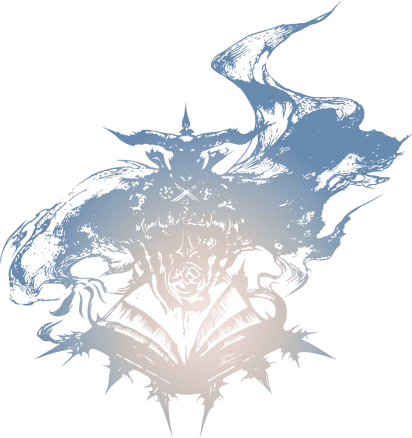
\includegraphics[width=0.9\columnwidth]{./art/images/ffta.png}}}
	\BgThispage
	\begin{center} 
\includegraphics[width=0.9\columnwidth]{./art/images/title.png} \end{center}
	\begin{center}
	\large
	\vspace{6cm} \hyperlink{gameplay}{\bf Reglas} \dotfill 1 \\
	\hspace{1cm} \hyperlink{adv}{Aventura} \dotfill 2 \\
	\hspace{1cm} \hyperlink{combat}{Combate} \dotfill 3 \\ 
	\vspace{0.5cm} \hyperlink{char}{\bf Personajes} \dotfill 5 \\
	\hspace{1cm} \hyperlink{cs}{Hojas de personaje} \dotfill 6 \\ 
	\hspace{1cm} \hyperlink{talent}{Talentos} \dotfill 8 \\ 
	\hspace{1cm} \hyperlink{job}{Oficios} \dotfill 10 \\ 
	\hspace{1cm} \hyperlink{equip}{Equipo} \dotfill 23 \\ 
	\vspace{0.5cm} \hyperlink{gm}{\bf Director del Juego} \dotfill 27 \\
	\hspace{1cm} \hyperlink{optrules}{Reglas opcionales} \dotfill 29 \\ 
	\hspace{1cm} \hyperlink{world}{Crear una aventura} \dotfill 30 \\ 
	\hspace{1cm} \hyperlink{monster}{Monstruos} \dotfill 31 \\ 
	\hspace{1cm} \hyperlink{coc}{Primera aventura} \dotfill 39 \\ 
	\end{center}
	\vfill
	\begin{center} 
	\footnotesize
	\textbf{
		 {\large Traducción: Juan Zabalza, David Rodríguez} \vspace{0.5cm}\\		
 Créditos: \\
 Wally Zielinski, Chris Giannoukos, Joshua Davis, Bruno Carvalho, Juan Altamirano, TastyRedTomato, Netzacoatl, Eldi13, Red7394, TaintedBalance, GM\_3826, The\_Fencer0, OmegaWeapon, Kaiten619, StorytellerZeke y todos los usuarios de nuestro \href{https://old.reddit.com/r/omegafantasy}{Subreddit} y nuestro \href{https://discordapp.com/invite/F5fpxMs}{Discord} \vspace{0.3cm} \\
 Final Fantasy, sus temas, arte y otros contenidos afiliados son propiedad de Square Enix Co., Ltd. Omega Fantasy es un proyecto de fans bajo la licencia \href{https://creativecommons.org/licenses/by-nc-sa/4.0/}{Creative Commons License (CC BY-NC-SA 4.0)} 2018. El proyecto se someterá a cualquier exigencia del propietario de la propiedad intelectual, Square Enix Co., Ltd. Como es un proyecto hecho por fans, nunca realizará cobros ni relaciones comerciales.
	}
	\end{center} 
\end{titlepage}

\hypersetup{linkcolor={blue!50!black},citecolor={blue!80!black},urlcolor={blue!80!black}}
\standardgeometry

\ofsection{Gameplay}
%
\ofquote{"You want quiet, you better take the next train."\\}{Lightning}
%
\begin{center} \includegraphics[width=\columnwidth]{./art/images/ff12.jpg} \end{center}
%
\accf{Final Fantasy} is a series of video games where each title features its unique story, world and characters.
Still they are part of the same series, not only due to recurring elements, but also because the stories focus on a group of heroes who face a great conflict.
\accf{Omega Fantasy} is a tabletop game that helps you to create Final Fantasy adventures with your friends and this release, named Omega~Fantasy~II, is an improved version of the original release.
To play, you only need dice, paper, pens, this book and at least one friend, but a group size of 4 to 6 is recommended.
To complete an adventure, your group needs to meet one or more times and play the game, each such gathering is called a \accf{Session}.
You do not necessarily have to meet in person, the game can also be played through online teleconferencing.
%
\ofpar
%
Choose one person to become the \accf{Game Master}~(shortened~\accf{GM}), who creates the game world and narrates the adventure by using the content and guidelines in this book.
During the game, he describes the environment to the players and how it reacts to their actions. 
The GM also takes the role of all non-player characters to narrate conversations and combat. 
Everyone else is a \accf{Player}, who creates and plays the game from the perspective of a \accf{Character} in the game world.
Player characters are the protagonists of the story who travel together as a \accf{Party} to explore the world, interact with people and fight against enemies. 
This book divided into three major sections: this first section explains the core rules and gameplay elements.
The second section details rules for creating and developing characters.
The final section focuses on the GM and offers a wide variety of guidelines and content for creating a game world. 
%
\vfill
%
\ofboxwithtitle{Example: Roleplaying\vspace*{0.15cm}}
{
	\newcommand{\nl}{\vspace{0.2cm}\\}
	\acc{Hironobu (Game Master):} You enter the Thunder Plains, which is a vast wasteland covered by thick fog and dark clouds.
	The locals have erected towers, that act as lightning rods, but you can see that lighting bolts often strike the ground in the open field.\nl
	\acc{Yoshinori (playing as Wakka):} We head north, not too near and not too far from the towers, ya?\nl
	\acc{Nobuo (playing as Rikku):} I wanna go home! I hate lightning! I hate thunder!\nl
	\acc{Tetsuya (playing as Auron):} This storm never stops. Better to cross quickly.\nl
	\acc{Hironobu (Game Master):} You can also see a small building nearby, that looks like an inn.\nl
	\acc{Nobuo (playing as Rikku):} Let’s go rest over there! Please? I'm too young to die!\nl
	\acc{Tetsuya (playing as Auron):} Fine, we rest. She is worse than the storm.
}
%
\vfill
%
Dice rolls are used to help decide the outcome of uncertain actions, but their exact nature depends on the context. 
This game only uses six-sided dice and we use \accf{d} shorthand to refer to such a die.
Furthermore, we use for example 4d to describe a roll of 4 dice, where the result is the sum of all rolled dice.
\accf{Checks} are the main tool to help the GM to decide and narrate the outcome of actions.
He can either ask players for checks or perform them himself in secret.
Checks are usually \accf{2d} rolls and higher numbers mean a better outcome for the roller. 
The minimum result to succeed is called Difficulty~(shortened \accf{DC}) and often has to be decided by the GM.
This DC should be based on the difficulty of the action and the proficiency of the actor.
Most DCs vary between 5 and 9, ones below this range are considered easy, while ones above it are very challenging.
%
\ofpar
%
Since checks are 2d rolls, the lowest and highest possible results are 2 and 12 respectively, which can be treated as unexpectedly good or bad, but still plausible outcomes.
A check can also have \accf{Advantage} or \accf{Disadvantage} when the circumstances have a substantial effect on the attempted action. 
In both cases, the check is made with 3d and with Advantage only the two highest and with Disadvantage only the two lowest dice are counted. 
Advantage and Disadvantage cancel each other out and do not stack.
%
%\ofpar
\clearpage
%
\ofboxwithtitle{Example: Advantage \& Disadvantage}
{
	Cloud meets Don Corneo in his mansion wearing a dress and make-up to convince him that he is a woman.
	The GM decides that this is a very difficult task (DC 10), because Cloud did not put much effort into his disguise. 
	But as the room is not well lit and the Don had a bit too much to drink, he also decides that the check has Advantage. 
	Cloud rolls 3d with the result [6,2,6] and since only the two highest dice count, he rolled the best possible outcome! 
	The GM decides that Don Corneo is not only convinced that Cloud is a woman, but he finds him so irresistible that he drags Cloud into his room for some time alone.
}
%
\ofpar
%
Another way to modify checks is through the use of \accf{Fortune Dice}.
At the start of each session, every player and the GM roll 1d and all results are written down and become the pool of Fortune Dice for this session.
During the session, after a player makes a roll, he or she can decide to remove one Fortune Die from the pool and use it to replace one die in the result of the roll.
However, the GM is also allowed to use Fortune Dice to modify the result of player rolls in the same manner.
This allows players to benefit from occasional strokes of luck or motivation while the GM can create moments of misfortune or complications.
In both cases, the person using the Fortune Die should try to give a narrative description of its effect.
Fortune Dice that are not used, are discarded at the end of each session.
%
\ofpar
%
\ofboxwithtitle{Example: Fortune Dice}
{
	Luneth explores the ancient Altar Cave. 
	As he walks towards a hole in the ground, the GM asks him for a DC~5 check to decide whether he can notice and avoid it.
	Luneth rolls [3, 4], which would pass the check.
	However, the GM decides to use a Fortune Die on his roll, the current pool of Fortune Dice includes \mbox{[1, 3, 3, 5]}.
	He removes the 1 from the pool and puts it in place of the 4 in Luneth's roll.  
	Accordingly, the roll is changed to [3, 1], which fails the check, and the remaining dice pool contains \mbox{[3, 3, 5]}.
	The GM describes this effect as follows: as he tries to carefully step around the hole, Luneth steps on a slippery rock, trips and falls into the hole.
	As a consequence, he finds himself an unknown and dangerous section of the cave and has find his way back to the exit.
}
%
\ofpar
%
\ofquote{"Why not? Nothing to lose but my life and I got that for free!"}{Setzer}\\\\
%
The party can explore the environment described by the GM at will.
They can look for specific things or wander around, but an appropriate amount of time passes while doing so.
The GM may draw a map of the party's current location as a visual aid. 
He is also free to impose checks on all exploration related actions, such as picking locks or detecting traps.
The party may go to sleep once per day to fully recover their HP and MP, even if unconscious.
To gain this benefit, they have to sleep in a comfortable place like an Inn or a Tent for multiple hours.
Throughout the adventure, the party will interact with other characters.
These non-player characters are voiced by the GM and accordingly the players talk from the perspective of their own characters.
To avoid confusion, it is important to clarify whether something you say is from the perspective of your character or from yours as player or GM.
During conversations, the GM may ask for checks, for example to decide whether an attempt to convince a character is successful.
%
\vfill
%
\ofquote{"You know what they say about the leading man, don't you? He never dies."}{Balthier}\\\\
%
Characters become stronger by gaining experience and we express the amount of experience a character has with \accf{Levels}.
Inexperienced adventurers start at Level 1 and can progress up to a maximum of Level 10 where they become renowned heroes. 
The GM decides when characters Level up, which we recommend for reaching adventure milestones.
Examples of milestones are important character development events, victories against powerful foes, or resolution of major conflicts. 
When going on dangerous adventures, \accf{Death} is always a real possibility, especially as a consequence of unwise decisions by the party. 
The adventure is officially over if all party members fall unconscious in battle, as this is usually followed by certain death. 
Characters may also die or leave the party under special circumstances in which case the GM takes control of him or her.
%
\ofpar
%
\ofboxwithtitle{Example: Experience \& Death}
{
	Kain betrays the party and joins their enemies. 
	He fights and defeats the rest of the party in combat, but chooses to let them stay alive.
	The GM takes control of Kain from now on, who leaves the party and becomes an antagonist.
	The party resolves to stop Kain's plan and his former player decides to create a new character that joins the party. 
	The GM rewards the party with a Level up for reaching a turning point in the adventure.
}
%
\vfill
%
Most adventures cover multiple sessions and sometimes a player might not be able to attend one.
In this case, the GM and the player can agree that his or her character leaves the party for the duration of that session to go on a \accf{Dispatch Mission}.
At the start of the next session, the character rejoins the party and the player explains what his or her character has tried to do during the previous session.
Then, the GM declares a DC for the Dispatch Mission and the player performs 3 checks with this DC.
If at least 2 out of the 3 checks succeed, then the mission was a success and if not, the character has failed in completing the mission.
%
\clearpage
\subsection*{\hypertarget{adv}{Adventuring}}
\addcontentsline{toc}{subsection}{Adventuring}
"Why not? Nothing to lose but my life... and I got that for free!"
\indent -- Setzer

\begin{center}
\includegraphics[width=\columnwidth]{./art/images/ff11.png} 
\end{center}

\vspace{0.1cm}

\subsubsection*{\hypertarget{check}{Checks}}
Checks are the main tool to help the GM to decide and narrate the outcome of actions.
He can either ask players for checks or perform them himself in secret.
Checks are usually \textbf{2d} rolls and higher numbers mean a better outcome for the roller. 
The minimum result required to succeed is called Difficulty~(shortened \textbf{DC}) and often has to be decided by the GM.
He should base this DC on the difficulty of the action and the proficiency of the actor in it.
Since checks are 2d rolls, the lowest and highest possible results are 2 and 12 respectively, which can be treated as unexpectedly good or bad, but plausible outcomes.
A check can also have \textbf{Advantage} or \textbf{Disadvantage} when the environment substantially affects the attempted action. 
In both cases the check is made with 3d and with Advantage only the two highest and with Disadvantage only the two lowest dice are counted. 
The table below shows rough categories for DCs.

\vfill

\begin{tcolorbox}[colback=white, tabularx={@{\hspace{1cm}} p{0.5\columnwidth} p{0.3\columnwidth}},sharp corners=south,colframe=accent, 
	title=\begin{center}\textbf{Difficulty Categories}\end{center}]	
	\textbf{Action} 	& \textbf{DC} \\
	\hline 	Very Hard 	& 11 - 12 \\
	\hline	Hard 		& 8 - 10 \\
	\hline  Medium 		& 5 - 7 \\
	\hline  Easy 		& 1 - 4 \\
\end{tcolorbox}

\vfill

\example{Checks}
{
Cloud meets Don Corneo in his mansion wearing a dress and make-up to convince him that he is a woman.
The GM decides that this is a very difficult task (DC 11), because Cloud did not put much effort into his disguise. 
But as the room is not well lit and the Don had a bit too much to drink, he also decides that the check has Advantage. 
Cloud rolls 3d with the result [6,2,6] and since only the two highest dice count, he rolled the best possible outcome! 
The GM decides that Don Corneo is not only convinced that Cloud is a woman, but he finds him so irresistible that he drags Cloud into his room for some time alone.
}

\pagebreak

\subsubsection*{Exploration}
The party can explore the environment described by the GM at will.
They can look for specific objects or wander around, but an appropriate amount of time passes while doing so.
The GM may draw a map of the party's current location as a visual aid. 
He is also free to impose checks on all exploration related actions, such as picking locks or detecting traps.
The party may go to sleep once per day to fully recover their HP and MP, even if unconscious.
To gain this benefit, they have to sleep in a comfortable place like an Inn or a \hyperlink{item}{Tent} for multiple hours.

\vfill

\subsubsection*{Social Interaction}
Throughout the adventure, the party will interact with other characters.
These non-player characters are voiced by the GM and accordingly the players talk from the perspective of their own characters.
To avoid confusion, it is important to clarify whether something you say is from the perspective of your character or from yours as player or GM.
During conversations, the GM may ask for checks, for example to decide whether attempt to convince a character is successful.

\vfill

\subsubsection*{Experience}
Characters become stronger by gaining experience and we express the amount of experience a character has with \textbf{Levels}.
Inexperienced adventurers start at Level 1 and can progress up to a maximum of Level 10 where they become renowned heroes. 
The GM decides when characters Level up, which we recommend for reaching adventure \mbox{\textbf{\hypertarget{ms}{Milestones}}}.
Such Milestones are for example important character development events, victories against powerful foes, or resolution of major conflicts. 

\vfill

\subsubsection*{Death}
When going on dangerous adventures, death is always a real possibility, especially as a consequence of unwise decisions by the party. 
The adventure is officially over if all party members fall \textbf{unconscious} in battle, as this is usually followed by certain death. 
Characters may also die or leave the party under special circumstances in which case that character becomes unplayable for their player. 

\vspace*{0.7cm}

\example{Experience \& Death}
{
	Kain betrays the party and joins their enemies. 
	He duels his friend Cecil and defeats him and the rest of the party in combat, but chooses to let them stay alive.
	The GM takes control of Kain from now on, who leaves the party and becomes an antagonist.
	The party resolves to stop Kain's plan and his former player decides to create a new character that joins the party. 
	The GM rewards the party with a Level up for reaching a turning point in the adventure.
}

\pagebreak

\ofsubsection{Combat}
%
\ofquote{"Enough expository banter. It's time we fight like men. And ladies. And ladies who dress like men."\\}{Gilgamesh}\\
%
\includegraphics[width=\columnwidth]{./art/images/ff13-2.jpg}
%
\vfill
%
\accf{Combat} encounters are played out in a series of rounds (shortened~\accf{r}) and during a round, every combatant takes one turn.
At the start of the battle, both parties choose who takes the first turn in each round on their side and the GM the decides which side goes first.
Then, the opposing parties take alternating turns until every combatant has taken one and the round is finished.
The turn order for each side is decided as follows: at the end of their turns, every combatant chooses an ally who has not taken a turn in this round and should take the next one for their side.
If one side has more combatants, they can take consecutive turns at the end of the round until every participant has taken one.
Announce the start and end of each round to avoid confusion.
When a party ambushes the other before combat, the GM can decide that they gain a \accf{surprise round}.
In this case, only the surprising party acts in the first round before the battle continues as usual.
%
\vfill
%
Combat proficiencies are determined by the following 7 numerical \accf{attributes}.
Whenever a calculation results in a non-integer value, the result is always rounded down.
%
\ofgap
%
\ofmbox{\oficonhp\accf{Hit Points (HP)}} increase your durability. You have a maximum and a current number of HP, if your current HP falls to 0 you fall unconscious. \ofrow
\ofmbox{\oficonmp\accf{Mana Points (MP)}} are the resource required for using abilities such as Magic and Techs. Similar to HP, you have a maximum and a current number of MP. \ofrow
\ofmbox{\oficonstr\accf{Strength (STR)}} increases the damage dealt by your physical attacks. \ofrow
\ofmbox{\oficondef\accf{Defense (DEF)}} increases your resilience against physical damage. \ofrow
\ofmbox{\oficonmag\accf{Magic (MAG)}} increases the potency of your healing and attacking spells. \ofrow
\ofmbox{\oficonres\accf{Resistance (RES)}} increases your resilience against magical damage. \ofrow
\ofmbox{\oficonagi\accf{Agility (AGI)}} allows you to evade physical attacks and determines how quickly you can move.
%
\newpage
%
During your turn you can, in any order, move a distance of your AGI+1 units and take an action.
Below is a list of \accf{combat actions}, but the GM may allow any other action that can be completed in a similar amount of time:\ofgap
%
\ofmbox{\oficonattack\accf{Attack:}}
You attack an enemy with your weapon. 
He may evade by passing an \accf{evasion check} with a DC of 12 minus his AGI. 
If he fails the check, you reduce the target's HP by your weapon's DMG plus your STR.
If the evader rolls a 2, you make a \accf{critical hit}, doubling your usual damage. 
If he rolls a 12, not only does your Attack miss, but the evader makes an Attack action on you instead, which you cannot evade.\ofgap
%
\ofmbox{\oficonmagic\accf{Magic:}}
You cast a spell by spending MP, choosing a target within its range and concentrating for a duration.
While concentrating, you cannot take actions or evade. 
After the cast time is up, the spell's effect occurs on the target right \accf{before your turn} and cannot be evaded even if you are not in range anymore.
If the spell deals damage or restores HP, add your MAG to the amount.
Every spell's description has information on its cast time, MP cost, target, range and effect.\ofgap
%
\ofmbox{\oficontech\accf{Tech:}}
You use a non-magical ability. 
Techs are used the same way as magic, but their damage and healing is amplified by your STR instead of your MAG, 
except if their use already includes this bonus in another way, for example by involving an Attack.\ofgap
%
\ofmbox{\oficondefend\accf{Defend:}} All total damage that you receive by Attacks until your next turn is halved. \ofgap
%
\ofmbox{\oficonitem\accf{Item:}} You use an Item from your inventory on yourself or someone within 1u.\ofgap
%
\ofmbox{\oficonreequip\accf{Re-Equip:}} Swap a Materia or Equipment piece that you are wearing against one from your Inventory.\ofgap
%
\ofmbox{\oficondash\accf{Dash:}} Move to a location up to AGI +1 units away.\\\\
%
Apart from Magic and Techs, characters can also learn the following \accf{special abilities}: \ofrow
\ofmbox{\oficonpassive\accf{Passive:}} Effects that are permanently active. \ofgap
\ofmbox{\oficonreaction\accf{Reaction:}} Allow you to take certain actions on someone else's turn under specific conditions.
%
\vfill
%
\ofboxwithtitle{Example: Combat}
{
	Squall (4 DEF, 3 AGI, 1 RES) and Seifer (6 STR, 2 MAG) decide to duel.
	Both are wielding a gunblade~(1d DMG) and the GM decides that Seifer takes the first turn.
	He begins casting Firaga (6d DMG, 1r Time) by spending 12~MP, choosing Squall as its target and concentrating.
	Squall uses his turn to Defend.
	It's Seifer's turn again, so Firaga takes effect and Squall suffers \mbox{6d+2-1} damage. 
	Seifer can still take his turn, so he also Attacks. 
	Squall makes a \mbox{DC 12-3} evasion check, but by rolling [1, 1] he fails and suffers a Critical Hit! 
	Seifer hits him right above the nose with his blade, inflicting \mbox{1d+6-4} damage (Defend and Critical Hit cancel each other out) and leaving a scar.
}
%
\clearpage
%
\newcommand{\elemicon}[1]{\hspace*{-0.14cm}#1\hspace*{-0.14cm}}
All damage dealt has one of two basic types.
Unless specified otherwise, Attacks and Techs are of \accf{physical} type, while Magic and Items are of \accf{magical} type.
When you receive physical damage, subtract your DEF from the amount and when you receive magical damage, subtract your RES from the amount.
In addition, damage can have an elemental type to which combatants can have \accf{Weaknesses} or \accf{Resiliences}. 
When resilient, you only suffer half the usual damage and when weak, you suffer double the usual damage. 
Resilience and Weakness cancel each other out and do not stack.
The following elemental types exist: \elemicon{\fire}ire, \elemicon{\ice}ce, \elemicon{\lightning}ightning, W\elemicon{\water}ter, \elemicon{\earth}arth, \elemicon{\wind}ind, \elemicon{\holy}oly and \elemicon{\dark}ark.
%
\vfill
%
\accf{Units} (shortened \accf{u}) are the basis to measure distance, where 1u is roughly 1m or 3ft.
Characters usually occupy a circle of 1u in diameter in top view. 
Effect distances are described by their Range and Target.
\accf{Range} is the maximum distance between the center of the caster and the center of the effect. 
An effect with range Self is centered at the caster, and one with range Weapon has the same range as the used weapon.
\accf{Target} is the area of the effect as a maximum distance from its center. Unless stated otherwise, everyone fully or partially in the target area is affected, including allies.
An effect with target Single affects only a single entity.
The following illustration shows the use of a ranged effect in the normal case and with the two special target shapes Line and Front. 
%
\begin{figure}[h!]
		\begin{tikzpicture}[]
		\tikzstyle{test}=[thick, draw, circle, align=center]					
		%Normal
		\node[fill=blue!30!white, test,minimum size = 0.75cm](caster)at (0,0) {};
		\node[](t2)at (0,-0.6) {\bf\footnotesize Normal};
		\node[fill=red!10!white, test, very thick, dashed ,minimum size = 2.8cm](tarea)at (0,2) {};
		\node[fill=red!60!white, test,minimum size = 0.75cm](target)at (0,2) {};
		\node[fill=red!60!white, test,minimum size = 0.75cm](target)at (-1.2,1.2) {};
		\draw[thick, ->](0,0) -- node[] {}(0,2);
		\draw[thick, ->](0,2) -- node[] {}(-1.4, 2);
		\node[rotate=90](t1)at (0.2,1.12) {\bf\footnotesize Range};
		\node[](t2)at (-0.85,2.15) {\bf\footnotesize Target};
		\node[](t3)at (0,2) {\bf\footnotesize x};
		\node[](fi)at (-0.375,2.6) {\bf\footnotesize |};
		\node[](se)at (0.375,2.6) {\bf\footnotesize |};
		\draw[thick, -](0.375,2.6) -- node[] {}(-0.375,2.6);
		\node[](sca)at (0,2.8) {\bf\footnotesize 1u};		
		%Line
		\node[draw, fill=red!10!white, rectangle, very thick, dashed ,minimum height = 3.5cm, minimum width=0.75cm](tarea)at (2.6,1.6) {};
		\node[fill=blue!30!white, test,minimum size = 0.75cm](caster)at (2.6,0) {};
		\node[](t2)at (2.6,-0.6) {\bf\footnotesize Line};
		\node[fill=red!60!white, test,minimum size = 0.75cm](target)at (3.1,2.8) {};
		\draw[thick, ->](2.6,0) -- node[] {}(2.6,3.3);
		\node[rotate=90](t1)at (2.8,1.3) {\bf\footnotesize Target};
		\node[](t3)at (2.6,0) {\bf\footnotesize x};		
		%Front
		\draw[fill=red!10!white, test, very thick, dashed] (4,0) arc (180:0:1.6cm);
		\draw[dashed, very thick, -](4,0) -- node[] {}(7.2,0);
		\node[fill=blue!30!white, test,minimum size = 0.75cm](caster)at (5.6,0) {};
		\node[](t2)at (5.6,-0.6) {\bf\footnotesize Front};
		\draw[thick, ->](5.6,0) -- node[] {}(5.6,1.6);
		\node[rotate=90](t1)at (5.8,1) {\bf\footnotesize Target};
		\node[fill=red!60!white, test,minimum size = 0.75cm](target)at (4.8,1) {};
		\node[fill=red!60!white, test,minimum size = 0.75cm](target)at (6.8,0.9) {};
		\node[](t3)at (5.6,0) {\bf\footnotesize x};
		\end{tikzpicture}
\end{figure}
%
\vfill
%
\accf{Fields} are effects that occupy an area on the battlefield and cause harm to anyone inside.
They can be caused by abilities or natural causes such as steam or fog.
If at any point in your turn, you come into contact with a Field, you suffer its effect until the end of your turn.
Fields do not stack, when a new Field is created in the same area as an existing one, the previous Field is destroyed.
All Field effects are listed below.
%
\\\\
%
\oftable{p{0.17\columnwidth} p{0.77\columnwidth}}
{\accf{Field} & \accf{Effect}}
{
	Slow & You can only move half your usual distance.\ofrow
	Hot  & You receive fire damage equal to 10\% of your maximum HP.\ofrow
	Slippery & Make a DC~8 check and suffer Immobile upon failure.\ofrow
	Obscure & You suffer Blind.
}
%
\newpage
%
\accf{Status Effects} alter your the combat potency for a limited duration.
Combatants can suffer multiple different Status Effects at once, but applying the same one twice only refreshes its duration. 
They can also be \accf{Immune} to certain Status Effects, in which case they are not affected by them.
Also, if a combatant suffers two opposite Status Effects, for example Poison and Regen, they negate each other and are both removed.
Below is a list of all Status Effects. 
%
\vfill
%
\ofmbox{\oficonko\accrf{KO:}}
You are unconscious and your turns are skipped.
You suffer KO when your current HP drops to 0 and your HP cannot be increased until this status is removed.  
Immunity against KO only makes you immune against effects that cause it when above 0 HP.\ofgap
%
\ofmbox{\oficonblind\accrf{Blind:}} Whenever you Attack an enemy, he has Advantage on the evasion check. \ofgap
%
\ofmbox{\oficondestr\hspace*{-0.1cm}\oficondedef\hspace*{-0.1cm}\oficondemag\hspace*{-0.1cm}\oficonderes\accrf{DeATR:}} The according attribute is reduced by 1 plus half your current Level to a minimum 0. For example, DeSTR reduces your STR by 4 when you are Level 7.  \ofgap
%
\ofmbox{\oficonimmobile\accrf{Immobile:}} You are unable to move.\ofgap
%
\ofmbox{\oficonpoison\accrf{Poison:}} You take damage equal to 10\% of your maximum HP at the start of each of your turns, but cannot fall below 1 HP due to this effect.\ofgap
%
\ofmbox{\oficonsilence\accrf{Silence:}} You cannot begin casting Magic or using Techs, but you can still Attack.\ofgap
%
\ofmbox{\oficonslow\accrf{Slow:}} During your turn, you can either move or take an action but not both.\ofgap
%
\ofmbox{\oficonsleep\accrf{Sleep:}} You cannot move or take any action. This status is removed when you take any damage.\ofgap
%
\ofmbox{\oficonzombie\accrf{Zombie:}} All healing effects are reversed for you. Healing reduces your HP and effects that normally remove KO, inflict it to you instead.\ofgap
%	
\ofmbox{\oficonblink\accgf{Blink:}} Whenever you are targeted by an Attack, you have Advantage on the evasion check. \ofgap
%
\ofmbox{\oficonenstr\hspace*{-0.1cm}\oficonendef\hspace*{-0.1cm}\oficonenmag\hspace*{-0.1cm}\oficonenres\accgf{EnATR}} The according attribute is increased by by 1 plus half your current Level. For example, EnMAG increases your MAG by 2 when you are Level 3. \ofgap
%
\ofmbox{\oficonhaste\accgf{Haste:}} During your turn, you can either make an additional action or movement. \ofgap
%
\ofmbox{\oficonregen\accgf{Regen:}} You regain HP equal to 10\% of your maximum HP at the start of each of your turns.
%
\vfill
%
\ofboxwithtitle{Example: Status Effects}
{
	Noctis and Prompto fight Malboro. 
	The monster uses its Bad Breath ability to inflict multiple Status Effects.
	Prompto suffers Sleep and Poison.
	At the start of his turn he loses 3 HP (his maximum HP is 37) and he cannot move or take actions.
	Noctis suffers Silence and Blind.
	He cannot use abilities, so he tries to Attack Malboro. 
	The monster~(2~AGI) rolls [1,6,4] on the evasion check, barely passing the DC 12-2 check due to Advantage.
}
%
\clearpage

\ofsection{Jogadores}
%
\ofquote{"Eu sou O Basch fon Rosenburg!"\\}{Vaan}\\\\
%
\includegraphics[width=\columnwidth]{./art/images/ff10-2.jpg}
%
\vfill
%
Cada jogador cria um \accf{Personagem} que é um protagonista no mundo de jogo criado pelo MJ. 
Para criar um personagem de Nível 1, copie ou imprima a \accf{Ficha de Personagem} da próxima página. 
Ela permite a você acompanhar vários aspectos de seu personagem, há também um exemplo de ficha preenchida, como guia. 
Escolha o \accf{Nome} de seu personagem e faça uma descrição curta sobre ele. 
Resuma a \accf{História} dele e explique suas motivações para se juntar ao grupo, considerando que o mais provável é que essa seja a sua primeira aventura séria. 
Escolha então uma \accf{Profissão} como explicado abaixo. 
Por fim, a subseção de \accf{Equipamento} explica como você pode personalizar os equipamentos iniciais de seu personagem. 
A tabela à direita resume os benefícios fornecidos em Níveis subsequentes, todos explicados em detalhes dentro desta seção.
%
\vfill
%
A \accf{Profissão} de seu personagem determina a proficiência em combate dele, incluindo habilidades, atributos e especialidade com equipamentos. 
Todas as profissões são detalhadas nas suas descrições logo após as fichas de personagem. 
Imprima ou copie a descrição daquela escolhida por você para usar como uma segunda página de sua ficha de personagem.
Os atributos de seu personagem iniciam em 0 e aumentam ao progredir em uma profissão. 
A descrição de cada uma delas mostra os atributos e habilidades recebidos em cada Nível, assim como todos os tipos de equipamentos que o seu personagem usa. 
Quando o seu personagem alcança o Nível 3, você tem que decidir entre um ou dois \accf{Arquétipos}. 
Arquétipos representam diferentes especializações de uma profissão e fornecem habilidades e atributos adicionais.
%
\newpage
%
\ofboxwithtitle{Exemplo: Criação de Personagem}
{
	Nós criamos um personagem chamado Vaan, que tem 17 anos, um garoto humano, loiro e de aparência atlética. 
	Vaan é um órfão que se vira na cidade grande roubando e geralmente age como uma figura paterna para os outros órfãos. 
	Ele sonha em ter sua própria aeronave e um dia ser um pirata dos céus. 
	Nós escolhemos a profissão Ladrão e de sua tabela de atributos, nós determinamos o PV máximo~(20), PM máximo~(19) e AGI (4), todos os outros atributos começam em 0. 
	Nós também anotamos que ele aprende a técnica Roubar. 
	Por fim, de nossos 1500G iniciais, compramos uma faca de Mithril, um Colete de Mithril, uma Pena de Fênix e 2 poções, o que nos deixa com 300G sobrando.
}
%
\vfill
%
\oftable{p{0.25\columnwidth} p{0.7\columnwidth}}
{\accf{Nível} & \accf{Benefício ganho}}
{
	1 & Profissão, Equipamento iniciante \ofrow
	2 & Talento \ofrow
	3 & Arquétipo \ofrow
	4 & Quebra de Limite, Equipamento avançado\ofrow
	5 & Esper \ofrow
	6 & Especialização \ofrow
	7 & Especialização \ofrow
	8 & Especialização, Equipamento Especialista \ofrow
	9 & Especialização \ofrow
	10 & Especialização
}
%
\vfill
%
Nos Níveis marcados como \accf{Especialização}, escolha um dos seguintes benefícios para seu personagem.\ofrow
\ofbullet{No início de cada uma das sessões, adicione um 6 extra à reserva de Dados de Fortuna.}
\ofbullet{Ganhe uma segunda escolha de Esper.}
\ofbullet{Ganhe uma segunda escolha de Talento.}
\ofbullet{Ganhe um segundo Modo Limite, permite a você obter Pontos Limite de 2 fontes. Além disso, o alcance máximo de sua Quebra de Limite é aumentado em 2.}
\ofbullet{Ganhe acesso ao segundo Arquétipo de sua profissão. Você pode alternar entre os dois sempre que for dormir e seus atributos e habilidades mudam de acordo com aquele ativo no momento.}
\ofbullet{Ao usar Magia, Técnica ou habilidade de Reação de seu Arquétipo, o custo de seu PM é reduzido pela metade e você ganha 1 Ponto Limite.}
\ofbullet{Armas e armaduras ganham um espaço de Matéria adicional enquanto estiverem equipadas.}
\ofbullet{Ganhe a capacidade de equipar uma arma ou armadura adicional à sua escolha.}
\ofbullet{Escolha um bônus da lista a seguir. Não é possível escolher o mesmo benefício mais de uma vez: PV+5, PM+5, FOR+1, DEF+1, MAG+1, RES+1.}
%
\clearpage
%
\ofcs{}
%
\ofcs{
	name=Lightning,
	%
	description={%
		\vspace*{-0.5cm}
		\begin{multicols}{2}
			Idade: 21\\Raça: humano\\Cabelo: rosa\\Altura: 1.70m\\Destra\\ Determinada\\ Fria
			\columnbreak\vspace*{-1.7cm}\\
			\hspace*{-1cm}\includegraphics[width=1\columnwidth]{./art/charactersheets/claire.jpg}
		\end{multicols}
		\vspace*{-0.9cm}
	},
	%
	story={\\
		Meus pais morreram quando eu era jovem.
		Eu criei minha irmã, Serah, e me alistei no exército, no qual me tornei sargento.
		Mas agora Serah está em perigo, então eu tenho que deixar o exército e para encontrá-la. \\\\\\
		"Não é uma questão de ser capaz ou não.\\Há coisas na vida que você simplesmente faz."
	},
	% 
	hpcur=19, hpmax=91, mpcur=13, mpmax=85, agi=3, movement=4u, evasiondc=9, str=5, def=3, mag=7, res=2, 
	%
	level=8, job=Mago Vermelho, archetype=Devastador\phantom{1234567}, talent=Corporações Guardião,
	%
	abilities={Cura, Fogo, Nevasca, Raio, Cegueira,\\ Veneno, Esuna, AnuElemento},
	specials={Sobrepujar, Conjuração Rápida}, status={Cegueira (1r), AnDEF (2r)},
	%
	limitbreak=Raiara, limitmode=Bravura, limitpoints=\ofcslimitbarfilled, 
	limitdesc={Uma chuva de raios irrompe dos céus sobre um inimigo dentro de 5u e todos a 2u dele. Todos os alvos afetados sofrem 2d+8 de dano de raio.},
	%
	summon=Odin, summonused=yes, summonsupport={Realize um pequeno ritual para invocar o cavalo de Odin, Sleipnir.\\}, summonability={Um alvo no campo de batalha é afetado por KO se falhar num teste de DF~8 ou recebe dano igual a 3x seu nível se passar.},
	%
	weapon=Lâmina Pistola Dobrável, weaponbox=\ofcsweaponboxexpert, weaponeffect=Ataque à distância após a habilidade, weapontype= contra-ataque de 11 a 12 no teste de evasão, armor=Uniforme da Corporação Guardiã, armorbox=\ofcsarmorboxbeginner, armortype=DEF~+1, accessory1=Bracelete do Poder, accessory1effect=FOR~+1,
	%
	gil=2009, inventory={\\Faca de sobrevivência, 5x Granada, 5x Poção maior,\newline3x Remédio, 2x Pena da Fênix, 1x Elixir}
}
%
\clearpage
\ofcs{}
\ofcs{
	name=Lightning,
	%
	description={%
		\vspace*{-0.5cm}
		\begin{multicols}{2}
			Age: 21\\Race: human\\Hair: rose\\Height: 1.70m\\Right-Handed\\ Determined\\ Cold
			\columnbreak\vspace*{-1.7cm}\\
			\hspace*{-1cm}\includegraphics[width=1\columnwidth]{./art/charactersheets/claire.jpg}
		\end{multicols}
		\vspace*{-0.9cm}
	},
	%
	story={\\
		Both of my parents died when I was young. 
		I raised my sister Serah and joined the army where I became a sergeant. 
		But now Serah is in danger so I have quit the army to find her. \\\\\\
		"It's not a question of can or can't. There are some things in life you just do."
	},
	% 
	hpcur=17, hpmax=99, mpcur=13, mpmax=71, agi=3, movement=4u, evasiondc=9, str=6, def=3, mag=5, res=3, 
	%
	level=8, job=Red Mage, archetype=Ravager\phantom{1234567}, talent=Guardian Corps,
	%
	abilities={Cure, Fire, Blizzard, Thunder, Blind,\\ Poison, Esuna, NulElement},
	specials={Overwhelm, Swiftcast}, status={Blind (1r), EnDEF (2r)},
	%
	limitbreak=Thundara, limitmode=Brave, limitpoints=\ofcslimitbarfilled, 
	limitdesc={A barrage of lightning strikes descends upon an enemy within 5u and everyone within 2u of him. All affect targets suffer 2d+8 lightning damage.},
	%
	summon=Odin, summonused=yes, summonsupport={Conjure horse Sleipnir}, summonability={Target on the battlefield suffers KO with DC~8 check or 3 times Level damage otherwise.},
	%
	weapon=Foldable Gunblade, weaponbox=\ofcsweaponboxexpert, weaponeffect=Ranged attack after ability, weapontype=crit on 11 or 12 enemy evasion check, armor=Guardian Corps Uniform, armorbox=\ofcsarmorboxexpert, armortype=DEF~+1, accessory1=Power Armlet, accessory1effect=STR~+1,
	%
	gil=2009, inventory={\\Survival Knife, 5x Bomb Fragment, 5x Hi-Potion\\ 3x Remedy, 2x Phoenix Down, 1x Elixir}
}
\ofsubsection{Talents}
%
\ofquote{"Sweet Christmas, it's a talking turtle!"\\}{Bartz}\\
%
\includegraphics[width=\columnwidth]{./art/images/ff3.jpg}
%
\vfill
%
\accf{Talents} are non-combat related skills that a character is especially proficient with.
Every character gains a Talent when they reach \accf{Level 2}, but the GM may allow them to gain additional Talents under special circumstances.
Below is a list of Talents, the GM may also allow players to create their own Talents using the ones given as examples.
%
\ofpar
%
\ofboxwithtitle{Example: Talents}
{
	Kefka leads the army of the Gestahlian empire in a siege on Doma Castle, who are accused of supporting rebel groups.
	Their first attempt at a frontal attack fails spectacularly.
	The castle is well fortified and led by a powerful soldier named Cyan.
	Kefka devises a vicious plan to secure victory: 
	he uses his Clown Talent to create a powerful liquid poison that leaves no trace.
	Despite protest among his allies, he pours the poison into Doma's water supply, resulting in the death of most its population.
	Although Cyan survives, Doma is severely weakened and the Gestahlian army is able to take the castle with ease.
}	
%	
\ofpar\vfill
%
\oftalent{Alchemist}
{
	After every successful battle against monsters you can create a Bomb Fragment, Arctic Wind or Lightning Gem out of their remains. 
}
\vfill
\oftalent{Apothecary}
{
	You can spend an hour to create a Potion or a Remedy from ingredients found in nature or stores.
}
\vfill
\oftalent{Archylte Hunter}
{
	You have Advantage on all checks related to hunting or fishing.
}
\vfill
\oftalent{Artist}
{
	Given enough time, you can create beautiful works of art in the form of paintings, sculptures or photographs.
	If you find interested buyers, each piece is worth an amount Gil up to 100 times your current Level.
}
\vfill
\oftalent{Blue Mage}
{
	You can quickly learn most simple non-combat skills by carefully observing someone proficient during the act for a while. 
	Such simple skills are for example cooking a meal or riding a Chocobo.
}
\newpage
\oftalent{Book Worm}
{
	You can understand the most important contents of any book or text in a matter of minutes.
}
\vfill
\oftalent{Calculator}
{
	Given enough time, you can solve any mathematical problem.
	Furthermore, you can make reliable numerical estimates, e.g. for various distances or the amount of people in a large group.
}
\vfill
\oftalent{Camping Again}
{
	While outside, you can spend an hour to build a comfortable shelter to spend the night out of materials found in nature.
}	
\vfill
\oftalent{Carpenter}
{
	Given enough time and materials, you can create and repair any object that is mostly made out of wood, such as furniture or vehicles.
}
\vfill
\oftalent{Chocobo Sage}
{
	You can comfortably tame and build friendships with friendly animals and monsters.
}
\vfill
\oftalent{Cid's Apprentice}
{
	Given enough time and materials you are able to repair any broken machine or vehicle. 
}
\vfill
\oftalent{Clown}
{
	You can spend multiple hours to create a potent poison out of materials found in nature or in stores.
	The poison is tasteless and odorless and can only be detected by experts such as yourself.
	A character that consumes the poison makes a DC~8 check and suffers KO upon failure.
}
\vfill
\oftalent{Concealer}
{
	You can spend a few minutes of time to change your appearance such that you are not easily recognized.
	People who have seen you before have to pass a DC~9 check to realize the deception.
}
\vfill
\oftalent{Conjurer}
{
	You can spend a few minutes to perform a ritual that creates an illusion of a character, monster or object.
	To understand that it is an illusion, a character either has to touch it or pass a DC~8 check.
}
\vfill
\oftalent{Dedicated Driver}
{
	You are able to perfectly drive or navigate any vehicle including ships and airships. 
}
\vfill
\oftalent{Deja Vu}
{
	When you meet a new character, you may declare that you have met them before.
	In this case, the GM determines your connection.	
	You can only use this effect a total of 3 times in the entire adventure.
}
\vfill
\oftalent{Flower Girl} 
{
	You can identify any plant and know how to grow them even in very unfavorable conditions.
}
\vfill
\oftalent{Force of Nature}
{
	You have Advantage on all checks that require proficiency and experience related to nature, such as following tracks in a forest. 
}
%
\newpage
%
\oftalent{Guardian Corps} 
{
	You do not suffer damage by falling from any height.
}
\vfill
\oftalent{Hope's Assistant} 
{
	Given any object or trace, you can determine its date and place of creation accurately.
}
\vfill
\oftalent{Investor}
{
	You can lend Gil at an interest to any business of your choice.
	After at least one week has passed, you can collect back your money plus an additional amount equal to 10\% of the loan.
}
\vfill
\oftalent{It's a Unix System}
{
	You have no problems with understanding and using even the most complex technologies such as computer or communication systems.
}
\vfill
\oftalent{King's Shield}
{
	You have Advantage on all checks that rely on pure strength such as lifting heavy objects or opening tight jar lids.
}
\vfill
\oftalent{Leading Man}
{
	You have Advantage on all checks that involve impressing or persuading through speech. 
}
\vfill
\oftalent{Let's Mosey}
{
	You can perfectly imitate the mannerisms of a person that you have spent a few days of time with.
}
\vfill
\oftalent{Llymlaen's Disciple}
{
	You never lose your way, even in locations that you are unfamiliar with.
	Moreover, you have no issues with reading maps or following given directions. 
}
\vfill
\oftalent{O'aka XXIV}
{
	When you sell used goods, you can convince the buyer to pay the original value.
}
\vfill
\oftalent{Opera Floozy}
{
	You have Advantage on all checks that involve acting, singing, dancing or performing.
}
\vfill
\oftalent{Orator}
{
	Whenever you talk to a character that you know, you can spend a few minutes of time to motivate and inspire them.
	The character then has Advantage on the next check that they perform.
}
\vfill
\oftalent{Pharmacologist}
{
	Whenever you use an Item outside of combat, the target additionally regains an amount of HP equal to your current Level. 
}
\vfill
\oftalent{Pyrotechnician} {
	You can spend an hour to create an explosive from materials found in stores or nature.
	An explosive takes a few minutes to set up and can for example be used as a distraction or to open a hole in a wall.
}
\vfill
\oftalent{Scan}
{
	While you are not in combat, you can observe a character or monster and immediately know their Level and current HP.
}
\vfill
\oftalent{Sceptic}
{
	You have Advantage on checks related to noticing whether someone is lying or withholding information.
}
%
\newpage
%
\oftalent{Shrouded One} 
{
	You have Advantage on all checks related to hiding or staying undetected.
}
\vfill
\oftalent{Simdemehkiym}
{
	You are fluent in 2 languages and can learn new ones in a matter of days.
}
\vfill
\oftalent{Skywatcher}
{
	You can accurately predict the weather in your current location for the next week.
}
\vfill
\oftalent{Spira's Historian}
{
	You have knowledge on most historical facts and you have Advantage on checks related to making connections to historical events. 	 
}
\vfill
\oftalent{Spoony Bard}
{
	You have perfectly mastered one music instrument of your choice and you can play any music piece on any music instrument to a convincing degree.
}
\vfill
\oftalent{Starplayer}
{
	You are among the best in the world in one sport or game of your choice.
}
\vfill
\oftalent{Strange Gourmand}
{
	You can spend an hour to prepare a tasty meal from almost anything that can be found in stores or in nature.
}
\vfill
\oftalent{Story Teller}
{
	You have Advantage on all checks related to telling convincing lies or omitting the truth.
}
\vfill
\oftalent{Tantalus Performer}
{
	You can use magic to create simple illusions, including various voices and noises, small flames and gusts of wind.
}
\vfill
\oftalent{Telepathy}
{
	You can send telepathic messages to any person that you can see within 10u.
}
\vfill
\oftalent{Theologian}
{
	You have perfect knowledge on all religions in the world, including their deities, customs and factions.
}
\vfill
\oftalent{Thief's Caution}
{
	You have Advantage on all checks related to noticing ambushes or hostile intentions of characters.
}
\vfill
\oftalent{Wandering Gambler}
{
	You have Advantage on all checks related to in-game random events such as card draws.
}
\vfill
\oftalent{Walkthrough}
{
	You have Advantage on all checks related to finding hidden locations and passages. 	 
}
\vfill
\oftalent{Weaver}
{
	Given enough time and materials, you are able to create any kind of cloth or clothing.
}
\vfill
\oftalent{Yin \& Yang}
{
	While not in combat, you can meditate for a few minutes to reduce your MP by an amount of your choice and increase your HP by the same amount.
}
%
\clearpage
\ofsubsection{Jobs}
%
%
%
%
%
\ofjob{Bard}
{
	\ofquote{"Welcome to your doom, starring me!"\\}{Rikku}\\\\
	\includegraphics[width=\columnwidth]{./art/jobs/bard.jpg}\ofrow
	\accf{Bards} blur the lines between art and war.
	They can perform songs and dances that bestow powerful benefits for allies and vicious handicaps for enemies.
	Even though Bards are not the most powerful duelists, they can often turn the tide of a battle in unexpected ways.
}
{Dagger}{Light Armor or Robe}{
	Level 1: & HP~+19 & MP~+20 & AGI~+3 & RES~+1  \\
	Level 2: & HP~+10  & MP~+10 & DEF~+1  \\
	Level 3: & \multicolumn{3}{l}{Archetype Attribute Bonus} \\
	Level 4: & HP~+5  & MP~+10 & RES~+1 & DEF~+1 \\
	Level 5: & HP~+10 & MP~+5  & STR~+2 \\ 
	Level 6: & HP~+5  & MP~+10 & RES~+1 & DEF~+1 \\
	Level 7: & HP~+10 & MP~+10 & STR~+1 &  	  \\
	Level 8: & HP~+10  & MP~+10 & DEF~+1 \\
	Level 9: & HP~+10 & MP~+10 & STR~+1 \\
	Level 10: & HP~+5  & MP~+10 & RES~+1 & DEF~+1	
}{
	\ofjobtech{Cheer}{4}{0r}{1u}{Self}{Everyone in the target area can choose to either gain \mbox{EnSTR}, EnMAG, EnDEF or EnRES for 3 rounds.}{\enstr\enmag}{1}\ofabilitygap
	\ofjobtech{Improvise}{6}{0r}{Single}{5u}{Roll 1d. Based on the result, the target gains the following Status Effect for 3 rounds:\\ 1-EnDEF, 2-EnRES, 3-EnSTR, 4-Blink, 5-Regen, 6-Haste.}{\enndef\enres\enstr\blink\regen\haste}{2}\ofabilitygap
	\ofjobtech{Spotlight}{8}{0r}{2u}{Self}{You create an Obscure Field around yourself that follows you for 3 rounds, but does not affect you.}{}{4}\ofabilitygap
	\ofjobtech{Mighty March}{14}{0r}{2u}{Self}{You and all allies in the target area gain Haste and EnDEF for 2 rounds.}{\haste\enndef}{6}\ofabilitygap
	\ofjobtech{Charm}{15}{1r}{Single}{4u}{Choose an enemy as the target. He makes a DC~8 check and upon failure he immediately takes an extra turn following your command. The turn order is unchanged. Some enemies may be Immune to this effect.}{}{8}\ofabilitygap
	\ofjobtech{Mimic}{?}{0r}{?}{?}{You use an ability that was used by an ally or enemy on the battlefield since your last turn. In doing this, you have to respect the MP cost, cast time as well as the target and range of the copied ability.}{}{10}
}{
	\ofarchetypet{Dancer}
	{HP~+12 & MP~+8 & STR~+2 & DEF~+1}
	{\ofarchetypetecha{Blade Dance}{6}{0r}{Single}{1u}{Make an Attack on the target. Then you can immediately choose another target within 2u, dash towards him and make an Attack on him as well.}{}}
	{\ofspecial{Dress to Impress}{You can equip one additional Accessory. Also, for each equipped Accessory you can choose to gain either an additional DEF +1 or RES +1.}{5}{\oficonpassive}}	
	{\ofspecial{Dirty Dancing}{Whenever you successfully evade an Attack, you can immediately inflict one of the following Status Effects on the attacker for 3 rounds: Immobile, Poison, Blind.}{7}{\oficonreaction}}
	{\ofarchetypetechb{Slow Dance}{12}{0r}{2u}{Self}{You create a special Field around yourself that lasts for 3 rounds and simultaneously acts as a Slow Field and Hot Field. The Field moves together with you and it only affects enemies.}{}}
}{
	\ofarchetypet{Singer}
	{HP~+4 & MP~+16 & RES~+3}
	{\ofarchetypetecha{Requiem}{8}{0r}{Single}{4u}{The target makes a DC~8 check and upon failure he suffers dark damage equal to two times your current Level and Zombie for 3 rounds.}{\zombie\dark}}
	{\ofarchetypepassive{Encore}{Whenever you bestow one or more positive Status Effects on a target, additionally restore his HP by an amount equal to your current Level.}}
	{\ofarchetypereaction{Duet}{Whenever an ally within 1u of you performs an Attack or uses an ability on an enemy, you can immediately use any ability either on your ally or on the affected target if he is within range.}}
	{\ofarchetypetechb{Lullaby}{12}{0r}{2u}{5u}{All enemies in the target area make a DC~8 check and suffer 3d damage and Sleep for 3 rounds upon failure.}{\sleep}}
}
%
%
%
%
%
\ofjob{Black Mage}
{
	\ofquote{"You sure are a keen observer of the obvious, kupo!"\\}{Montblanc}\\\\
	\includegraphics[width=\columnwidth]{./art/jobs/blackmage2.jpg}\ofrow
	\accf{Black Mages} are fragile in physical combat, but can wipe out enemies from great distances with powerful magic. 
	They assert great control over the battlefield and are difficult to ignore for enemies. 
}
{Rod}{Robe}{
	Level 1: & HP~+18 & MP~+26 & AGI~+2 & RES~+1  \\
	Level 2: & HP~+5  & MP~+10 & MAG~+1 & STR~+1  \\
	Level 3: & \multicolumn{3}{l}{Archetype Attribute Bonus} \\
	Level 4: & MP~+10 & RES~+1 & DEF~+1 & MAG~+1 	\\
	Level 5: & HP~+10 & MP~+10 & MAG~+1 		  \\
	Level 6: & HP~+5  & MP~+10 & RES~+1 & MAG~+1 \\
	Level 7: & HP~+5  & MP~+10 & MAG~+1 & RES~+1 \\
	Level 8: & HP~+5  & MP~+10 & RES~+1 & DEF~+1 \\
	Level 9: & HP~+5  & MP~+10 & RES~+1 & MAG~+1  \\
	Level 10: & HP~+10 & MP~+10 & MAG~+1		  
}{
	\ofjobspell{Fire}{4}{0r}{Single}{3u}{You deal 2d fire damage to the target.}{\fire}{1}\ofabilitygap
	\ofjobspell{Blizzard}{4}{0r}{Single}{3u}{You deal 2d ice damage to the target.}{\ice}{1}\ofabilitygap
	\ofjobspell{Thunder}{4}{0r}{Single}{3u}{You deal 2d lightning damage to the target.}{\lightning}{1}\ofabilitygap
	\ofjobspell{Blind}{6}{0r}{Single}{5u}{The target makes a DC 8 check and suffers Blind for 3 rounds upon failure.}{\blind}{2}\ofabilitygap
	\ofjobspell{Firaga}{12}{1r}{Single}{5u}{You deal 6d fire damage to the target.}{\fire}{6}\ofabilitygap
	\ofjobspell{Blizzaga}{12}{1r}{Single}{5u}{You deal 6d ice damage to the target.}{\ice}{6}\ofabilitygap
	\ofjobspell{Thundaga}{12}{1r}{Single}{5u}{You deal 6d lightning damage to the target.}{\lightning}{6}\ofabilitygap
	\ofjobspell{Flare}{25}{2r}{Single}{7u}{You deal 6d+45 damage to the target. The damage dealt ignores the target's RES.}{\fire}{8}\ofabilitygap
	\ofjobspell{Ultima}{30}{2r}{50u}{Self}{Deal 6d+40 dark damage to all enemies in the target area.}{\dark}{10}
}{
	\ofarchetypet{Geomancer}
	{HP~+14 & MP~+6 & DEF~+2 & RES~+1}
	{\ofarchetypespella{Bio}{8}{0r}{Single}{5u}{The target makes a DC 8 check and suffers 3d damage and Poison for 3 rounds upon failure.}{\poison}}
	{\ofarchetypepassive{Field Cast}{Whenever you cast a spell that deals fire, ice or lightning elemental damage, it also creates a Field around the target that reaches up to 2u and lasts for 1 round. The Field effect depends on the elemental type of the spell:\\ Fire - Hot Field, Ice - Slippery Field, Lightning - Slow Field.}}
	{\ofarchetypereaction{Gaia's Shield}{Whenever you suffer elemental damage, double your DEF and RES for calculating the damage received.}}
	{\ofarchetypespellb{Quake}{18}{1r}{3u}{10u}{Deal 6d+5 earth damage to everyone in the target area.}{\earth}}
}{
	\ofarchetypet{Scholar}
	{HP~+7 & MP~+18 & MAG~+2}
	{\ofarchetypespella{Thesis}{8}{0r}{Single}{5u}{Choose a type of action, for example Attack or Magic. If the target takes that type of action on his next turn, he suffers damage equal to 2 times your current Level and Immobile for 2 rounds.}{}}
	{\ofarchetypepassive{Analyze}{Whenever you deal magical damage, you can learn one of the following aspects about the target: Resiliences, Weaknesses, Immunities, current HP, current MP.}}
	{\ofarchetypereaction{Learn}{Whenever you are targeted by Magic, you can make a DC~8 check. If you succeed, you learn how to use the same spell. If you have already learned a spell in this way, you can choose to forget it to learn a new one.}}
	{\ofarchetypespellb{Specialize}{5}{0r}{Single}{5u}{The target chooses one of his known abilities. For the next 3 rounds, when the target uses that ability, its range is doubled and its MP cost is halved.}{\ko}}
}
%
%
%
%
%
\ofjob{Dragoon}
{
	\ofquote{"Confident bastard, aren't you?"\\}{Kain}\\\\
	\includegraphics[width=\columnwidth]{./art/jobs/dragoon.jpg}\ofrow
	\accf{Dragoons} are masters of aerial combat, who strike their enemies with devastating attacks from the sky.
	They prefer spears as their weapon and have an affinity for the fire element. 
	Even though they are humanoid, it is said that Dragoons have the soul of a dragon.
}
{Spear}{Heavy Armor}{
	Level 1: & HP +23 & MP~+16 & AGI~+2,& STR~+1 \\
	Level 2: & HP~+10  & MP~+5 & STR~+1 & RES~+1 \\
	Level 3: & \multicolumn{3}{l}{Archetype Attribute Bonus} \\
	Level 4: & HP~+5  & MP~+10 & DEF~+2 &  	  \\
	Level 5: & HP~+10 & MP~+10 & STR~+1 & 		  \\ 
	Level 6: & HP~+10 & MP~+10 & RES~+1 		  \\
	Level 7: & HP~+10 & MP~+5  & STR~+1 & 	DEF~+1	  \\ 
	Level 8: & HP~+10 & MP~+10 & RES~+1 & 	 	  \\ 
	Level 9: & HP~+10  & MP~+10 & STR~+1 \\ 
	Level 10:& HP~+10  & RES~+1 & DEF~+2 
}{
	\ofjobtech{Jump}{4}{1r}{Single}{3u}{When you begin using this Tech, you jump 3u up into the air. After the cast time is up, you leap onto the target and make an Attack on him.}{}{1}\ofabilitygap
	\ofjobtech{Lancet}{3}{0r}{Single}{5u}{You deal damage to the target's HP and MP by an amount equal to your current Level and increase your own HP and MP by the same amount. This amount is not reduced by the target's DEF or RES.}{}{2}\ofabilitygap
	\ofjobtech{Double Jump}{8}{1r}{Single}{3u}{When you begin using this tech, you jump 3u up into the air. After the cast time is up, you leap onto the target and make an Attack on him. You can then leap to another location within 3u. If you land on another enemy you can make an Attack on him too.}{}{6}\ofabilitygap
	\ofjobtech{Roar}{8}{0r}{5u}{Self}{All enemies in the target area make a DC 9 check and suffer 2d damage and Immobile for 1 round upon failure.}{\immobile}{8}\ofabilitygap
	\ofjobtech{Highwind}{24}{1r}{Single}{Self}{For the next 3 rounds, you stay up to 3u in the air from where you can move your usual distance and perform one of the following 2 actions on each turn without additional MP cost or cast time:\\ 
		\acc{Lance Barrage:} make an Attack against a target within 10u. If you hit, you score a Critical Hit.\\
		\acc{Fire Blast:} choose a target within 10u. He and all enemies within 2u of him suffer 4d fire damage.
	}{\fire}{10}
}{
	\ofarchetypet{Dragon Knight}
	{HP~+8 & MP~+12 & STR~+1 & RES~+2}
	{\ofarchetypetecha{Fire Breath}{7}{0r}{3u (front)}{Self}{You deal 2d fire damage to everyone in the target area.}{\fire}}
	{\ofarchetypepassive{Flametongue}{You gain permanent Resilience against fire damage. Furthermore, whenever you deal physical damage to an enemy, you can choose to let the damage dealt be of magical and fire type instead.}}
	{\ofarchetypereaction{Dragonheart}{Whenever you deal or receive fire damage, you gain EnSTR until the end of your next turn.}}
	{\ofarchetypetechb{Dragon Dive}{16}{1r}{3u}{7u}{When you begin using this Tech, you jump 3u up into the air. After the cast time is up you leap onto the target and deal 4d fire damage to everyone in the target area except yourself. Also, you create Hot Field in the target area that lasts for 3 rounds but does not affect you.}{\fire}}
}{
	\ofarchetypet{Valkyrie}
	{HP~+13 & MP~+7 & STR~+2 & DEF~+1}
	{\ofarchetypetecha{Full Thrust}{6}{0r}{5u (line)}{Self}{You dash forward in an up to 5u long line. Make an Attack on everyone in the way by making one damage roll that is applied to all targets that fail to evade.}{}}
	{\ofarchetypepassive{Duelist}{As long as you are in combat within 3u of one enemy and there is noone else within 3u of you, the STR bonus added to your Attacks and Abilities is doubled.}}
	{\ofarchetypereaction{Arm's Length}{Whenever an enemy walks within 2u of you, he has to make a DC~7 check and upon failure he cannot move any further towards you on this turn.}}
	{\ofarchetypetechb{Revenge}{16}{0r}{Single}{1u}{Make an Attack on an enemy that has damaged you since your last turn. On hit, you inflict the damage that he dealt to you before instead of your usual damage.}{}}
}
%
%
%
%
%
\ofjob{Marksman}
{
	\ofquote{"I play the leading man; who else?"\\}{Balthier}\\\\
	\includegraphics[width=\columnwidth]{./art/jobs/marksman.jpg}\ofrow
	\accf{Marksmen} are experts of all kinds of ranged weapons that strike from great distance. 
	Skilled Marksmen can see through their enemies, allowing them to know a target's strengths and weaknesses. 
	Therefore they can not only deal significant ranged damage, but also disable enemies with special techniques.
}
{Bow or Gun}{Light Armor}{
	Level 1: & HP +19 & MP~+17 & AGI~+2 & STR +1 \\
	Level 2: & HP~+10  & MP~+10 & DEF~+1 \\
	Level 3: & \multicolumn{3}{l}{Archetype Attribute Bonus}  \\
	Level 4: & HP~+5  & MP~+5  & STR~+2 & RES~+1 \\
	Level 5: & HP~+5  & MP~+10 & DEF~+1 & RES~+1  \\
	Level 6: & HP~+10 & MP~+10 & RES~+1 &        \\
	Level 7: & HP~+5  & MP~+10 & STR~+1 & RES~+1 \\
	Level 8: & HP~+10  & MP~+5 & DEF~+2 		  \\
	Level 9: & HP~+5  & MP~+10 & RES~+1 & STR~+1 \\
	Level 10:& HP~+10 & MP~+10 & STR~+1 &        
}{
	\ofjobtech{Libra}{4}{0r}{Single}{5u}{You analyse the target thoroughly and know his Resiliences, Weaknesses, Immunities, as well as his current HP and MP.}{}{1}\ofabilitygap
	\ofjobtech{Heavy Shot}{6}{0r}{Single}{Weapon}{Make an Attack on the target. If you hit, the damage dealt ignores the target's DEF.}{}{2}\ofabilitygap
	\ofjobtech{Fast Draw}{8}{0r}{Single}{Weapon}{You make an Attack after which you can immediately begin using another Ability in the same turn.}{}{4}\ofabilitygap
	\ofjobtech{Explosive Shot}{10}{0r}{2u}{Weapon}{Everyone in the target area suffers 3d fire damage. In addition, you create a Hot Field in the target area that lasts for 3 rounds.}{\fire}{6}\ofabilitygap
	\ofjobtech{Smoke Bomb}{10}{0r}{3u}{10u}{You create an Obscure Field in the target area that lasts for 3 rounds.}{}{8}\ofabilitygap
	\ofjobtech{Barrage}{24}{1r}{Single}{Self}{You gain Haste and EnSTR for 3 rounds. Also, all your Attacks which target a single enemy instead affect all enemies within 2u of the chosen target.
	}{\haste\enstr}{10}
}{
	\ofarchetypet{Ranger}
	{HP~+13 & MP~+12 & DEF~+2}
	{\ofarchetypetecha{Lay Trap}{5}{0r}{1u}{Self}{You set a trap where you are standing. An enemy that walks over it suffers damage equal to your current Level and Immobile for 1 round. The trap disappears once it is activated.}{\immobile}}
	{\ofarchetypepassive{Recoil}{Whenever you make a successful Attack, you can immediately move 1u in any direction.}}
	{\ofarchetypereaction{Magic Evade}{You can evade Magic by passing an evasion check. When you evade an Attack or Magic, you also regain an amount of MP equal to your current Level.}}
	{\ofarchetypetechb{Poison Ammo}{10}{0r}{Single}{Weapon}{Make an Attack on the target. If you hit, the damage dealt is magical and the target makes a DC 8 check. Upon failure, he suffers Poison, DeSTR and DeDEF for 3 rounds.}{\poison\destr\dedef}}
}{
	\ofarchetypet{Sniper}
	{HP~+5 & MP~+15 & STR~+3}
	{\ofarchetypetecha{Pierceshot}{6}{0r}{10u (line)}{Self}{Make an Attack against all targets in a line, by making one damage roll that applies to everyone that fails to evade.}{}}
	{\ofarchetypepassive{Concentrate}{Whenever you Attack an enemy, he has Disadvantage on the evasion check.}}
	{\ofarchetypereaction{Camouflage}{Whenever you end a turn in which you have not moved, you gain Blink until the start of your next turn.}}
	{\ofarchetypetechb{Aim}{8}{0r}{Single}{Weapon}{Make an Attack on the target and choose one of the following spots to inflict an additional effect if you hit:\\ \acc{Head:} the target's evasion DC is reduced by 2, but if you hit you score a Critical Hit.\\ \acc{Heart:} the target's MP is reduced by same amount as HP.\\ \acc{Leg:} the target suffers Immobile for 1 round.}{\immobile}}
}
%
%
%
%
%
\ofjob{Monk}
{
	\ofquote{"Now I know why I have these stupid muscles!"\\}{Sabin}\\\\
	\includegraphics[width=\columnwidth]{./art/jobs/monk2.jpg}\ofrow
	\accf{Monks} are adept melee fighters that posses a deadly combination of strength and technique.
	While they do not have expertise in using magic, Monks can produce similar effects by tapping into their inner life force. 
}
{None}{Light Armor}{
	Level 1: & HP +20 & MP~+16 & AGI~+4 & \\
	Level 2: & HP~+10 & MP~+5  & STR~+2 & \\
	Level 3: & \multicolumn{3}{l}{Archetype Attribute Bonus} \\
	Level 4: & HP~+5  & MP~+10 & STR~+1 & RES~+1 \\
	Level 5: & HP~+10  & MP~+5 & DEF~+1 & STR~+1 \\
	Level 6: & HP~+10 & MP~+5  & STR~+1 & RES~+1 \\
	Level 7: & HP~+10 & MP~+5  & STR~+1 & DEF~+1 \\ 
	Level 8: & HP~+10 & MP~+5  & DEF~+2 &        \\
	Level 9: & HP~+5  & MP~+10 & STR~+1 & RES~+1 \\ 
	Level 10: & HP~+10 & MP~+10 & DEF~+1 &        \\ 
}{
	\ofjobpassive{Brawler}{In combat, you can use your bare fists as your weapon. They have the same DMG as weapons of the highest equipment rank that you can use. In addition, you can carry a third Accessory in place of your weapon slot and you gain STR +1 for every equipped Accessory. You may also slot materia onto the Accessory that you are carrying in place of a weapon.}{1}\ofabilitygap
	\ofjobtech{Kick}{4}{0r}{1u}{Self}{You make an Attack against all enemies within 1u of you, by making one damage roll that applies to all affected targets that fail to evade. All targets that fail to evade are also knocked back by 1u.}{}{2}\ofabilitygap
	\ofjobtech{Aurablast}{6}{0r}{Single}{3u}{You deal an amount of magical damage equal to your current Level to the target.}{}{4}\ofabilitygap
	\ofjobtech{Pummel}{8}{0r}{Single}{1u}{You make 2 consecutive Attacks against the target.}{}{6}\ofabilitygap
	\ofjobtech{Blitz}{3}{0r}{Single}{Self}{You use two different Techs consecutively in the same turn. In doing this, you have to respect additional MP costs and cast times of both Techs.}{}{8}\ofabilitygap
	\ofjobtech{Final Heaven}{22}{0r}{Single}{1u}{You deal 6d damage to the target and knock him back by 5u. If he hits a wall or a similarly solid object in doing so, you deal another 3d damage to him.}{}{10}
}{
	\ofarchetypet{Black Belt}
	{HP~+17 & MP~+8 & STR~+2}
	{\ofarchetypetecha{Bonecrusher}{6}{0r}{Single}{1u}{Make an Attack against the target. On hit, the target makes a DC~8 check and suffers Slow for 1 round upon failure.}{\slow}}
	{\ofarchetypepassive{Unscarred}{As long as your current HP is equal to your maximum HP, the STR bonus that is added to the damage dealt by your Attacks is doubled.}}
	{\ofarchetypereaction{Strikeback}{When you successfully evade an Attack by an enemy, you immediately make an Attack on him, if he is within range.}}
	{\ofarchetypetechb{Meteor Strike}{14}{0r}{Single}{1u}{You slam the target into the ground dealing 5d damage. In doing this, you can also leap to a location of your choice within 3u.}{}}
}{
	\ofarchetypet{Templar}
	{HP~+4 & MP~+16 & DEF~+1 & RES~+2}
	{\ofarchetypetecha{Chakra}{6}{1r}{Single}{Self}{You regain an amount of HP equal to your current Level and recover from one Status Effect that you are currently suffering.}{}}
	{\ofarchetypepassive{Lifestream}{If you do not have enough MP to use an ability you can instead choose to reduce your HP by the amount of its MP cost in order to use it.}}
	{\ofarchetypereaction{Replenish MP}{Whenever you suffer physical damage, you regain an amount of MP equal to half your current Level.}}
	{\ofarchetypetechb{Revive}{14}{1r}{Single}{1u}{You remove KO from the target and increase his HP by~1.}{\ko}}
}
%
%
%
%
%
\ofjob{Red Mage}
{
	\ofquote{"Oh, I’ll show you how lightning strikes."\\}{Lightning}\\\\
	\includegraphics[width=\columnwidth]{./art/jobs/redmage.jpg}\ofrow
	\accf{Red Mages} are very versatile and possess a wide variety of abilities, but can also hold their own in melee combat. 
}
{Rod or Sword}{Light Armor or Robe}{
	Level 1: & HP~+20 & MP~+21 & AGI~+3 & STR +1 \\
	Level 2: & HP~+5  & MP~+10 & MAG~+1 & DEF~+1 \\
	Level 3: & \multicolumn{3}{l}{Archetype Attribute Bonus}   \\
	Level 4: & HP~+10 & MP~+5  & STR~+1 & RES~+1 \\   
	Level 5: & HP~+5  & MP~+10 & MAG~+2 & 		  \\ 
	Level 6: & HP~+5 & MP~+10  & STR~+1 &	MAG~+1 \\ 
	Level 7: & HP~+10  & MP~+10 & DEF~+1 \\ 
	Level 8: & HP~+10 & MP~+5  & STR~+1 & MAG~+1 \\ 
	Level 9: & HP~+5  & MP~+10 & RES~+2 \\ 
	Level 10: & HP~+10 & MP~+10 & STR~+1 		  
}{	
	\ofjobspell{Fire}{4}{0r}{Single}{3u}{You deal 2d fire damage to the target.}{\fire}{1}\ofabilitygap
	\ofjobspell{Blizzard}{4}{0r}{Single}{3u}{You deal 2d ice damage to the target.}{\ice}{1}\ofabilitygap
	\ofjobspell{Thunder}{4}{0r}{Single}{3u}{You deal 2d lightning damage to the target.}{\lightning}{1}\ofabilitygap
	\ofjobspell{Regen}{6}{0r}{Single}{5u}{The target gains Regen for 3 rounds.}{}{2}\ofabilitygap
	\ofjobspell{Blind}{6}{0r}{Single}{5u}{The target makes a DC~8 check and suffers Blind for 3 rounds upon failure.}{\blind}{4}\ofabilitygap	
	\ofjobspell{Vox}{6}{0r}{Single}{5u}{Remove one Status Effects except KO from the target. Also, the target becomes Immune to that Status Effect for 5 rounds.}{}{6}\ofabilitygap
	\ofjobspell{Imperil}{8}{0r}{Single}{5u}{The target suffers DeDEF and DeRES for 3 rounds.}{}{8}\ofabilitygap
	\ofjobspell{Wall}{8}{0r}{Single}{5u}{The target gains EnDEF and EnRES for 3 rounds.}{}{8}\ofabilitygap
	\ofjobspell{Dualcast}{2}{0r}{Single}{Self}{You begin casting two spells of your choice simultaneously, but need to spend the necessary MP for both.}{}{10}
}{
	\ofarchetypet{Ravager}
	{HP~+6 & MP~+14 & MAG~+2 & RES~+1}
	{\ofarchetypespella{Osmosis}{0}{0r}{Single}{5u}{You regain MP equal to your MAG and the target's MP is reduced by the same amount.}{}}
	{\ofarchetypepassive{Overwhelm}{When you inflict elemental damage, the target gains a weakness against that type until the end of your next turn. If he has a Resilience against it, that is negated instead.}}
	{\ofarchetypereaction{Swiftcast}{Once per round, right after an enemy within 5u uses an action, you can immediately cast a spell on him.}}
	{\ofarchetypespellb{NulElement}{10}{0r}{Single}{5u}{Choose an element (e.g. fire). The target does not suffer any damage of the chosen element for 3 rounds.}{}}
}{
	\ofarchetypet{Spellblade}
	{HP~+14 & MP~+6 & STR~+2 & DEF~+1}
	{\ofarchetypetecha{Elemental Strike}{6}{0r}{Single}{1u}{Choose an element (e.g. fire) and make an Attack. If you hit, the damage is of magical type with the chosen element and you also add your MAG to the damage dealt.}{}}
	{\ofarchetypepassive{Magic Weapon}{Whenever you cast Magic, you can choose to store the spell inside your weapon. In this case, the spell's MP cost is halved. All stored spells take effect together with your next successful Attack and you can chose targets within their range including yourself. You cannot store more than two spells at once inside your weapon.}}
	{\ofarchetypereaction{Mana Shield}{Whenever your HP is reduced, you can instead choose to reduce your MP by the same amount.}}
	{\ofarchetypetechb{Magic Barrier}{10}{0r}{Single}{5u}{For the next 3 rounds, the target can evade the effect of spells and techs by passing an evasion check.}{}}
}
%
%
%
%
%
\ofjob{Sentinel}
{
	\ofquote{"Allow me to shatter your delusions of grandeur."\\}{Beatrix}\\\\
	\includegraphics[width=\columnwidth]{./art/jobs/sentinel.jpg}\ofrow
	\accf{Sentinels} are masters of defensive combat who will rarely fall in a battle.  
	Their special abilities allow them to not only withstand incredible amounts of damage, but also provide protection to their allies.
	A capable Sentinel is often the last thing standing between the party and certain death.
}
{Sword}{Heavy Armor}{
	Level 1: & HP~+27 & MP~+16 & AGI~+3 & STR~+1  \\
	Level 2: & HP~+10 & MP~+10 & DEF~+1 & RES~+1 \\
	Level 3: & \multicolumn{3}{l}{Archetype Attribute Bonus} \\
	Level 4: & HP~+10 & MP~+5  &  DEF~+1 & STR~+1 \\ 
	Level 5: & HP~+10 & MP~+5  & RES~+1 & DEF~+1 \\ 
	Level 6: & HP~+10 & MP~+10 & STR +1 &        \\
	Level 7: & HP~+10 & MP~+5  & DEF +2 &        \\
	Level 8: & HP~+10 & MP~+5  & STR +1 & DEF~+1 \\
	Level 9: & HP~+10 & MP~+10 & STR +1 &        \\
	Level 10: & HP~+10  & MP~+10 & DEF +1 
}{
	\ofjobtech{Guard}{3}{0r}{Single}{Self}{You gain EnDEF until the end of your next turn.}{\enndef}{1}\ofabilitygap
	\ofjobtech{First Aid}{6}{1r}{Single}{1u}{%
		When you begin using this ability, the target regains an amount of HP equal to your current Level. After the cast time is up, if you have received no damage since casting and if the target is still in range, he additionally gains EnDEF and Haste for 1 round.}{}{2}\ofabilitygap
	\ofjobtech{Threaten}{6}{0r}{Single}{5u}{The target makes a DC 8 check and suffers Immobile for 3 rounds upon failure.}{\immobile}{4}\ofabilitygap
	\ofjobtech{Mediguard}{9}{0r}{Single}{Self}{You gain EnDEF and Regen for 3 rounds.}{\enndef}{6}\ofabilitygap
	\ofjobtech{Defensive Formation}{10}{0r}{2u}{Self}{You and all allies within the target area gain Blink for 2 rounds.}{\blink}{8}\ofabilitygap
	\ofjobtech{Mighty Guard}{26}{1r}{Single}{Self}{For the next 3 rounds, you gain Resilience against all physical and magical damage.}{}{10}
}{
	\ofarchetypet{Defender}
	{HP~+17 & MP~+3 & STR~+2 & DEF~+1}
	{\ofarchetypetecha{Powerbreak}{6}{0r}{Single}{1u}{Make an Attack on the target. If you hit, he suffers DeSTR and DeMAG for 2 rounds on top of the damage dealt.}{\destr \demag}}
	{\ofarchetypepassive{Provoke}{Whenever you successfully Attack an enemy, you can try to provoke him. If you do so, he has to make a DC~8 check and upon failure he has to target you with an action on his next turn if possible.}}
	{\ofarchetypereaction{Block}{Whenever an enemy within 2u of you tries to move away from you, he has make a DC 8 check. Upon failure, he suffers Immobile until the start of his next turn, preventing him from moving any further on this turn.}}
	{\ofarchetypetechb{Vengeance}{14}{0r}{Single}{1u}{The target suffers damage equal to half the difference between your current and your maximum HP.}{}}
}{
	\ofarchetypet{Paladin}
	{HP~+10 & MP~+15 & RES~+2}
	{\ofarchetypetecha{Earth Wall}{8}{0r}{3u (line)}{8u}{You create a 3u tall and wide wall of earth that blocks the path. The wall breaks down after 3 rounds or upon suffering a total of 20 damage. You cannot use this ability if a previous wall still exists.}{}}
	{\ofarchetypepassive{Holy Guard}{As long as there is at least one ally within 1u of you, you and all allies within 1u gain EnRES.}}
	{\ofarchetypereaction{Cover}{Whenever an ally within 1u of you receives physical damage, you can decide to direct half of the total damage dealt on yourself instead of onto your ally.}}
	{\ofarchetypetechb{Astra}{10}{0r}{Single}{5u}{For the next 3 rounds, the target gains EnRES and becomes Immune to all Status Effects.}{\enres}}
}
%
%
%
%
%
\ofjob{Summoner}
{
	\ofquote{"I don’t like your plan. It sucks."\\}{Yuna}\ofrow
	\includegraphics[width=\columnwidth]{./art/jobs/summoner.jpg}\ofrow
	Most powerful heroes are able to call creatures, but the bonds created \accf{Summoners} are far stronger allowing them
	manifest summons for a longer time to fight alongside them on the battlefield.
}
{Rod or Staff}{Robe}{
	Level 1: & HP +16 & MP~+24 & AGI~+2 & STR~+1 \\ 
	Level 2: & HP~+5  & MP~+10 & RES~+1 & MAG~+1 \\ 
	Level 3: & \multicolumn{3}{l}{Archetype Attribute Bonus}   \\
	Level 4: & HP~+5  & MP~+10 & RES~+1 & DEF~+1 \\ 
	Level 5: & HP~+5 & MP~+5  & RES~+2 & MAG~+1 \\  
	Level 6: & HP~+10 & MP~+10 & DEF~+1 \\  
	Level 7: & HP~+5 & MP~+10 & RES~+1 &  MAG~+1      \\  
	Level 8: & HP~+5 & MP~+10 & DEF~+1 &		  \\  
	Level 9: & HP~+10 & MP~+5  & MAG~+1 & RES~+1 \\  
	Level 10: & HP~+10 & MP~+10 & STR~+1 &        	  
}{
	\ofjobspell{Summon}{8}{1r}{1u}{1u}{
		You manifest a creature, that you have the ability to summon, on the battlefield.  
		In combat, summons take their turn right after yours, following your command.
		They are dismissed when they suffer KO, when you summon again or at the end of the battle.
		The HP \& MP of a summon is the same as when it was dismissed, if it suffered KO, it is summoned with 1 HP.
		Summons fully recover their HP \& MP when you go to sleep.
		Your summons level up with you where gain the same attribute increases as you.
		All summons and their abilities are shown on the next page.
	}{}{1}\ofabilitygap
	\ofjobpassive{Summon: Carbuncle}{You gain the ability to summon \acc{Carbuncle}.}{1}\ofabilitygap
	\ofjobspell{Image}{6}{0r}{Single}{5u}{The target gains Blink for 3 rounds.}{\blink}{2}\ofabilitygap
	\ofjobspell{Dispel}{10}{0r}{Single}{5u}{All Resiliences and active beneficial Status Effects of the target are removed for 3 rounds.}{}{6}\ofabilitygap
	\ofjobpassive{Summon: Bahamut}{You gain the ability to summon \acc{Bahamut}.}{8}\ofabilitygap
	\ofjobspell{Final Summon}{16}{1r}{1u}{1u}{
		Inflict KO to a currently summoned creature to summon a new one.
		The new summon gains EnSTR, EnDEF, EnMAG, EnRES and Regen until the end of the battle.
	}{}{10}
}{
	\ofarchetypet{Devout}
	{HP~+7 & MP~+13 & STR~+1 & RES~+2}
	{\ofarchetypespella{Pray}{6}{0r}{1u}{Self}{You and all allies in the target area regain 2d HP.}{}}
	{\ofarchetypepassive{Inferno}{You gain the ability to summon \acc{Ifrit} and permanent Resilience against fire damage. Also, whenever one of your summons deals damage, add your STR and MAG to the summon's for calculating the total damage dealt.}}
	{\ofarchetypereaction{Blood Pact}{Whenever your currently active summon receives any damage, you can redirect half of the total damage dealt to your own HP.}}
	{\ofarchetypespellb{Healing Wind}{14}{0r}{5u (line)}{Self}{You and all allies in the target area regain 4d HP.}{}}
}{
	\ofarchetypet{Evoker}
	{HP~+12 & MP~+8 & MAG~+2 & DEF~+1}
	{\ofarchetypespella{Aero}{6}{0r}{Single}{4u}{You deal 2d wind damage to the target.}{\wind} \ofabilitygap	\ofarchetypespella{Water}{6}{0r}{Single}{4u}{You deal 2d water damage to the target.}{\water}}
	{\ofarchetypepassive{Ice Queen}{You gain the ability to summon \acc{Shiva} and permanent Resilience against ice damage. Also, you can use all spells and techs known by your currently active summon.}}
	{\ofarchetypereaction{Absorb Summon}{Whenever one of your summons suffers KO in combat, you regain an amount of HP and MP equal to 2 times your current Level, as well as EnMAG for 3 rounds.}}
	{\ofarchetypespellb{Aeroga}{14}{1r}{Single}{6u}{You deal 6d wind damage to the target.}{\wind} \ofabilitygap \ofarchetypespellb{Waterga}{14}{1r}{Single}{6u}{You deal 6d water damage to the target.}{\water}}
}
%
\clearpage
%
\ofmonster{Carbuncle}{1}{\includegraphics[width=0.25\columnwidth]{./art/jobs/carbuncle.jpg}}
{
	HP: & \hfill 10 & MP: & \hfill 12\\
	STR: & \hfill 1 & DEF: & \hfill 1 \\
	MAG: & \hfill 0 & RES: & \hfill 1 \\
	AGI: & \hfill 3 & Size: & \hfill S\\
}
{\accf{Bite}: 1d DMG (increased to 2d at Level 5)}
{
	\mspell{Thunder \hfill \accf{Level 2}}{4}{0r}{Single}{3u}{You deal 2d lightning damage to the target.}{}
	\mspell{Reflect \hfill \accf{Level 4}}{10}{0r}{Single}{3u}{The target gains a shield that reflects the next spell that targets them back to its caster.}{}
	\mspell{Flash \hfill \accf{Level 7}}{8}{0r}{3u (front)}{Self}{All enemies in the target area make a DC~8 check and suffer Blind for 3 rounds upon failure.}{}
	\mspell{Wall \hfill \accf{Level 8}}{8}{0r}{Single}{5u}{The target gains EnDEF and EnRES for 3 rounds.}{}
	\mspell{Ruby Light \hfill \accf{Level 10}}{24}{1r}{2u}{8u}{All allies in the target area gain Regen for 3 rounds and a shield that reflects the next spell that targets them back to its caster.}{}
}
%
\vspace*{1.8cm}\\
%
\ofmonster{Ifrit}{5}{\includegraphics[width=0.28\columnwidth]{./art/jobs/ifrit.jpg}}
{
	HP: & \hfill 30 & MP: & \hfill 25\\
	STR: & \hfill 3 & DEF: & \hfill 2 \\
	MAG: & \hfill 1 & RES: & \hfill 0 \\
	AGI: & \hfill 3 & Size: & \hfill M\\
}
{
	\accf{Claw}: 2d DMG  (increased to 3d at Level 8)\\
	\accf{Resilience}:\fire \hfill \accf{Weakness:}\ice
}
{	
	\mspell{Fire \hfill \accf{Level 5}}{4}{0r}{Single}{3u}{You deal 2d fire damage to the target.}{\fire}	
	\mtech{Burning Strike \hfill \accf{Level 5}}{5}{0r}{Single}{1u}{Make an Attack on the target. If you hit, he additionally suffers 2d fire damage.}{}	
	\mtech{Mad Rush \hfill \accf{Level 7}}{8}{0r}{5u (line)}{Self}{You dash forward in an up to 5u long line and deal 4d damage to everyone in the way.}{}	
	\mspell{Firaga \hfill \accf{Level 8}}{12}{1r}{Single}{5u}{You deal 6d fire damage to the target.}{\fire}
	\mtech{Hellfire \hfill \accf{Level 10}}{20}{0r}{2u}{Self}{All enemies in the target area suffer 6d+10 fire damage.}{\fire}	
}
%
\newpage
%
\ofmonster{Bahamut}{9}{\includegraphics[width=0.3\columnwidth]{./art/jobs/bahamut.jpg}}
{
	HP: & \hfill 60 & MP: & \hfill 80\\
	STR: & \hfill 5 & DEF: & \hfill 4 \\
	MAG: & \hfill 4 & RES: & \hfill 4 \\
	AGI: & \hfill 3 & Size: & \hfill L\\
}
{
	\accf{Claw}: 3d DMG\\
	\accf{Immune}: All Status Effects \hfill \accf{Resilience:}\dark\fire
}
{
	\mreaction{Final Attack}{If you are about to fall to 0 HP you may use one of your abilities without cost or cast time before falling KO.}
	\mtech{Impulse \hfill \accf{Level 9}}{12}{0r}{3u}{Self}{All enemies in the target area suffer 3d dark damage.}{\dark}{}	
	\mtech{Obliterating Breath \hfill \accf{Level 9}}{14}{0r}{3u (front)}{3u}{Everyone in the target area makes a DC 8 check and suffers 3d damage as well as Poison and Blind for 3 rounds upon failure.}{\poison \blind}{}
	\mspell{Megaflare \hfill \accf{Level 10}}{25}{2r}{2u}{10u}{You deal 6d+40 damage to all enemies in the target area. The damage dealt ignores the target's RES.}{\fire}
}
%
\vfill
%
\ofmonster{Shiva}{5}{\includegraphics[width=0.23\columnwidth]{./art/jobs/shiva.jpg}}
{
	HP: & \hfill 25 & MP: & \hfill 45\\
	STR: & \hfill 2 & DEF: & \hfill 1 \\
	MAG: & \hfill 3 & RES: & \hfill 4 \\
	AGI: & \hfill 2 & Size: & \hfill M\\
}
{
	\accf{Icicle}: 2d DMG, 2u Range  (increased to 3d at Level 8)\\
	\accf{Resilience}:\ice \hspace*{\fill} \accf{Weakness:}\fire
}
{	
	\mspell{Blizzard \hfill \accf{Level 5}}{4}{0r}{Single}{3u}{You deal 2d ice damage to the target.}{}
	\mspell{Deprotect \hfill \accf{Level 5}}{5}{0r}{Single}{5u}{The target suffers DeDEF for 3 rounds.}{\dedef}
	\mspell{Deshell \hfill \accf{Level 5}}{5}{0r}{Single}{5u}{The target suffers DeRES for 3 rounds.}{\deres}
	\mspell{Ice Wall \hfill \accf{Level 7}}{12}{0r}{3u (line)}{5u}{You create a 3u tall and wide wall of ice that blocks the path for 3 rounds. You cannot use this ability again as long as the previous wall still stands.}{}
	\mspell{Blizzaga \hfill \accf{Level 8}}{12}{1r}{Single}{5u}{You deal 6d ice damage to the target.}{\ice}
	\mspell{Diamond Dust \hfill \accf{Level 10}}{20}{0r}{3u (front)}{Self}{All enemies in the target area suffer 6d ice damage and Immobile for 1 round.}{\ice\immobile}		
}
\clearpage
%
%
%
%
%
\ofjob{Thief}
{
	\ofquote{"I PREFER the term ”treasure hunter!"\\}{Locke}\ofrow
	\includegraphics[width=\columnwidth]{./art/jobs/thief.jpg}\ofrow
	\accf{Thieves} are mobile melee fighters, who excel at "borrowing" items from enemies and have a heightened sense for worthwhile business. 
}
{Dagger}{Light Armor}{
	Level 1: & HP +20 & MP~+19 & AGI~+4 \\
	Level 2: & HP~+5  & MP~+10  & STR~+1 & DEF~+1 \\
	Level 3: & \multicolumn{3}{l}{Archetype Attribute Bonus} \\
	Level 4: & HP~+10 & MP~+5  & STR~+1 & DEF~+1 \\
	Level 5: & HP~+10 & MP~+10 & STR~+1 &        \\ 
	Level 6: & HP~+5  & MP~+5  & DEF~+2 & RES~+1 \\ 
	Level 7: & HP~+10 & MP~+10 & STR~+1 &        \\ 
	Level 8: & HP~+10 & MP~+5  & RES~+2 &        \\ 
	Level 9: & HP~+5  & MP~+10 & STR~+2 &        \\ 
	Level 10:& HP~+10 & MP~+10  & DEF~+1 
}{
	\ofjobtech{Steal}{3}{0r}{Single}{1u}{Make a DC 7 check and "borrow" something from the target if you succeed. Roll 1d and you get your Level times 20G on 1 or 2, a Potion on a 3, a Remedy on a 4, an Ether on a 5 and a Phoenix Down on a 6. The item may also be determined in any other way by the GM.}{}{1} \ofabilitygap
	\ofjobtech{Flee}{4}{0r}{3u}{Self}{You and all allies in the target area can move twice as fast when running away from enemies for 3 rounds.}{}{2} \ofabilitygap
	\ofjobtech{Poison Dart}{7}{0r}{Single}{4u}{The target makes a DC~8 check and suffers 1d damage and one of the following Status Effects of your choice for 3 rounds upon failure: Poison, Immobile, Sleep}{}{4}\ofabilitygap
	\ofjobtech{Vanish}{8}{0r}{Single}{Self}{You become invisible for up to  5 rounds or until you take an action. While invisible, you gain Blink and if you hit an Attack, you always score a Critical Hit.}{\blink}{6} \ofabilitygap
	\ofjobtech{Sticky Fingers}{6}{0r}{Single}{Self}{For the next 3 rounds, whenever you perform a successful Attack you can also use Steal on the same target without additional cost. Additionally, all items that you receive from Steal are doubled for this duration.}{}{8} \ofabilitygap
	\ofjobtech{Mirror Image}{25}{1r}{Single}{1u}{You create an exact copy of yourself that lasts for 3 rounds or until you create a new one. It acts with you on your turn, following your command. The clone can use the same abilities as you except this one.}{}{10}
}{
	\ofarchetypet{Ninja}
	{HP~+14 & MP~+11 & STR~+2}
	{\ofarchetypetecha{Throw}{4}{0r}{Single}{5u}{You throw a piece of equipment from your inventory on the target and deal an amount of damage depending on its equipment rank. The damage dealt is 1d for Beginner, 2d for Advanced and 3d for Expert level equipment. You can collect all thrown objects at the end of the battle.}{}}
	{\ofarchetypepassive{First Strike}{When an ally chooses you to take the next turn, you can immediately take it instead of waiting for a turn of the opposing party.}}
	{\ofarchetypereaction{Counter Attack}{When an enemy hits you with an Attack, you can immediately make an Attack on him if he is within range.}}
	{\ofarchetypetechb{Assassinate}{14}{0r}{Single}{3u}{Move to the target and make an Attack on him. If you hit, he makes a DC~7 check and suffers KO upon failure.}{\ko}}
}{
	\ofarchetypet{Treasure Hunter}
	{HP~+10 & MP~+20 & DEF~+1 & RES~+1}
	{\ofarchetypetecha{Quick Pockets}{6}{0r}{Single}{Self}{Make an Attack after which you can immediately use an Item.}{}}
	{\ofarchetypepassive{Gilionaire}{Whenever you deal damage to an enemy, you also receive an amount of Gil equal to the total damage dealt.}}
	{\ofarchetypereaction{Pickpocket}{Whenever you evade an Attack by an enemy, you can immediately use Steal on him without any cost.}}
	{\ofarchetypetechb{Gil Toss}{5}{0r}{Single}{5u}{Throw an amount of Gil on the target up to a maximum of 100G. The target suffers 1d damage for every 20G thrown. The money is destroyed in the process.}{}}
}
%
%
%
%
%
\ofjob{Tinker}
{
	\ofquote{"I don't give a rat's ass whether it's science or magical power. No, I guess if I had to choose, I'd rather put my money on the power of science."}{Cid}\\\\
	\includegraphics[width=\columnwidth]{./art/jobs/tinker2.jpg}\ofrow
	\accf{Tinkers} are technical experts who defeat their enemies by using the power of science. 
	They can create special items and devices that cause fantastic effects in combat. 
	Tinkers prove that any sufficiently advanced technology is indistinguishable from magic.	
}
{Bow or Gun or Spear}{Robe}{
	Level 1: & HP~+17 & MP~+24 & AGI~+2 & STR~+1 \\
	Level 2: & HP~+5  & MP~+10 & RES~+1 & DEF~+1 \\
	Level 3: & \multicolumn{3}{l}{Archetype Attribute Bonus}  \\
	Level 4: & HP~+5  & MP~+10 & STR~+1 & DEF~+1 \\
	Level 5: & HP~+10 & MP~+10  & STR~+1 \\
	Level 6: & HP~+10 & MP~+10 & RES~+1 \\
	Level 7: & HP~+5  & MP~+10 & STR~+1 & DEF~+1 \\
	Level 8: & HP~+10 & MP~+10 & RES~+1 \\
	Level 9: & HP~+10 & MP~+10 & RES~+1 \\
	Level 10:& HP~+5  & MP~+10 & RES~+2
}{
	\ofjobtech{Stimulant}{4}{0r}{Single}{1u}{The target gains Regen for 3 rounds.}{\regen}{1}\ofabilitygap
	\ofjobtech{Flamethrower}{4}{0r}{3u (front)}{Self}{Make an Attack against every enemy in the target area. When you hit, the damage dealt is of fire type.}{\fire}{2}\ofabilitygap
	\ofjobtech{Propel}{6}{0r}{1u}{Self}{You shoot up to 3u into the air from where you can move and act as usual. After 2 rounds, you land on the ground in your current position.}{}{4}\ofabilitygap
	\ofjobtech{Fortify Position}{10}{0r}{2u}{5u}{You create a special field in the target area for 3 rounds. All allies gain EnSTR and EnDEF as long as they are standing inside it.}{\enstr\enndef}{6}\ofabilitygap	
	\ofjobtech{Shockwave}{9}{0r}{3u}{Self}{Everyone in the target area except you receives 3d damage and is pushed back by 3u. In addition, all affected targets make a DC~8 check and suffer Immobile for 1 round upon failure.}{\immobile}{8}\ofabilitygap
	\ofjobtech{Pandora's Box}{26}{1r}{5u}{Self}{All enemies in the target area suffer 4d damage. In addition, all affected targets roll 1d and suffer the following Status Effects for 3 rounds based on the result: 1-Immobile, 2-Slow, 3-Silence, 4-Poison, 5-Blind, 6-Sleep.}{\immobile\slow\silence\poison\blind\sleep}{10}
}{
	\ofarchetypet{Chemist}
	{HP~+8 & MP~+17 & RES~+2}
	{\ofarchetypetecha{Turbo Vaccine}{6}{0r}{Single}{1u}{The target regains 1d HP and becomes Immune to Poison, Silence, Blind and flu-like viruses for 3 rounds.}{}}
	{\ofarchetypepassive{Item Lore}{You can use Items in a range of up to 3u and you may affect everyone within 1u of the target. Both effects also apply to the Stimulant, Turbo Vaccine and Mix Techs.}}
	{\ofarchetypereaction{Auto-Potion}{Whenever you suffer damage, you can immediately use an Item. You can only use this effect once per round.}}
	{\ofarchetypetechb{Mix}{10}{0r}{Single}{3u}{Use 2 Items on the target and then roll 1d. Targeted allies recover 3d HP on 1-2, gain Blink for 3r on 3-4 and Haste for 3r on 5-6. Targeted enemies suffer 3d damage on 1-2, Immobile for 3r on 3-4 and Slow for 3r on 5-6.}{\blink\haste\immobile\slow}}
}{
	\ofarchetypet{Machinist}
	{HP~+10 & MP~+10 & STR~+2 & DEF~+1}
	{\ofarchetypetecha{Autoturret}{8}{0r}{1u}{1u}{You create a turret in the target area for 3 rounds. At the start of each turn, deal damage equal to your current Level to one enemy within 3u of it.}{}}
	{\ofarchetypepassive{Synthesis}{You gain an additional STR+1, DEF+1 or RES+1 for every Materia that you have equipped.}}
	{\ofarchetypereaction{Ballistic Defense}{Whenever you would suffer damage from an enemy that is further than 2u away from you, make a DC 7 check. If you succeed, the damage dealt is halved.}}
	{\ofarchetypetechb{Satellite Beam}{12}{0r}{?}{?}{All affected enemies suffer 5d damage. Choose one of the following target shapes to determine the affected targets: draw a 1u thick ring around you with an outer radius of up to 8u \accf{or} draw a 1u wide line with both ends within 8u of you \accf{or} all enemies within 5u of you make a check and everyone who rolls an odd number is affected.}{}}
}
%
%
%
%
%
\ofjob{Time Mage}
{
	\ofquote{"Time... It will not wait."\\}{Ultimecia}\\\\
	\includegraphics[width=\columnwidth]{./art/jobs/timemage.jpg}\ofrow
	\accf{Time Mages} are masters of time and space, who understand that imagination is more important than knowledge. 
	They manipulate the flow of time and bend the fabric of reality to their advantage.
}
{Staff}{Robe}{
	Level 1: & HP~+17 & MP~+27 & AGI~+2 & MAG~+1 \\
	Level 2: & HP~+5  & MP~+10 & RES~+1 & STR~+1 \\
	Level 3: & \multicolumn{3}{l}{Archetype Attribute Bonus}  \\
	Level 4: & HP~+10  & MP~+10 & MAG~+1 &        \\ 
	Level 5: & HP~+10 & MP~+10 & RES~+1 &		  \\ 
	Level 6: & HP~+5  & MP~+10 & DEF~+1 & RES~+1 \\ 
	Level 7: & HP~+5  & MP~+10 & RES~+2 \\ 
	Level 8: & HP~+10  & MP~+10 & DEF~+1 \\ 
	Level 9: & HP~+5  & MP~+10 & RES~+2 &        \\ 
	Level 10:& HP~+5  & MP~+10 & MAG~+1 &	RES~+1	  
}{
	\ofjobspell{Gravity}{6}{0r}{Single}{3u}{The target suffers 2d damage and can only move half his usual distance on his next turn.}{}{1}\ofabilitygap
	\ofjobspell{Haste}{8}{0r}{Single}{5u}{The target gains Haste for 3 rounds.}{\haste}{2}\ofabilitygap
	\ofjobspell{Slow}{8}{0r}{Single}{5u}{The target suffers Slow for 3 rounds.}{\slow}{2}\ofabilitygap
	\ofjobspell{Float}{8}{0r}{Single}{3u}{The target levitates up to 3u above the ground for 2 rounds. While allies can still move in the air, targeted enemies suffer Immobile for the duration.}{}{4}\ofabilitygap
	\ofjobspell{Graviga}{15}{1r}{2u}{6u}{All enemies in the target area suffer 6d damage and a Slow Field appears in the target area that lasts for 3 rounds.}{}{6}\ofabilitygap
	\ofjobspell{Stop}{16}{0r}{30u}{Self}{All enemies in the target area make a DC 8 check and suffer Sleep for 1 round upon failure.}{\sleep}{8}\ofabilitygap
	\ofjobspell{Banish}{26}{0r}{Single}{5u}{Temporarily banish the target into another dimension. If he is an ally, he can still take turns, but not interact with the battlefield. After 3 rounds, the target reappears in the same spot, anyone in the same space is pushed aside and suffers 6d damage. You cannot use Banish consecutively on the same target or if a previous cast is still active.}{}{10}
}{
	\ofarchetypet{Illusionist}
	{HP~+5 & MP~+20 & MAG~+2}
	{\ofarchetypespella{Warp}{6}{0r}{1u}{5u}{You teleport to an unoccupied location of your choice that you can see within 5u.}{}}
	{\ofarchetypepassive{Tunneling}{Whenever you cast a spell, you can choose to double its range and target distance by also doubling its MP cost.}}
	{\ofarchetypereaction{Quick Warp}{Whenever you are targeted by an Attack, you can attempt to Warp. In this case, you make the evasion check with advantage and if you succeed, the Warp spell takes effect in addition to the evasion. In either case, you have to respect the spell's MP cost.}}
	{\ofarchetypespellb{Exchange}{14}{0r}{Single}{10u}{Choose two targets within range and exchange their positions. Targeted enemies suffer an additional 4d damage. Targeted allies instead cause 4d damage to everyone within 2u of their new position. Also, both targets push aside anything that would obstruct their new spot.}{}}
}{
	\ofarchetypet{Oracle}
	{HP~+8 & MP~+17 & STR~+1 & RES~+1}
	{\ofarchetypespella{Extend}{5}{0r}{Single}{8u}{The duration of all Status Effects that the target is suffering or benefiting from, is extended by 3 rounds.}{}}
	{\ofarchetypepassive{Read Ahead}{Right before the start of each combat, you can take one extra turn, even if the enemy has a surprise round.}}
	{\ofarchetypereaction{Kismet}{When a spell or tech that targets someone within 5u takes effect, you can choose to delay it. In this case, the battle continues as usual and the ability instead takes effect on the target after 1 round. This effect does not stack.}}
	{\ofarchetypespellb{Quicken}{12}{0r}{Single}{5u}{The target takes an extra turn immediately before yours is finished. The round continues as usual afterwards, so you still have to pick the next combatant for your side. You can only use this ability once per round.}{}}
}
%
%
%
%
%
\ofjob{Warrior}
{
	\ofquote{"I dreamt I was a moron."\\}{Squall}\\\\
	\includegraphics[width=\columnwidth]{./art/jobs/warrior.jpg}\ofrow
	\accf{Warriors} are specialists in melee combat, because of their strong physical offense and defense. 
	They are proficient with powerful swords and armor, allowing them to become even more dangerous and durable. 
}
{Sword}{Light or Heavy Armor}{
	Level 1: & HP +25 & MP~+18 & AGI~+3 & STR +1 \\
	Level 2: & HP~+10 & MP~+5  & STR~+1 & DEF~+1 \\
	Level 3: & \multicolumn{3}{l}{Archetype Attribute Bonus}  \\
	Level 4: & HP~+10 & MP~+5  & STR~+2 &        \\ 
	Level 5: & HP~+10  & MP~+10 & DEF~+1 \\ 
	Level 6: & HP~+10 & MP~+5  & DEF~+1 & RES~+1 \\ 
	Level 7: & HP~+10 & MP~+10  & STR~+1 &        \\ 
	Level 8: & HP~+10 & MP~+5  & RES~+2 &        \\ 
	Level 9: & HP~+5  & MP~+10 & STR~+1 & DEF~+1 \\ 
	Level 10:& HP~+10 & MP~+5  & DEF~+2 &         
}{
	\ofjobtech{Rush}{3}{0r}{Single}{1u}{Make an Attack against the target. If you hit, you push him back by 1u on top of the damage dealt.}{}{1}\ofabilitygap
	\ofjobtech{Beatdown}{6}{0r}{Single}{1u}{Make an Attack where the target has Advantage on the evasion check. If you hit, you score a Critical Hit.}{}{2}\ofabilitygap
	\ofjobtech{Vitality}{5}{0r}{Single}{Self}{For the next 3 rounds, when an effect restores your HP or MP, the amount is doubled. Also, when you have to make a check to resist a negative effect, its DC is reduced by 2.}{}{4}\ofabilitygap
	\ofjobtech{Army of One}{10}{0r}{3u}{Self}{Make an Attack against every enemy in the target area by making one damage roll that applies to all affected targets that fail to evade. After using the ability, you can move next to any of the affected targets.}{}{6}\ofabilitygap
	\ofjobtech{Bravery}{10}{0r}{2u}{Self}{You and all allies within the target area gain EnSTR and EnMAG for 2 rounds.}{\enstr \enmag}{8}\ofabilitygap
	\ofjobtech{Omnislash}{28}{0r}{Single}{1u}{Make 3 separate Attacks against the target. Each time he rolls 4 or less on an evasion check, you score a Critical Hit.}{}{10}
}{
	\ofarchetypet{Dark Knight}
	{HP~+5 & MP~+15 & DEF~+1 & RES~+2}
	{\ofarchetypetecha{Defensebreak}{6}{0r}{Single}{1u}{Make an Attack on the target. If you hit, he suffers DeDEF and DeRES for 2 rounds on top of the damage dealt.}{\dedef \deres}}
	{\ofarchetypepassive{Souleater}{Whenever you successfully Attack an enemy, you can additionally inflict dark damage equal to half of the total damage dealt, to yourself and all enemies within~3u.}}
	{\ofarchetypereaction{Blood Price}{Whenever an enemy that you can see spends MP, you can force him to spend an equal amount of HP instead if he has enough HP to do so. Afterwards, increase your own HP by half the amount spent.}}
	{\ofarchetypetechb{Berserk}{10}{0r}{Single}{5u}{For the next 3 rounds the target can only take the Attack action, but every successful Attack is a Critical Hit. If you target an enemy with this ability, he makes a DC~8 check and only suffers this effect upon failure.}{}}
}{
	\ofarchetypet{Samurai}
	{HP~+16 & MP~+9 & STR~+2}
	{\ofarchetypetecha{Focus}{5}{0r}{Target}{Self}{For the next 3 rounds, whenever you Attack an enemy, he has Disadvantage on the the evasion check.}{}}
	{\ofarchetypepassive{Cripple}{Whenever the target of your Attacks rolls a 5 or less on the evasion check he additionally suffers one of the following Status Effects of your choice for 1 round upon failure: Immobile, Blind, DeSTR.}}
	{\ofarchetypereaction{Bushido}{You can evade Techs by passing an evasion check the same way that you evade Attacks. Also, whenever you evade an Attack or Tech, you regain an amount of MP equal to your current Level.}}
	{\ofarchetypetechb{Razor Gale}{8}{0r}{5u (line)}{Self}{Everyone in the target area suffers 4d wind damage.}{\wind}}
}
%
%
%
%
%
\ofjob{White Mage}
{
	\ofquote{"Hey, that’s Cloud’s line! ’It’s too dangerous, I can’t get you involved...' Blah blah blah."\\}{Aerith}\\\\
	\includegraphics[width=\columnwidth]{./art/jobs/whitemage.jpg}\ofrow
	\accf{White Mages} are experts of defensive magic and boast a variety of recovery and protective spells.
	While mediocre in physical combat, they also feature incredible resistance against magic. 
}
{Staff}{Robe}{
	Level 1: & HP~+19 & MP~+25 & AGI~+2 & STR~+1 \\
	Level 2: & HP~+5  & MP~+10 & MAG~+1 & RES~+1 \\
	Level 3: & \multicolumn{3}{l}{Archetype Attribute Bonus} \\
	Level 4: & HP~+10 & MP~+5 & MAG~+1 & DEF~+1	  \\
	Level 5: & HP~+5  & MP~+10 & RES~+1 &	STR~+1  \\ 
	Level 6: & HP~+5  & MP~+5 & MAG~+2 &        \\ 
	Level 7: & HP~+10  & MP~+10 & RES~+1 & DEF~+1 \\ 
	Level 8: & HP~+5 & MP~+5  & MAG~+2 & DEF~+1 \\ 
	Level 9: & HP~+5  & MP~+10 & RES~+1 &	MAG~+1   \\ 
	Level 10:& HP~+10 & MP~+10 & RES~+1 &	        
}{	
	\ofjobspell{Cure}{4}{0r}{Single}{3u}{The target regains 2d HP.}{}{1}\ofabilitygap
	\ofjobspell{Drain}{6}{0r}{Single}{3u}{Deal 1d damage to the target and increase your own HP by the total amount of damage dealt.}{}{2}\ofabilitygap
	\ofjobspell{Esuna}{6}{0r}{Single}{5u}{You remove all negative Status Effects except KO from the target.}{}{4}\ofabilitygap
	\ofjobspell{Curaga}{14}{1r}{2u}{5u}{Everyone in the target area regains 6d HP.}{}{6}\ofabilitygap
	\ofjobspell{Clear}{6}{0r}{5u}{50u}{You remove one active Field Effect within range.}{}{6}\ofabilitygap
	\ofjobspell{Holy}{21}{2r}{Single}{12u}{You deal 6d+45 holy damage to the target.}{\holy}{8}\ofabilitygap
	\ofjobspell{Auto-Life}{28}{2r}{Single}{3u}{You summon a guardian angel that watches over the target. The next time he falls KO, he is instantly revived with 1 HP. This effect does not stack and if not activated, it expires when the target goes to sleep.}{\ko}{10}
}{
	\ofarchetypet{Sage}
	{HP~+11 & MP~+9 & MAG~+2 & STR~+1}
	{\ofarchetypespella{Sleep}{6}{0r}{Single}{5u}{The target makes a DC 8 check and suffers Sleep for 3 rounds upon failure.}{\sleep}
		\vspace*{0.1cm}\\ \ofarchetypespella{Silence}{6}{0r}{Single}{5u}{The target makes a DC 8 check and suffers Silence for 3 rounds upon failure.}{\silence}}
	{\ofarchetypepassive{Ancient Wisdom}{When you inflict one or more Status Effects on a target, you can also inflict DeDEF or DeRES on him for 3 rounds.}}
	{\ofarchetypereaction{Absorb MP}{When you are the target of an enemy ability, increase your MP by half the amount that the caster spent on it.}}
	{\ofarchetypespellb{Curse}{14}{1r}{Single}{5u}{The target makes a DC~9 check and upon failure he suffers 4d damage as well as Poison and Zombie for 3 rounds.}{}}
}{
	\ofarchetypet{Medic}
	{HP~+7 & MP~+13 & RES~+2 & DEF~+1}
	{\ofarchetypespella{Protect}{4}{0r}{Single}{5u}{The target gains EnDEF for 3 rounds.}{\enndef} \vspace*{0.1cm}\\ \ofarchetypespella{Shell}{4}{0r}{Single}{5u}{The target gains EnRES for 3 rounds.}{\enres}}
	{\ofarchetypepassive{Doctor's Code}{Whenever you use Magic on an ally within 1u, you can immediately use an Item on him in addition.}}
	{\ofarchetypereaction{No Collateral}{Whenever you would be affected by a spell or tech that you are not the primary target of, you can choose that you and all other secondary targets are unaffected.}}
	{\ofarchetypespellb{Full-Life}{22}{2r}{Single}{5u}{You remove the KO status from the target and fully restore his HP.}{\ko}}
}
\ofsubsection{Equipment}
%
\ofquote{"Oh, really, don't you know? These days all it takes for your dreams to come true is money and power."\\}{President Shinra}\\
%
\includegraphics[width=\columnwidth]{./art/images/ff1.jpg}
%
\vfill
%
A character's combat potency can be further improved through \accf{Equipment}. 
While \accf{Weapons} increase the damage dealt, \accf{Armor} protects against incoming damage and \accf{Accessories} are miscellaneous pieces that complement a character's gear.
In addition, all equipment pieces may provide boosts to attributes or other useful effects. 
Every character can wear one weapon, one armor and two accessories. 
All weapons have a range of 1u unless specified otherwise. 
Instead of armor, characters can also wear regular clothes which only provide DEF~+1.
Accessories can be worn by everyone, but characters can only equip specific weapon and armor types depending on their job.
Equipment pieces are classified into different \accf{Equipment Classes} depending on their potency and rarity.
While everyone can carry Beginner equipment, characters need to be at least Level 4 to use Advanced equipment and Level 8 to use Expert equipment. 
All characters can also use \accf{Items}, that provide quick benefits in and outside of combat, but are consumed after a single use.
%
\vfill
%
All items and unequipped possessions are stored in your character's \accf{Inventory}.
Equipment and items can be looted from defeated foes and treasure chests or earned as rewards for completing a given task. 
But the party may also buy or sell specific goods to shops and merchants. 
The currency used for trading is called \accf{Gil} and typically comes in the form of golden coins.
You can try buying and selling almost anything, as long as someone is willing to trade.
%
\vfill
%
\ofboxwithtitle{Example: Trading}{
	Terra and her party visit an auction house to bet on rare items.
	Today is their lucky day, the item up for bid is a talking Chocobo! 
	The party is impressed by this talented creature and decides to bid all of their savings, a total of 10000 Gil!
	It looks like they are outbidding everyone, but in the last second a loving father bids 500000 Gil and acquires the Chocobo as a present for his son.
	Maybe the party has better luck (or more money) next time...
}
%
\newpage
%
\ofquote{"Cloud, sign this. It's a contract that says when the war is over, all the materia will belong to me."}{Yuffie}\\\\
%
Weapons and armor can be improved through the use of \accf{Materia}.
Materia usually appear as crystal-like artifacts that concentrate magical forces inside them, ready to be used by anyone.
They can be slotted into weapons and armor to grant their wielder additional abilities or effects.
Slotted Materia can also be removed and swapped out easily. 
Although their availability may vary, Materia can be stored and traded just as any other item.
Unless explicitly stated otherwise, every weapon or armor can carry one Materia, but clothes and accessories cannot carry any Materia.
Materia can be divided into two categories: command and support Materia.
Command materia allow the wielder of the imbued equipment to use new abilities, while support Materia grant passive effects.
If a Materia allows the use of an existing ability, the user has to adhere to its usual rules including MP cost and cast time.
Finally, some Materia can only be slotted into weapons, while others are only compatible with armor.
%
\vfill
%
\ofquote{"Yes, the twelve legendary weapons. They are weapons. They are legendary. There are even twelve of them."}{Ghido}\\\\
%
Unless the GM decides otherwise, every character gains 1500 Gil at Level~1, from which they can buy their starting equipment as follows:
\ofrow
\ofbullet{Buy any Beginner weapon for 500 Gil or a Beginner Myhtril weapon for 250 Gil.}
\ofbullet{Buy any Beginner armor for 500 Gil, a Beginner Myhtril armor for 250 Gil, or clothes for 100 Gil.}
\ofbullet{Optionally, you can buy one Beginner accessory for 500 Gil.}
\ofbullet{Optionally, you can buy any set of Items that you can afford.}
\ofbullet{Optionally, you can buy one Materia that you can afford.}
The following pages give various examples of Items, Materia and Equipment pieces that you can choose.
The equipment classes of the listed weapons and armor are decided by the GM.
Make sure to read the \accf{Notes}, which define special rules and effects for different equipment categories.
Finally, the table below summarizes the most important points about Equipment Classes.
%
\vfill
%
\oftable{p{0.125\columnwidth} p{0.225\columnwidth} p{0.15\columnwidth} p{0.15\columnwidth} p{0.3\columnwidth}}
{\accf{Level} & \accf{Equipment Class} & \accf{Weapon DMG} & \accf{Armor\newline DEF/RES} & \accf{Value}}
{
 	\\
	1 - 3  & Beginner 		& 1d & +0 / +0   & \textasciitilde 500 Gil\\\\
	4 - 7  & Advanced   & 2d & +1 / +1   & \textasciitilde 2000 Gil\\\\
	8 - 10 & Expert	 		& 3d & +2 / +2   & >4000 Gil 
}
%
\clearpage
%
\newcommand{\ofequipnote}[1]{\multicolumn{2}{p{\columnwidth}}{\hspace*{-0.15cm}\parbox{0.97\columnwidth}{#1}}}
\oftable{p{0.22\columnwidth} p{0.7\columnwidth}}
{\accf{Bow} & \accf{Effect}}
{
	Mythril~Bow & Has an additional Materia slot. \ofrow
	Elfin Bow & Whenever you Attack a target that is suffering a Status Effect, add 3 to the damage dealt. \ofrow 
	Killer Bow & On a Critical Hit, the target instantly suffers KO. \ofrow
	Crossbow & This weapon does not suffer from the same penalty as other bows, so you can move and Attack on the same turn. But its range is only 3u. \ofrow
	Aplu & Attacks by this weapon ignore all effects that would grant the target advantage on the evasion check. \ofrow
%	Selene & When the target of your Attack rolls a 5 or less on the evasion check, he suffers Sleep for 3 rounds.\ofrow
	Anteros & When the target of your Attack rolls a 5 or less on the evasion check, he suffers Blind for 3 rounds.\ofrow
	\ofequipnote{\accf{Note:} Bows have 5u range. If you Attack with a bow or use a Tech with an Attack and you move on the same turn, the target has Advantage on the evasion check.\phantom{y}}
}
%
\vfill
%
\oftable{p{0.22\columnwidth} p{0.7\columnwidth}}
{\accf{Gun} & \accf{Effect}}
{
	Mythril~Gun & Has an additional Materia slot. \ofrow
	Fomalhaut & The damage dealt by this weapon is of magical type. \ofrow
	Tiny Bee & On Critical Hit, you gain 10 Limit Points.\ofrow  
	Machine Gun & If the target evades your Attack, he still suffers 1d damage. \ofrow
	Dragon Breath & Damage dealt by this weapon is of fire type. Also, everyone who ends his turn within 1u of you, suffers 3 fire damage.\ofrow
	Spirit \newline Cannon & Whenever you successfully Attack a target who is suffering the Zombie status, you score a Critical Hit.\ofrow
	\ofequipnote{\accf{Note:} Guns have 3u range. Unlike Bows, their damage is not directly increased by STR. Instead, a gun's DMG is increased by 1d for every 3 STR that its wielder has.}
}
%
\vfill
%
\oftable{p{0.22\columnwidth} p{0.7\columnwidth}}
{\accf{Spear} & \accf{Effect}}
{
	Mythril~Spear & Has an additional Materia slot. \ofrow
	Gae Bolg & Score a Critical Hit also when your opponent rolls a 3 on the evasion check. \ofrow
	Vel & The damage dealt by all of your Techs is of magical type. \ofrow
	Longinus & When the target of your Attack rolls a 5 or less on the evasion check, he suffers Sleep for 3 rounds. \ofrow 
	Trident & Attacks target both the original target and anyone directly behind him. \ofrow
	Naginata & On every Critical Hit, triple your usual damage, instead of just doubling it.\ofrow
	\ofequipnote{\accf{Note:} Spears have 2u range.}
}
%
\newpage
%
\oftable{p{0.22\columnwidth} p{0.7\columnwidth}}
{\accf{Dagger} & \accf{Effect}}
{	
	Mythril Knife & Has an additional Materia slot.\ofrow
	Nightshade & When the target of your Attack rolls a 5 or less on the evasion check, he suffers Poison for 3 rounds.\ofrow
	Assassin Knife & On a Critical Hit, the target instantly suffers KO. \ofrow
	Orichalcum & When you use a Fortune Die on an Attack damage roll, add 2 to the total amount. \ofrow
	Gladius  & The DC of all checks related to stealing is reduced by 1.\ofrow
	Main Gauche & DEF~+1. Grants another DEF~+1 if equipped as second Dagger.\ofrow
	Subtle Smile & If there is an ally of you within 1u of the target, add 3 to the damage dealt by Attacks with this weapon.\ofrow
	\ofequipnote{\accf{Note:} You can equip a second Dagger when you are not wearing any Accessories. In this case, you can make a second Attack with the other weapon instead of your usual movement.\phantom{y}}
}
%
\vfill
%
\oftable{p{0.22\columnwidth} p{0.7\columnwidth}}
{\accf{Sword} & \accf{Effect}}
{
	Mythril Sword & Has an additional Materia slot. \ofrow
	Buster Sword & When the target of your Attack rolls a 5 or less on the evasion check, the damage dealt ignores his DEF. \ofrow
	Gunblade & You can make an up to 3u long ranged Attack. In this case, you do not add your STR to the damage dealt.\ofrow
	Organyx & Whenever you successfully Attack an enemy, you regain 2 MP. \ofrow
	Bloodsword & When you reduce an enemy to 0 HP, you regain an amount of HP equal to your current Level. \ofrow
	Murasame & The range of all your Techs is increased by 1u. \ofrow
	Yoshihara & Whenever you perform a counter Attack through an evasion check, you always score a Critical Hit.\ofrow
	Vorpal Blade & On Critical Hit, quadruple your usual damage, instead of just doubling it. \ofrow
	Save the \newline Queen & Whenever you or an ally within 1u is affected by Magic, you can halve the damage suffered by passing a DC 9 check.\ofrow
	\ofequipnote{\accf{Note:} When rolling an evasion check, you can make a counter Attack not only when you roll a 12 but also when you roll an 11.}
}
%
\clearpage
%
\oftable{p{0.22\columnwidth} p{0.7\columnwidth}}
{\accf{Staff} & \accf{Effect}}
{
	Mythril Staff & Has an additional Materia slot. \ofrow
	Healing Staff & Whenever you restore HP with Magic, add 2 to the amount. \ofrow 
	Oak Staff & While you are concentrating, you can use the Defend action. \ofrow
	Malboro Staff & When you use Magic that requires the target to pass a check, its DC is increased by 1.\ofrow
	Rune Staff & When you deal magical damage to an enemy that is suffering a Status Effect, he also suffers Silence for 3 rounds. \ofrow
	Power Staff & Whenever you perform a successful Attack, also add your MAG to the damage dealt. \ofrow
	Sage's Staff & You can add the holy type to damage dealt by Attacks and Magic.\ofrow
	Oracle Bone & The range of all HP restoring or Status Effect causing spells is increased by 1u.\ofrow
	\ofequipnote{\accf{Note:} Staves increase the wielder's maximum MP by 5 per increase in equipment class (for example a Beginner staff grants maximum MP~+5). In exchange, staves cannot have more than 1d damage.}
}
%
\vfill
%
\oftable{p{0.22\columnwidth} p{0.7\columnwidth}}
{\accf{Rod} & \accf{Effect}}
{
	Mythril Rod & Has an additional Materia slot. \ofrow
	Elemental Rod & This weapon has to be of a specific element (e.g. fire) and can have an according name (e.g. Flame Rod). Whenever you deal damage of that element, add 2 to the amount.\ofrow
	Adamantine Rod & This weapon does not suffer from the same penalty as other rods. It has the same DMG as any other weapon in the same class.\ofrow
	Stardust Rod & When you reduce an enemy to 0 HP, you regain an amount of MP equal to your current Level. \ofrow
	Lilith Rod & While you are concentrating, you can still use the Dash action. \ofrow
	Whale Whisker & You can add the water type to damage dealt by Attacks and Magic.\ofrow
	Magus Rod & When you use a Fortune Die on a roll related to your Magic, add 2 to the total amount. \ofrow
	\ofequipnote{\accf{Note:} Rods increase the wielder's MAG by one per increase in equipment class (for example a Beginner rod grants MAG~+1). In exchange, rods cannot have more than 1d damage.}
}
%
%
\newpage
%
\oftable{p{0.3\columnwidth} p{0.62\columnwidth}}
{\accf{Heavy Armor} & \accf{Effect}}
{
	Mythril Armor & Has an additional Materia slot.  \ofrow
	Crystal Mail & Resilience: ice  \ofrow
	Demon Mail & Resilience: dark  \ofrow
	Diamond Armor & Resilience: lightning  \ofrow
	Dragon Mail & Resilience: fire \ofrow
	Knight's Armor & STR +1 \ofrow
	Mirror Mail & Immunity: Silence \ofrow
	Achilles & DEF +1 \ofrow
	Fullplate & Maximum HP +5 \ofrow
	Karuta-gane & When you Dash you can move twice as far as usual. \ofrow
	\ofequipnote{\accf{Note:} All Heavy Armor provide an additional DEF +2.}
}
%
\vfill
%
\oftable{p{0.3\columnwidth} p{0.62\columnwidth}}
{\accf{Light Armor} & \accf{Effect}}
{
	Mythril Vest & Has an additional Materia slot. \ofrow
	Gaia Gear & Resilience: earth \ofrow
	Kenpo Gi & Immunity: Blind \ofrow
	Minerva & Resilience: ice \ofrow
	Mirage Vest & Immunity: Sleep \ofrow 
	Ninja Gear & Immunity: Immobile \ofrow			 
	Power Vest & STR +1 \ofrow
	Red Jacket & Resilience: fire\ofrow
	Survival Vest & Maximum HP +5 \ofrow
	Flak Jacket & Resilience gainst damage dealt by Bows and Guns. \ofrow
	Nemean \newline Lionskin & Resilience gainst damage dealt by Swords and Daggers. \ofrow
	Behemoth Suit & RES +1 \ofrow
	\ofequipnote{\accf{Note:} All Light Armor provide an additional DEF +1 and RES +1.\phantom{y}}
}
%
\vfill
%
\oftable{p{0.3\columnwidth} p{0.62\columnwidth}}
{\accf{Robe} & \accf{Effect}}
{
	Silk Robe &  Has an additional Materia slot. \ofrow
	Black Robe & Immunity: Poison \ofrow
	Coat of \newline Many Colors & DEF +1\newline \ofrow
	Cotton Robe & Resilience: wind \ofrow
	Luminous Robe & Resilience: holy \ofrow
	Magus Robe & MAG +1 \ofrow
	Scholar's Robe  & Maximum MP +5  \ofrow
	Necromancer Shroud & Resilience: dark\newline \ofrow
	White Robe & Immunity: Sleep \ofrow
	Hagoromo & Immunity to all Field effects. \ofrow
	\ofequipnote{\accf{Note:} All Robes provide an additional RES +2.}	
}
%
\clearpage
%
\oftablewide{p{0.32\columnwidth} p{0.25\columnwidth} p{1.45\columnwidth}}
{\accf{Accessory} & \accf{Class} & \accf{Effect}}
{
	 Mythril Shield & Beginner & DEF +1  \ofrow
	 Power Armlet & Beginner & STR +1 \ofrow
	 Rune Bracers & Beginner & RES +1 \ofrow
	 Crystal Ring & Beginner & MAG +1 \ofrow
	 Battle Boots & Beginner & Immunity: Immobile  \ofrow
	 Silver Glasses & Beginner & Immunity: Blind  \ofrow
	 Star Pendant & Beginner & Immunity: Poison  \ofrow
	 White Cape & Beginner & Immunity: Silence  \ofrow
	 Berserker Badge & Beginner & You gain EnSTR as long as your current MP is 5 or less. \ofrow
	 Force Ring & Beginner & You gain EnMAG as long as your MP is at its maximum.\ofrow
	 Ninja Tabi & Beginner & Whenever you use the Dash action, you can move twice as far as usual.\ofrow
	 Life Pendant & Beginner & Whenever you recover from KO, you gain Regen for 3 rounds. \ofrow
	 Utility Belt & Beginner & You can use the Re-Equip action and still take another action.\ofrow
	 Buckler & Beginner & Whenever you use the Defend action in combat, you also regain 3 HP.\ofrow
	 Silent Boots & Advanced & Your footsteps are completely silent. \ofrow
	 Thief Gloves & Advanced & You have Advantage on all checks related to stealing. \ofrow
	 Protect Ring & Advanced & Whenever you suffer an Attack, you gain EnDEF for 1 round.\ofrow
	 Elemental \newline Cufflink & Advanced & This Accessory is of one elemental type (e.g. Fire Cufflink). Whenever you deal damage of that type, add 2 to the damage dealt. \ofrow
	 Item Holder & Advanced & While not in combat, you can put one Item into it. During combat, you can use this Item and still take another action.\ofrow
	 Circlet & Advanced & RES +1, MAG +1\ofrow
	 Grand Helmet & Advanced & STR +1, DEF +1\ofrow
	 Safety Bit & Advanced & RES~+1, Immunity: KO \ofrow 
	 Champion Belt & Advanced & STR +1, Immunity: DeATR \ofrow
	 Germinas Boots & Advanced & You can jump twice as high as usual.  \ofrow
	 Black Belt & Advanced & Maximum HP +10  \ofrow
     Heart Ring & Advanced & Maximum MP +10  \ofrow
	 Moogle Charm & Advanced & Glows when there is a monster within 50u of you.  \ofrow
	 Muscle Belt & Advanced & Whenever the target of your Attacks rolls 3 or less on the evasion check, you score a Critical Hit. \ofrow
 	 Aegis Shield & Expert & Whenever you are targeted by Magic that does not involve a check already, you can try to pass a DC~10 check to avoid its effect.\ofrow
	 Rosetta Stone & Expert & You are able to understand any written or spoken language. \ofrow
	 Hermes Shoes & Expert & In every battle, you have Haste on your first turn. Immunity: Slow \ofrow
	 Hero's Shield & Expert & DEF +1, RES +1, Immunity: Sleep \ofrow
	 Protect Bangle & Expert & You gain EnDEF and EnRES as long as your HP is below 50\% of its maximum. \ofrow
	 Feather Boots & Expert & You can levitate up to 1u above the ground. \ofrow
	 Hermes Sandals & Expert & AGI~+1 \ofrow
	 Divine Sandals & Expert & You can walk on water and other liquids. \ofrow
	 Genji Helmet & Expert & RES~+2, DEF~+1.\ofrow
	 Genji Shield & Expert & DEF~+2, RES~+1.\ofrow
	 Genji Gloves & Expert & STR~+2, MAG~+2.\ofrow
	 Gold Hairpin & Expert & The MP costs of all your abilities are reduced by 2.  \ofrow
 	 Ribbon & Expert & In all checks to resist a Status Effect, the DC is reduced by 2. \ofrow
	 \multicolumn{3}{p{2\columnwidth}}{\hspace*{-0.15cm}\accf{Note:} For some accessories it does not make sense to wear two of the same kind (for example shields).}
}
%
\clearpage
%
\oftablewide{p{0.3\columnwidth} p{0.18\columnwidth} p{1.5\columnwidth}}
{\accf{Item} & \accf{Value} & \accf{Effect}}
{
	Gysahl Greens & 25 Gil & Vegetable well-known as a Chocobo's favorite food. \ofrow
	Antidote & 50 Gil & Removes Poison. \ofrow
	Eyedrops & 50 Gil & Removes Blind.  \ofrow 
	Echo Grass & 50 Gil & Removes Silence.  \ofrow 
	Gold Needle & 50 Gil & Remove Immobile. \ofrow
	Arctic Wind & 100 Gil & The target suffers 2d ice damage. \ofrow
	Bomb Fragment & 100 Gil & The target suffers 2d fire damage. \ofrow
	Lightning Gem & 100 Gil & The target suffers 2d lightning damage. \ofrow
	Potion & 100 Gil & The target regains 8 HP. \ofrow
	Holy Water & 150 Gil & Removes Zombie.\ofrow
	Ether & 150 Gil & The target regains 12 MP. \ofrow
	Light Curtain & 200 Gil & The target gains EnDEF for 3 rounds.\ofrow
	Lunar Curtain & 200 Gil & The target gains EnRES for 3 rounds. \ofrow
	Giant's Tonic & 200 Gil & The target gains EnSTR for 3 rounds.\ofrow
	Faerie's Tonic & 200 Gil & The target gains EnMAG for 3 rounds.\ofrow
	Elemental Oil & 250 Gil &  This Item is of one elemental type (e.g Fire Oil). Apply it to your weapon and your next Attack deals an additional 6 damage of that element type. \ofrow
	Malboro Vine & 250 Gil & The target makes a DC 8 check and suffers Poison for 3 rounds upon failure.\ofrow
	Remedy & 250 Gil & Removes all negative status effects, except KO.\ofrow
	Sleep Powder & 250 Gil & The target makes a DC 8 check and suffers Sleep for 3 rounds upon failure.\ofrow
	Scanner & 300 Gil & Analyses the target thoroughly and know his Resiliences, Weaknesses, Immunities, as well as his current HP and MP.\ofrow
%	Hero Drink & 300 Gil & The target gains EnSTR and EnMAG for 3 rounds.\ofrow
	Warp Stone & 300 Gil & You teleport to a place you can see within 10u.\ofrow
	Spider Web & 350 Gil & The target makes a DC 8 check and suffers Slow for 3 rounds upon failure.\ofrow
	Hi-Potion & 400 Gil & The target regains 20 HP. \ofrow
	Turbo Ether & 500 Gil & The target regains 30 MP. \ofrow
	Vaccine & 500 Gil & Removes Poison and the target becomes Immune to it for the rest of the battle.\ofrow
	Megaphone & 500 Gil & Removes Silence and the target becomes Immune to it for the rest of the battle.\ofrow
	Magic Lenses & 500 Gil & Removes Blind and the target becomes Immune to it for the rest of the battle.\ofrow
	Pain Killer & 500 Gil & Removes Immobile and the target becomes Immune to it for the rest of the battle.\ofrow
	Phoenix Down & 500 Gil & Removes KO and the target regains 1 HP.\ofrow
	Dark Matter & 500 Gil & The target suffers 6d dark damage \ofrow
	X-Potion & 650 Gil & The target fully regains all HP.\ofrow
	Transfusion & 800 Gil & Removes Zombie and the target becomes Immune to it for the rest of the battle. \ofrow 
	Silver Hourglass & 800 Gil & Removes Slow and the target gains Haste for 3 rounds.\ofrow
	Mega-Potion & 800 Gil & Everyone within 1u regains 6d HP.  \ofrow
	X-Ether & 900 Gil & The target fully regains all MP.\ofrow
	Elixir & 1000 Gil & The targets fully regains HP and MP. \ofrow
	Tent & 1000 Gil & Allows the party to sleep outside comfortably. \ofrow
	Magicite Shard & 1000 Gil & Roll 1d, based on the result use the following summoning abilities: \newline 1-Ifrit, 2-Shiva, 3-Ramuh, 4-Odin, 5-Phoenix, 6-Bahamut.\ofrow
	Gold Hourglass & 1000 Gil & Time freezes for everyone except yourself within 5u for 10 seconds (1 round). \ofrow
	Summon Magicite & 1500 Gil & This Item is for one Summon (e.g. Ifrit Magicite). When used it activates the summoning ability of that Summon. \ofrow
	Mega-Elixir & 1500 Gil & Everyone within 1u fully regains their HP and MP.\ofrow
	Mega-Phoenix & 2000 Gil & Removes KO from everyone within 3u and fully restores their HP and MP.	
}
%
\clearpage
%
\oftablewide{p{0.36\columnwidth} p{0.16\columnwidth} p{1.45\columnwidth}}
{\accf{Command Materia} & \accf{Value} & \accf{Effect}}
{
	Fire Materia & 500 Gil & Allows you to use the "Fire" ability (see Black Mage job) \ofrow
	Ice Materia & 500 Gil & Allows you to use the "Blizzard" ability (see Black Mage job) \ofrow
	Bolt Materia & 500 Gil & Allows you to use the "Thunder" ability (see Black Mage job) \ofrow  
	Medic Materia & 500 Gil & Allows you to use the "First Aid" ability (see Sentinel job) \ofrow   
	Rage Materia & 500 Gil & Allows you to use the "Beatdown" ability (see Warrior job)\ofrow   
	Courage Materia & 500 Gil & Allows you to use the "Flee" ability (see Thief job) \ofrow    
	Kung-Fu Materia & 500 Gil & Allows you to use the "Kick" ability (see Monk job) \ofrow 
	Impromptu Materia & 750 Gil & Allows you to use the "Improvise" ability (see Bard job) \ofrow
	Mirage Materia & 750 Gil & Allows you to use the "Image" ability (see Summoner job) \ofrow
	Reflect Materia & 750 Gil & Whenever you are targeted by Magic, you immediately reflect its effect back to its caster. This item is destroyed after its effect is used. (armor only)\ofrow
	Decoy Materia & 750 Gil & Whenever you fail to evade an Attack, you can immediately summon a decoy that absorbs all the damage dealt. This item is destroyed after its effect is used. (armor only)\ofrow 
	Restore Materia & 750 Gil & Allows you to use the "Cure" ability (see White Mage job) \ofrow
	Dragon Materia & 750 Gil & Allows you to use the "Fire Breath" ability (see Dragoon job) \ofrow
	Runic Materia & 1000 Gil & Whenever you are targeted by Magic, you can negate its effect and increase your MP by the same amount that its caster spent on the action. This item is destroyed after its effect is used. (armor only) \ofrow 
	Signal Materia & 1250 Gil & You can use your action to shoot an orb of light into the air that is visible from up to 1000u. (weapon only) \ofrow 
	Bomb Materia & 1250 Gil & You can use your action to create a blast wave that pushes everyone within 1u of you back by up to 2u. \ofrow 
	Vacuum Materia & 1250 Gil & You can use your action to pull all enemies within 3u towards you by up to 2u. (armor only) \ofrow
	Fly Materia & 1500 Gil & Allows you to use the "Propel" ability (see Tinker job) \ofrow
	Time Materia & 1500 Gil & Allows you to use the "Haste" ability (see Time Mage job)\ofrow   
	Item Materia & 1500 Gil & Allows you to use the "Quick Pockets" ability (see Thief job) \ofrow   
	Jump Materia & 1500 Gil & You can use your action to make a 5u high or long jump. \ofrow
	Magnifying Materia & 1500 Gil & You can conjure a magnifying lens that allows to see everything in a location up to 5000u away as if it was right next to you (weapon only). \ofrow
	Mend Materia & 2000 Gil & You can use your action to remove one Status Effect that your are suffering. \ofrow
	Wet Floor Materia & 2000 Gil & You can use your action to create a Slippery Field that is centered around a point within 3u, reaches up to 3u and lasts for 3 rounds. You cannot use this effect while the previous field is still active. \ofrow	
	Lava Materia & 2000 Gil & You can use your action to create a Hot Field that is centered around a point within 3u, reaches up to 3u and lasts for 3 rounds. You cannot use this effect while the previous field is still active. \ofrow
	Alarm Materia & 2500 Gil & You can use your action to create an invisible sphere of 5u diameter where you are standing. The sphere stays for up to 1 hour and whenever someone other than you steps through it, the sphere is destroyed and emits a loud noise that is audible in a distance up to 500u. You can not use this ability again until the previous sphere is destroyed.\ofrow 
	Chameleon \newline Materia & 3000 Gil & While not in combat, you can blend in with your environment. Enemies can only notice you by passing a DC~9 check. (armor only) \ofrow 
	Blaze Materia & 2500 Gil & Allows you to use the "Firaga" ability (see Black Mage job) \ofrow
	Freeze Materia & 2500 Gil & Allows you to use the "Blizzaga" ability (see Black Mage job) \ofrow
	Shock Materia & 2500 Gil & Allows you to use the "Thundaga" ability (see Black Mage job) \ofrow 
	Heal Materia & 3000 Gil & Allows you to use the "Curaga" ability (see White Mage job) \ofrow 	
}
%
\oftablewide{p{0.36\columnwidth} p{0.16\columnwidth} p{1.45\columnwidth}}
{\accf{Support Materia} & \accf{Value} & \accf{Effect}}
{
	Water Materia & 250 Gil & Allows you to breathe normally under water. (armor only)  \ofrow 
	Weather Materia & 250 Gil & Your weapon or armor starts glowing to signal you that a storm or rain is incoming within roughly one hour. \ofrow 
	ATR Plus & 500 Gil & This materia is of one the following attributes: STR, DEF, MAG or RES and increases the according attribute by 1 (e.g. STR Plus increases STR by 1).\ofrow 
	Resilience \newline Materia & 500 Gil &  This materia is of one elemental type (e.g. fire). The armor it is slotted into grants permanent resilience against that type. (armor only)\ofrow
	Elemental \newline Materia & 500 Gil & This materia is of one elemental type (e.g. fire). Every Attack that you make with your weapon deals damage of this type. (weapon only)\ofrow
	Immunity \newline Materia & 700 Gil &  This materia is of one status effect and grants immunity against it (e.g. Blind Materia grants immunity against the Blind status). (armor only)\ofrow
	Glow Materia & 750 Gil & Your weapon glows to grant visibility within 10u. (weapon only) \ofrow
	Status Materia & 750 Gil & This Materia is of one status effect (e.g. Poison Materia). Whenever you hit an Attack, where the target rolls a 5 or less on the evasion check, the target suffers that status effect for 3 rounds in addition. (weapon only) \ofrow
	Angel Materia & 750 Gil & Whenever you fall KO with this materia equipped, you are instantly revived with 1 HP. This item is destroyed after its effect is used. (armor only) \ofrow
	Consumer Materia & 1000 Gil & Whenever you use an Item on yourself, you regain an additional 3 HP. \ofrow 
	Chocobo Materia & 1000 Gil & When you fall from any height, you can glide down gracefully. \ofrow 
	HP Plus & 1250 Gil & You maximum HP is increased by 10. (armor only) \ofrow
	MP Plus & 1250 Gil & You maximum MP is increased by 10. (armor only) \ofrow 
	Alert Materia & 1500 Gil & Allows you to evade Attacks while concentrating. (armor only)\ofrow
	Moogle Materia & 1500 Gil & The weapon or armor glows whenever there is a monster within 25u. \ofrow
	Nightvision Materia & 1500 Gil & You can see in the dark. (armor only) \ofrow
	Sense Materia & 1750 Gil & You can see the remaining HP of all enemies within 3u. \ofrow
	Berserk Materia & 1750 Gil &  Whenever your current HP is below half of its maximum, add 3 to the damage dealt by Attacks with your weapon. (weapon only)\ofrow
	Toughness \newline Materia & 2000 Gil & Whenever you make a check to withstand a status effect, the DC is reduced by 1. (armor only)\ofrow
	Counterspell \newline Materia & 2000 Gil & Whenever you suffer damage by Magic that you know or you know a spell with the same elemental type, you can immediately cast it on the perpetrator without cast time.\ofrow
	Concentration \newline Materia & 2250 Gil & Whenever it is your turn and you cannot use your action due to concentrating, you instead regain MP equal to your current Level. \ofrow
	Float Materia & 2250 Gil & You are unaffected by Fields. (armor only) \ofrow
	Climb Materia & 2500 Gil & Allows you to walk on vertical walls the same as you can on horizontal ground.\ofrow
	Lure Materia & 2500 Gil &  Each monster within 3u will choose you as target whenever possible. Some enemies may be immune to this effect as decided by the GM.\ofrow
	Upgrade Materia & 2500 Gil & When you slot this materia into a weapon or armor, it is immediately upgraded to the next equipment class. This item is destroyed in the process. \ofrow
	Counter Materia & 2500 Gil & Whenever you roll a 10 or higher on an evasion check, you can immediately make an Attack against the attacker. (weapon only) \ofrow
	Drain Materia & 2750 Gil & On every successful Attack, your HP is increased by 3. (weapon only) \ofrow
	Osmosis Materia & 2750 Gil & On every successful Attack, your MP is increased by 3. (weapon only)  \ofrow
	HP/MP Materia & 2750 Gil &  Your maximum HP and your maximum MP are switched.\ofrow
	Range Materia & 3000 Gil & Increases the range of your weapon by 1u. (weapon only)\ofrow
	Nimble Materia & 3000 Gil & You can move 1u further per turn than your usual distance. \ofrow
	Ghost Materia & 3000 Gil & Allows you to walk through people, monsters and solid objects. (armor only)\ofrow
}
%
\clearpage
\section*{\hypertarget{gm}{Director del Juego}}
"Sin embargo, no nos culpes a nosotros.\newline Cúlpate a ti mismo o a Dios".\\
\indent -- Delita

\begin{center} \includegraphics[width=\columnwidth]{./art/images/ff4.png} \end{center}
%
\addcontentsline{toc}{section}{Director del Juego}
%
El Director del Juego (DJ) tiene un papel diferente al de los jugadores. Estos últimos juegan desde la perspectiva de los protagonistas. El DJ, en cambio, crea el mundo y el entorno de la aventura y asume el papel de todos los personajes que no son jugadores. Además, el DJ describe el ambiente y narra los resultados de todas las acciones. Esta sección tiene una serie de guías que ayudarán a los DJ a comprender mejor su función. Además, incluye una gran variedad de contenidos que puedes utilizar para crear el mundo de tu juego.

\subsubsection*{Sesiones}
La mayoría de las aventuras son demasiado largas como para completarlas en una sola sentada, por lo que deben dividirse en varias sesiones. Por lo tanto, basta con preparar el contenido solo para la próxima sesión, en lugar de todo con antelación. Durante el juego, busca oportunidades para finalizar una sesión en curso con algún hecho importante (por ejemplo, después de concluir una misión). Se pueden planificar las sesiones de acuerdo con los \hyperlink{ms}{Hitos} de la aventura, que marcan la subida de nivel de los personajes (deberían subir de nivel una vez de cada 1 a 3 sesiones). Aun así, no podrás estar preparado para todo, así que no tengas miedo de improvisar cuando sea necesario.

\pagebreak

\subsubsection*{Tiradas}
Las tiradas son una herramienta poderosa que te ayuda a decidir el resultado de acciones inciertas. Cuando los jugadores intenten realizar alguna acción, puedes pedirles que hagan una tirada y asignar una DC secreta a la tarea. En algunas situaciones, también puedes pedir directamente a los jugadores que hagan tiradas, p. ej., para decidir si el grupo se da cuenta o no que se dirigen hacia una emboscada. Todos los personajes no jugadores controlados por ti también tienen que hacer sus tiradas ya que se rigen por las mismas reglas. Sin embargo, no tienes que hacer tiradas si el resultado de una acción es demasiado evidente.

\subsubsection*{Combate}
Durante el combate, interpretas el papel de todos los personajes no jugadores y todas las \hyperlink{combat}{Reglas de combate} se aplican a ellos también. A diferencia de los jugadores, puedes mantener la mayor parte de la información en secreto, como los PV y PM restantes y las tiradas de dados. Cuando interpretes a un grupo enemigo, debes tomar decisiones desde su perspectiva, sin utilizar tus propios conocimientos. Al crear batallas, intenta equilibrar el número de participantes de ambos bandos. Las grandes hordas de enemigos débiles a menudo desbordarán al grupo, mientras que un solo enemigo fuerte puede no tener oportunidad alguna. Una mezcla saludable de distintos enemigos hace que el combate sea más interesante. Además, puedes utilizar ayudas visuales (por ejemplo, un mapa) para hacer un seguimiento del campo de batalla. Las batallas son una cuestión de vida o muerte, por lo que normalmente llevan bastante tiempo en una sesión. Por lo tanto, intenta centrarte en las batallas importantes de la aventura.

\subsubsection*{Narración y Roleo}
Para que tú y los jugadores logren sumergirse en el mundo que creaste, trata de dar descripciones breves y vívidas del entorno que rodea al grupo. Al hacerlo, haz hincapié en los elementos con los que los jugadores puedan interactuar de forma interesante. Así mismo, utiliza las descripciones que los jugadores hacen sobre las acciones de su personaje para crear tus narraciones sobre el resultado. Esto a menudo requiere que asumas el rol de muchos personajes diferentes para que interactúen con el grupo. En ese caso, trata de entender la perspectiva del personaje para reflejar cómo hablaría y actuaría cuando interactúa con el grupo.

\vspace{1cm} 

\example{Uso de las Tiradas}{
Zidane y Blank intentan representar convincentemente una lucha con espadas para un público de nobles. El DJ decide que esta es una tarea difícil (DC 9), porque las expectativas de los nobles son elevadas. Zidane tira 2d con el resultado 9, por lo que apenas pasa la tirada. En consecuencia, el DJ decide que la mayoría de los nobles están contentos con la actuación. Sin embargo, la reina Brahne no está impresionada. 
}

\pagebreak

\subsubsection*{Viajes y Tiempo}
Los jugadores pueden familiarizarse con el mundo explorando distintos lugares. Sin embargo, viajar a pie no siempre es la mejor opción debido al terreno difícil, al tiempo o a las emboscadas. Según el entorno de la aventura, pueden disponer de medios de transporte más cómodos, como barcos, trenes, aeronaves, automóviles o \hyperlink{chocobo}{Chocobos}. Por lo general, el grupo debe contratar dichos servicios, pero a medida que se hacen más ricos, pueden adquirir sus propios vehículos. Para viajes más largos, trata de hacer un seguimiento del tiempo que pasa y de cómo afecta al resto del mundo. En general, el tiempo pasa a una velocidad diferente en el juego que en la mesa. Esto se debe a que los aspectos intrascendentes de la aventura pueden ser narrados rápidamente, mientras que las decisiones importantes deben considerarse con más cuidado.

\subsubsection*{Riqueza}
Puedes dar a los jugadores Gil, objetos y equipo como incentivo para que completen determinadas tareas. En general, estas recompensas deben dividirse de forma equitativa entre todos los miembros del grupo. Otra forma de que los jugadores pueden generar riquezas es comerciar con personajes no jugadores. Por lo general, los comerciantes intentan vender los artículos por encima de su valor original y comprarlos a no más de la mitad de su valor original para que les sea rentable. Además, puedes modificar el costo que tiene descansar en una posada o una carpa para ajustar la dificultad del juego.

\vspace{1cm}

\example{Narración y Roleo}
{
\begin{description}[leftmargin=*]
 \item[Yasumi (DJ):] Al entrar en el Castillo Riovanes, se encuentran dentro de un gran salón con estrechas corrientes de agua en ambos costados. Entre los múltiples caballeros muertos que yacen dispersos en el suelo, observan que hay un hombre de pie al final de la escalera central. Se da vuelta y ven que es nada menos que... ¡Wiegraf Folles!
 \item[Yasumi (interpretando a Wiegraf):] Aquí estás,  \\ Ramza. Desenfunda tu espada.
 \item[Akihiko:] No desenfundo mi espada por ahora. Quizás podamos resolver esto pacíficamente.
 \item[Yasumi (interpretando a Wiegraf):] ¿Qué sucede? Si no lo haces, yo lo haré.
 \item[Akihiko (interpretando a Ramza):] Eres un miserable. Estás entregando tu espíritu a cambio de tu venganza.
 \item[Yasumi (interpretando a Wiegraf):] ¿Venganza? No busco venganza. Quiero sembrar el caos en todo el mundo. Pero no te preocupes. ¡Yo mismo voy a matarte!
 \item[Akihiko:] Bien, ¡ahora sí desenfundo mi espada!
 \item[Yasumi:] De acuerdo, vamos a hacer la tirada de iniciativa.
	\end{description}
}

\pagebreak

\subsubsection*{Misiones secundarias}
Si bien la aventura debería enfocarse en resolver el conflicto central, una sesión que vaya por fuera de la misión principal puede ser útil para aliviar la tensión. La lista de abajo muestra algunas ideas de tramas para misiones secundarias cortas.
\begin{description}[leftmargin=*]
 \item[\color{accent} Casino:] El grupo encuentra un extravagante casino que ofrece varios juegos de azar. Aunque no lo aparente al principio, jamás encontrarás un lugar más lleno de escorias y villanos. Si el grupo quiere jugar, puede realizar tiradas muy difíciles para decidir el resultado. Sin embargo, todos los juegos están arreglados en contra de los jugadores, por lo que es casi imposible obtener beneficios.
 \item[\color{accent} Granja de Chocobos:] El grupo encuentra una granja de \hyperlink{chocobo}{Chocobos}. El granjero es agradable y se disculpa por no poder alquilar sus Chocobos por el momento. Menciona que últimamente algunos de ellos han estado desapareciendo por la noche y está desesperado por resolver el misterio. Si el grupo encuentra la causa de su desaparición, el granjero muestra su gratitud prestando sus Chocobos de forma gratuita.
 \item[\color{accent} Coliseo:] El grupo llega a las puertas del Coliseo, un estadio donde los aventureros luchan contra monstruos y otros aventureros a modo de espectáculo. El propietario del establecimiento ofrece recompensas generosas al grupo por participar. Si acepta, el grupo tiene que luchar en múltiples batallas consecutivas, donde el fracaso significa una muerte certera. Además, la mayoría de los espectadores realizan apuestas sobre las batallas. El grupo puede intentar utilizar esto para su beneficio.
 \item[\color{accent} Maestro Artesano:] El grupo encuentra un taller atendido por un hombre llamado Cid. Cid es un maestro artesano (puede ser, por ejemplo, un mecánico o un herrero). Se queja con el grupo de que no puede trabajar porque no están llegando las entregas de materiales. Les ofrece sus servicios como recompensa si consiguen traerle algunos materiales raros.
 \item[\color{accent} Cueva Misteriosa:] El grupo se encuentra con dos soldados llamados Biggs y Wedge. A los dos se les asignó la tarea de encontrar un grupo de investigadores que han desaparecido en una cueva cercana. Se ven muy asustados, por lo que ofrecen la mitad de la recompensa por su ayuda. Parecen saber más sobre este incidente de lo que están diciendo.
 \item[\color{accent} Devorador de Zonas:] Una versión mucho más grande del \hyperlink{abyssworm}{Gusano de Arena} llamado "Devorador de Zonas" sorprende al grupo. A pesar de cualquier esfuerzo, la bestia se traga al grupo y los aventureros se encuentran dentro de su aparentemente infinito estómago. Se dan cuenta rápidamente de que no son los primeros en sufrir este destino, ya que muchos monstruos, tesoros e incluso otras personas están atrapados con ellos.
\end{description}
\pagebreak

\subsection*{\hypertarget{optrules}{Reglas opcionales}}
\addcontentsline{toc}{subsection}{Reglas opcionales}%
%
"¡Escuchen! Trabajar en equipo significa no meterse en mi camino. Es una regla de Equipo B".\\
\indent -- Seifer 
%
\begin{center} \includegraphics[width=\columnwidth]{./art/images/ff7.png} \end{center}
%
\vfill
%
Puedes decidir cambiar las reglas existentes o añadir nuevas reglas según tus preferencias o las de los jugadores. Sin embargo, ten en cuenta que el contenido del juego está diseñado en torno a las reglas dadas y no hay garantía de que todo funcione bien una vez que las modifiques. Por lo tanto, estos cambios solo se recomiendan para los DJ experimentados. Sin embargo, esta subsección te ofrece algunos ejemplos de cambios de reglas interesantes a considerar. 

\vfill

\begin{description}[leftmargin=*]

\item[\color{accent} Supervivencia:] Las reglas no se centran en el realismo y la supervivencia. Éstas quedan en segundo plano frente a los elementos fantásticos existentes. No obstante, con algunos pequeños agregados, puedes hacer que tu mundo sea mucho más implacable: 
\begin{itemize}[leftmargin=*]  
	\item La capacidad de inventario de los personajes se limita a un total de 10 artículos o unidades de equipo.
	\item Los personajes que no han comido debidamente hace un día sufren \hyperlink{status}{disATR} para todos los atributos excepto AGI.
	\item Por la noche o dentro de las áreas poco iluminadas, los personajes sufren permanentemente de \hyperlink{status}{Ceguera}. 
	\item Un personaje que tenga menos de la mitad de sus PV máximos tiene \hyperlink{check}{Desventaja} en todas sus tiradas.
\end{itemize}

\vfill

\item[\color{accent} Desafíos:] Para algunas aventuras, puede ser divertido jugar con reglas que aumenten la dificultad más allá de lo habitual. Para ello, puedes limitar la progresión de los personajes o incluir dificultades adicionales. Las siguientes reglas dan ejemplos de estas dos categorías:
\begin{itemize}[leftmargin=*]   
	\item Un personaje o monstruo que reciba daño mientras está \hyperlink{status}{KO} está permanentemente muerto.
	\item Los personajes no aumentan ninguno de sus atributos después del Nivel 1.
	\item Todos los estados alterados negativos duran hasta que sean explícitamente eliminados (p. ej., por un \hyperlink{item}{Objeto}).
\end{itemize}

\pagebreak

\item[\color{accent} Puntos de experiencia:] Puedes utilizar un sistema de puntos de experiencia para realizar un seguimiento de la experiencia de los personajes en lugar del esquema basado en hitos. En este sistema, cada miembro del grupo gana un punto de experiencia por Nivel del enemigo derrotado en combate (por ejemplo, el grupo recibe 10 puntos cuando se derrota a un enemigo de Nivel 10). Además, puedes otorgarle puntos de experiencia al grupo por otros logros, como completar ciertas tareas. La siguiente tabla muestra cuántos puntos de experiencia total necesita un personaje para alcanzar un nivel determinado. Puedes modificarla como consideres necesario. \vspace{0.1cm} \\
\begin{tabular}{@{}p{0.4\columnwidth}@{\hspace{\fill}} r}
	\hspace{0.2cm} Nivel 1: & 0 puntos de experiencia en total \\
	\hspace{0.2cm} Nivel 2: & 20 puntos de experiencia en total \\
	\hspace{0.2cm} Nivel 3: & 50 puntos de experiencia en total \\
	\hspace{0.2cm} Nivel 4: & 100 puntos de experiencia en total \\
	\hspace{0.2cm} Nivel 5: & 175 puntos de experiencia en total \\
	\hspace{0.2cm} Nivel 6: & 300 puntos de experiencia en total \\
	\hspace{0.2cm} Nivel 7: & 450 puntos de experiencia en total \\
	\hspace{0.2cm} Nivel 8: & 600 puntos de experiencia en total \\
	\hspace{0.2cm} Nivel 9: & 800 puntos de experiencia en total \\
	\hspace{0.2cm} Nivel 10: & 1000 puntos de experiencia en total \\
\end{tabular}

\vfill

\item[\color{accent} Batallas rápidas:] Las siguientes reglas permiten acelerar las batallas menos importantes a costa de un balance reducido:
\begin{itemize}[leftmargin=*]   
	\item Se omite todo movimiento y todos los participantes del combate siempre están a su alcance entre sí. Los efectos que suelen afectar a un área se dirigen a todos los aliados o a todos los enemigos.
	\item Cada tirada de daño se considera que obtuvo un 4.
	\item Todos los participantes de la batalla pueden utilizar su acción para intentar escapar de la batalla pasando una tirada con DC 8.
\end{itemize}

\vfill

\item[\color{accent} Ataque furtivo:] Cada vez que los jugadores o sus enemigos sorprendan a sus contrarios antes de combatir (p. ej., con una emboscada), ganan una ronda sorpresa adicional. Si sucede, todos los miembros del grupo que ataca por sorpresa tienen un turno extra luego de las tiradas de iniciativa antes de que comience la batalla como de costumbre.

\vfill

\item[\color{accent} Niveles ilimitados:] Por lo general, los personajes no pueden subir de Nivel por encima del Nivel 10, pero puedes cambiar esta limitación para permitir una mayor progresión. Al hacerlo, los personajes podrán dominar múltiples oficios y arquetipos, al tiempo que se convertirán en expertos en diferentes aspectos de combate. En consecuencia, solo los antagonistas más potentes podrán proporcionar un desafío a un grupo de nivel alto.

\vfill

\item[\color{accent} Materia:] Las Materias son objetos especiales que se pueden utilizar para encantar armas y armaduras para brindarles efectos adicionales. Sin embargo, no quedan vinculados a un equipo específico y pueden intercambiarse libremente en cualquier momento para experimentar con diferentes combinaciones. Cada arma o armadura obtiene una ranura de Materia por Nivel de equipo, permitiendo múltiples efectos especiales en una sola parte del equipo.

\end{description}

\clearpage

%%%%%%%%%%%%%%%%%%%%%%%%%%%%%%%%%%%%%%%%%

\subsection*{\hypertarget{world}{Crear la Aventura}}
\addcontentsline{toc}{subsection}{Crear la Aventura}%
"Mundo ser muy simple. Mundo tener dos cosas: cosas que poder comer y cosas que no poder comer".\\
\indent -- Quina

\begin{center} \includegraphics[width=1\columnwidth]{./art/images/ff13.png} \end{center}
\noindent
Crear un mundo es una de las partes más difíciles, pero también más gratificantes de ser DJ. Los jugadores son parte de tu mundo, donde interactúan con el entorno y lo cambian a través de sus acciones y decisiones. Por lo tanto, el mundo debería apreciar su curiosidad ofreciendo contenido interesante y permitiendo que sus decisiones sean significativas. Esta subsección ofrece algunas sugerencias sobre cómo crear un mundo interesante para tu partida.

\subsubsection*{Conflicto central}
La mayoría de las aventuras gira en torno a un conflicto central que el grupo tratará de resolver como objetivo de su aventura. Tradicionalmente, este conflicto implica múltiples fuerzas con intereses opuestos y los aventureros pueden formar parte de alguna de esas fuerzas. En consecuencia, también hay un lado opuesto, un enemigo en común o un antagonista que actúa en contra del grupo. Como DJ, asumes el papel de los personajes en distintos lados de este conflicto, por lo que debes considerar sus diferentes perspectivas.

\subsubsection*{Mapa}
Una buena forma de empezar a crear una aventura es establecer cómo se ve el mundo en un mapa. Empieza creando su medio ambiente (terreno, agua, bosques, montañas, desiertos, etc.). Después, coloca y marca lugares que podrían resultar interesantes para que los jugadores visiten, como ciudades, mazmorras o ruinas. A continuación, añade más detalles solo a los lugares que los jugadores probablemente visitarán al principio. Puedes hacerlo con el resto más adelante. Los jugadores podrían incluso obtener este mapa en algún momento del juego para que conozcan estos lugares que has creado.

\pagebreak

\subsubsection*{Personajes no jugadores}
Después de crear algunos lugares detallados, piensa quién podría vivir en estos lugares. Tú interpretarás a estos personajes no jugadores cuando interactúan con el grupo. Viven sus propias vidas independientemente de los jugadores y tienen sus propias personalidades, metas, habilidades y perspectivas de vida. En consecuencia, a menudo tienen conocimiento del mundo que los jugadores no poseen. Pueden ser aliados, neutrales o enemigos del grupo, dependiendo de las circunstancias. Para crear personajes no jugadores detallados, puedes utilizar la \hyperlink{char}{Guía de Creación de Personajes}, pero por lo general basta con anotar algunas cosas sobre ellos.

\subsubsection*{Magia}
Hay dos elementos de fantasía que son primordiales para el sistema de juego: la magia y los monstruos. Es importante establecer las fuentes de la magia y el papel que desempeña en tu mundo. En Final Fantasy, los cristales a menudo representan poderosas fuentes de magia y, por lo tanto, son el centro de muchos conflictos. A menudo también nos encontramos con seres mágicos llamados \hyperlink{summons}{Espers}, que representan las diferentes fuerzas de la naturaleza y están conectados a los cristales. Normalmente, los monstruos están conectados a las fuentes mágicas de alguna manera, por lo que pueden utilizar magia.

\subsubsection*{Tecnología}
El avance de la tecnología es otro aspecto importante a tener en cuenta para dar forma a tu mundo. Las diferentes tecnologías, como máquinas y armas, pueden complementar las fuerzas mágicas del mundo, pero también pueden estar en conflicto con ellas. Así, las sociedades de tu mundo pueden preferir la magia y la tecnología y confiar en ellas en distinta medida para sus vidas diarias. Durante su aventura, el grupo puede hacer uso de las tecnologías disponibles e incluso contribuir al desarrollo de las mismas.

\vspace{0.8cm}

\example{Crear la Aventura}
{
 El mundo que creamos consta de dos partes: Pulse y Cocoon. Pulse es un enorme planeta inexplorado con una vasta naturaleza que alberga a varios monstruos. En contraste, Cocoon es un pequeño planeta que flota por encima de Pulse y está habitado por una sociedad humana avanzada. Los ciudadanos Cocoon dependen de seres omniscientes para satisfacer sus necesidades como alimento y electricidad. Estos poderosos seres se llaman fal’Cie y pueden ejercer un control directo o indirecto sobre los seres humanos. Los fal’Cie de Cocoon están en conflicto contra los fal’Cie de Pulse y, en consecuencia, los humanos están condicionados a ser hostiles hacia Pulse. Nuestra aventura comienza en Cocoon, donde se descubrió un antiguo fal’Cie de Pulse hace algunos días. Como medida radical, el gobierno de Cocoon ordena la deportación de todos los humanos que hayan estado cerca del fal’Cie de Pulse. Pequeños grupos de ciudadanos rebeldes se unen para luchar contra esta denominada "Purga".
}

\pagebreak







\subsection*{\hypertarget{monster}{Monsters}}
"With each passing day, the world finds new and exciting ways to kill a man."\\
\indent -- Balthier
\vspace*{0.3cm}
\begin{center} \includegraphics[width=\columnwidth]{./art/images/ff6.png} \end{center}
\vspace*{0.3cm}
\addcontentsline{toc}{subsection}{Monsters}%
Monsters are wild beings similar to animals, that inhabit uncivilized places in the world.
They usually have a natural habitat where they try to survive, so on contact with the party they will feel threatened and attack.
Different types of monster will generally work together against the party, though this might not always be the case.
The party might also come across more powerful and intelligent monsters with accordingly more complex goals.
Monsters are often part or cause of ongoing conflicts, so the party will be confronted with them fairly often.

\subsubsection*{Creating Monsters}
The game world that you create will usually feature various monsters, that the party will have to face during their adventure. 
You can use the following guidelines to create your own monsters.

\begin{description}[leftmargin=*]

\item[\color{accent} Context:]
When creating a monster, it is important to consider under what circumstances they will face the party.
Due to the combat rules, the side with more participants is at a great advantage, as they can take more actions per round.
Thus, powerful but outnumbered enemies will often have to make up with significantly stronger attributes and abilities.
Also, make sure to adjust the difficulty of monsters to consider your group's experience with the game.

\item[\color{accent} Attributes:]
The attributes of characters after Level 1 are distributed as follows, which you can use as a rule-of-thumb:
for every Level up a character gains 5 points worth of attributes, where a point equals either 5~HP/MP or 1~STR/DEF/MAG/RES.
\pagebreak
AGI should generally stay between 1 and 5, but monsters with low AGI should make up in other aspects.  
Unlike characters, monsters can also significantly vary in size, which can have a great effect on the battle.
Although monsters do not use traditional weapons and armor, they have equivalent parts integrated into their bodies, that follow the same rules.

\item[\color{accent} Abilities:]
Monsters can also use Magic and Techs, as well Passive and Reaction abilities.
However, aim to keep the number of monster abilities to a minimum, to allow for quick decisions during combat.
Nevertheless, feel free to give monsters access to unique and exotic abilities to make them more interesting. 

\item[\color{accent} Resiliences \& Weaknesses:]
You can add more strategic depth to a monster by utilizing resiliences and weaknesses to specific damage types.
Usually lower Level monsters tend to have more weaknesses, while stronger monster are often resilient against damage types.
Unlike characters, monsters may also be inherently immune to various status effects and damage types.
During combat, you can give subtle hints to the players about the resiliences and weaknesses of an enemy when narrating the combat actions and their effects.

\item[\color{accent} Humanoids:]
If you want to create a humanoid enemy, follow the character rules in the \hyperlink{char}{Characters section}.
Depending on the importance of the enemy, you can omit details that you feel are unnecessary.	
Only for major antagonists, it is worthwhile to fill out an entire character sheet.
Also consider that humanoid enemies can make use of and upgrade equipment and items just like the player characters.	
	
\end{description}

\subsubsection*{Examples}
In the following, some examples of monsters are given that might be encountered in your world.
The Level of a monster vaguely indicates the Level the party should be to fight it.
Furthermore, monsters drop Gil upon defeat, which you may substitute with equipment, items or materials of similar value.
These rewards are evenly divided among the adventurers after each successful battle.
Monsters are classified in size as Medium~(\textbf{M}) if they take up roughly 1u in diameter, as Large~(\textbf{L}) if they take up more than 2u and as Small~(\textbf{S}) if they take up less than 0.5u when viewed from above.
All monsters with a purple box instead of a red one are potentially friendly towards the party and will not attack unless provoked.
You can use the monsters in this chapter as given, but you are also encouraged to make changes to them or use them as examples to create your own.
Therefore, the next page is made up of templates that you can use the create your own monsters. 

\pagebreak

\friendly{\phantom{y}}{\hspace{0.3cm}\phantom{k}}{}
{
	HP: & \hfill  & MP: & \hfill  \\
	STR: & \hfill  & DEF: & \hfill  \\
	MAG: & \hfill  & RES: & \hfill  \\
	AGI: & \hfill  & Size: & \hfill \\
}
{
	\textbf{Weapon}: \\
	\textbf{Weak}:  \\
	\textbf{Resilient}: \\
	\textbf{Immune}: \\
	\textbf{Drops:}   
	\vspace{0.1cm} 
	\hrule 
	\vspace{3cm} 
	\hrule 
	\vspace{3cm} 
}
\vfill
\monster{\phantom{y}}{\hspace{0.3cm}\phantom{k}}{}
{
	HP: & \hfill  & MP: & \hfill  \\
	STR: & \hfill  & DEF: & \hfill  \\
	MAG: & \hfill  & RES: & \hfill  \\
	AGI: & \hfill  & Size: & \hfill \\
}
{
	\textbf{Weapon}: \\
	\textbf{Weak}:  \\
	\textbf{Resilient}: \\
	\textbf{Immune}: \\
	\textbf{Drops:}   
	\vspace{0.1cm} 
	\hrule 
	\vspace{3cm} 
	\hrule 
	\vspace{3cm} 
	\hrule 
	\vspace{3cm} 
}

\pagebreak

\monster{\phantom{y}}{\hspace{0.3cm}\phantom{k}}{}
{
	HP: & \hfill  & MP: & \hfill  \\
	STR: & \hfill  & DEF: & \hfill  \\
	MAG: & \hfill  & RES: & \hfill  \\
	AGI: & \hfill  & Size: & \hfill \\
}
{
	\textbf{Weapon}: \\
	\textbf{Weak}:  \\
	\textbf{Resilient}: \\
	\textbf{Immune}: \\
	\textbf{Drops:}   
	\vspace{0.1cm} 
	\hrule 
	\vspace{3.35cm} 
 	\hrule 
	\vspace{3.35cm} 
	\hrule 
	\vspace{3.35cm} 
 	\hrule 
	\vspace{3.35cm} 
	\hrule 
	\vspace{3.35cm} 
	\hrule 
	\vspace{3.35cm} 
}

\clearpage

%%%%%%%%%%%%%%L1%%%%%%%%%%%%%%
\monster{Esqueleto}{1}{\includegraphics[width=0.14\textwidth]{./art/monsters/skeleton.png}}
{
 PV: & \hfill 12  & PM: & \hfill 0\\
 FUE: & \hfill 2 & DEF: & \hfill 1 \\
 MAG: & \hfill 0 & RES: & \hfill 0 \\
 AGI: & \hfill 2 & Tamaño: & \hfill M \\   
}
{
 \textbf{Espada}: 1d de daño \hfill \textbf{Botín:} 100 Gil \\
 \textbf{Debilidad}:\fire \holy \mpassive{No Muerto}{Sufres permanentemente el estado \hyperlink{status}{Zombi}.}
 %\vspace{0.1cm} \hrule \vspace{0.1cm} 
 %\emph{"¡Je! ¡Estás más alto, pero no eres más que huesos! ¿Estás comiendo bien, muchacho?" -- Jecht}
}


 
\friendly{Mandrágora}{1}{\includegraphics[width=0.11\textwidth]{./art/monsters/mandragora.png}}
{
 PV: & \hfill 10 & PM: & \hfill 16\\
 FUE: & \hfill 2 & DEF: & \hfill 1 \\
 MAG: & \hfill 0 & RES: & \hfill 0 \\
 AGI: & \hfill 2 & Tamaño: & \hfill P\\
}
{
 \textbf{Cabezazo}: 1d de daño \hfill \textbf{Botín:} 100 Gil \\
 \textbf{Debilidad}:\fire \mspell{Morfeo}{8}{1t}{Único}{3u}{El objetivo hace una tirada con DC 8. Si falla, queda \hyperlink{status}{Dormido} por 3 turnos.}{\sleep} %\vspace{0.1cm} \hrule \vspace{0.1cm} 
 %\emph{"No me interesa." -- Cloud} 
}

 
\monster{Tarantula}{1}{\includegraphics[width=0.2\textwidth]{./art/monsters/tarantula.png}}
{
	HP: & \hfill 8 & MP: & \hfill 8\\
	STR: & \hfill 1 & DEF: & \hfill 0 \\
	MAG: & \hfill 0 & RES: & \hfill 0 \\
	AGI: & \hfill 3 & Size: & \hfill S\\
}
{
	\textbf{Bite}: 1d DMG \hfill \textbf{Drops:} 100 Gil \\
	\textbf{Weak}:\fire
	
	\mtech{Web}{4}{1r}{Single}{3u}{The target makes a DC 8 check and suffers \hyperlink{status}{Immobile} for 1 round upon failure.}{\immobile}
	%\vspace{0.1cm} \hrule \vspace{0.1cm} 
	%\emph{"Hi there, creepy crawly." -- Paine}		
}	 
\monster{Goblin}{1}{\includegraphics[width=0.15\textwidth]{./art/monsters/goblin.png}}
{
	HP: & \hfill 10 & MP: & \hfill 0\\
	STR: & \hfill 1 & DEF: & \hfill 1 \\
	MAG: & \hfill 0 & RES: & \hfill 0 \\
	AGI: & \hfill 3 & Size: & \hfill M\\
}
{
	\textbf{Knife}: 1d DMG \hfill \textbf{Drops:} 150 Gil  
	%\vspace{0.1cm} \hrule \vspace{0.1cm} 
	%\emph{"We just be cannonfodder. Never 'ave the chance to show what we're really made of..." -- Goblin}
}

%%%%%%%%%%%%%%L2%%%%%%%%%%%%%%
\monster{Gurami}{2}{\includegraphics[width=0.12\textwidth]{./art/monsters/sahagin.png}}
{
 PV: & \hfill 14 & PM: & \hfill 24\\
FUE: & \hfill 2 & DEF: & \hfill 1 \\
MAG: & \hfill 2 & RES: & \hfill 1 \\
AGI: & \hfill 3 & Tamaño: & \hfill M\\
}
{
 \textbf{Lanza}: 1d de daño \hfill \textbf{Botín:} 150 Gil \\
 \textbf{Resistencia}:\water \hfill \textbf{Debilidad}:\lightning 
 
 \mspell{Aqua}{8}{1t}{Único}{4u}{
 Infliges 3d de daño de \hyperlink{type}{Agua} al objetivo. }{\water}
	%\vspace{0.1cm} \hrule \vspace{0.1cm} 
 %\emph{"Algo me huele mal, y no es pescado podrido..." -- Bartz} 
}
 
\monster{Necrófago}{2}{\includegraphics[width=0.14\textwidth]{./art/monsters/ghoul.png}}
{
 PV: & \hfill 17 & PM: & \hfill 12 \\
 FUE: & \hfill 3 & DEF: & \hfill 1 \\
 MAG: & \hfill 1 & RES: & \hfill 2 \\
 AGI: & \hfill 2 & Tamaño: & \hfill M\\
}
{
 \textbf{Garra}: 1d de daño \hfill \textbf{Botín:} 150 Gil \\
 \textbf{Debilidad}:\fire \holy \hfill \textbf{Resistente}:\ice \\
 \textbf{Inmune}:\poison \hfill \mtech{Mordisco}{3}{0t}{Único}{1u}{
 El objetivo recibe 2d de daño y hace una tirada con DC 8. Si falla, queda \hyperlink{status}{Zombi} por 1 hora. }{\zombie} \mpassive{No Muerto}{Sufres permanentemente el estado \hyperlink{status}{Zombi}.}
	%\vspace{0.1cm} \hrule \vspace{0.1cm} 
 %\emph{"Estar muerto tiene sus ventajas" -- Auron}
}

 
\monster{Cockatrice}{2}{\includegraphics[width=0.15\textwidth]{./art/monsters/cockatrice.png}}
{
	HP: & \hfill 13 & MP: & \hfill 16\\
	STR: & \hfill 2 & DEF: & \hfill 1 \\
	MAG: & \hfill 0 & RES: & \hfill 2 \\
	AGI: & \hfill 3 & Size: & \hfill M\\
}
{
	\textbf{Beak}: 1d DMG \hfill \textbf{Drops:} 150 Gil \\
	\textbf{Weak}:\lightning
	
	\mspell{Blind}{8}{1r}{Single}{3u}{
	The target makes a DC 8 check and suffers \hyperlink{status}{Blind} for 3 rounds upon failure.
	}{\blind}
	%\vspace{0.1cm} \hrule \vspace{0.1cm} 
	%\emph{"Since when have heroes ever needed plans?" -- Snow}		
} 
\monster{Bengal}{2}{\includegraphics[width=0.17\textwidth]{./art/monsters/coeurl.png}}
{
 PV: & \hfill 16 & PM: & \hfill 15\\
 FUE: & \hfill 2 & DEF: & \hfill 2 \\
 MAG: & \hfill 1 & RES: & \hfill 3 \\
 AGI: & \hfill 3 & Tamaño: & \hfill M\\
}
{
 \textbf{Garra}: 1d de daño \hfill \textbf{Botín:} 200 Gil 
 
 \mtech{Electroplasma}{5}{1t}{Único}{5u}{El objetivo hace una tirada con DC 8. Si falla, queda \hyperlink{status}{Inmóvil} por 3 turnos.}{\immobile} 
	\vspace{0.1cm} \hrule \vspace{0.1cm} 
 "Un consejo de amigo: recuerda lo que la curiosidad mató." -- Balthier }
 

%%%%%%%%%%%%%%L3%%%%%%%%%%%%%%
\friendly{\hypertarget{chocobo}{\textbf{Chocobo}}}{3}{\includegraphics[width=0.17\textwidth]{./art/monsters/chocobo.png}}
{
		HP: & \hfill 23 & MP: & \hfill 24\\
STR: & \hfill 2 & DEF: & \hfill 1 \\
MAG: & \hfill 3 & RES: & \hfill 2 \\
AGI: & \hfill 4 & Size: & \hfill M\\
}
{
	\textbf{Beak}: 1d DMG \hfill \textbf{Drops:} 250 Gil
	
	\mspell{Cure}{4}{1r}{Single}{3u}{
		The target regains 2d HP.
	}{}		
	\mspell{Esuna}{8}{1r}{Single}{3u}{
	You remove all status effects from the target except \hyperlink{status}{KO}.
}{}		
	%\vspace{0.1cm} \hrule \vspace{0.1cm} 
	%\emph{"Kweh." -- Chocobo}
}
 
\monster{Bomb}{3}{\includegraphics[width=0.17\textwidth]{./art/monsters/bomb.png}}
{
	HP: & \hfill 22 & MP: & \hfill 12\\
	STR: & \hfill 3 & DEF: & \hfill 2 \\
	MAG: & \hfill 2 & RES: & \hfill 1 \\
	AGI: & \hfill 3 & Size: & \hfill M\\
}
{
	\textbf{Tackle}: 1d DMG \hfill \textbf{Drops:} 200 Gil \\
	\textbf{Resilient}:\fire \hfill \textbf{Weak}:\ice 

	\mtech{Self-Destruct}{0}{1r}{2u}{Self}{
		Inflict \hyperlink{status}{KO} on yourself to deal 6d \hyperlink{type}{fire} damage to everyone within the target area.
	}{\fire}		
	%\vspace{0.1cm} \hrule \vspace{0.1cm} 
	%\emph{"Run run, or you'll be well done!" -- Kefka}
} 
\monster{Blue Flan}{3}{\includegraphics[width=0.25\textwidth]{./art/monsters/flan.png}}
{
	HP: & \hfill 12 & MP: & \hfill 30\\
	STR: & \hfill 0 & DEF: & \hfill 6 \\
	MAG: & \hfill 5 & RES: & \hfill 1 \\
	AGI: & \hfill 1 & Size: & \hfill M\\
}
{
	\textbf{Tackle}: 1d DMG \hfill 	\textbf{Drops:} 200 Gil \\
	\textbf{Resilient}:\ice \hspace*{\fill} \textbf{Weak}:\fire 
	
	\mspell{Blizzard}{4}{1r}{Single}{3u}{
		You deal 2d \hyperlink{type}{ice} damage to the target.
	}{\ice}		
	%\vspace{0.1cm} \hrule \vspace{0.1cm} 
	%\emph{"Icing on the cake!" -- Lulu}
}
 
\monster{Abeja Asesina}{3}{\includegraphics[width=0.15\textwidth]{./art/monsters/killerbee.png}}
{
 PV: & \hfill 18 & PM: & \hfill 0 \\
 FUE: & \hfill 2 & DEF: & \hfill 1 \\
 MAG: & \hfill 1 & RES: & \hfill 3 \\
 AGI: & \hfill 3 & Tamaño: & \hfill P\\
}
{
 \textbf{Aguijón}: 2d de daño \hfill \textbf{Botín:} 150 Gil \\
 \textbf{Inmune}:\poison \mpassive{Toque Venenoso}{
 Siempre que hagas un \hyperlink{action}{Ataque} con éxito, el objetivo debe hacer una tirada con DC 8. Si falla, queda \hyperlink{status}{Envenenado} por 3 turnos.
	}
	%\vspace{0.1cm} \hrule \vspace{0.1cm} 
 %\emph{"¡No me gusta tener criaturas de bajo vuelo tratando de matarme!"\\ -- Sazh}
}  

%%%%%%%%%%%%%%L4%%%%%%%%%%%%%%
\monster{Gárgola}{4}{\includegraphics[width=0.23\textwidth]{./art/monsters/gargoyle.png}}
{
 PV: & \hfill 35 & PM: & \hfill 0\\
 FUE: & \hfill 4 & DEF: & \hfill 6 \\
 MAG: & \hfill 0 & RES: & \hfill 1 \\
 AGI: & \hfill 2 & Tamaño: & \hfill M\\
}
{
 \textbf{Garra}: 2d de daño \hfill \textbf{Botín:} 300 Gil \\
 \textbf{Resistencia}:\earth \hfill \textbf{Debilidad}:\water %\vspace{0.1cm} \hrule \vspace{0.1cm} 
 %\emph{"Ese muchacho no es muy optimista." -- Alisaie}
}
\monster{Ahriman}{4}{\includegraphics[width=0.21\textwidth]{./art/monsters/ahriman.png}}
{
	HP: & \hfill 28 & MP: & \hfill 24\\
	STR: & \hfill 0 & DEF: & \hfill 1 \\
	MAG: & \hfill 4 & RES: & \hfill 4 \\
	AGI: & \hfill 4 & Size: & \hfill S\\
}
{
	\textbf{Beam}: 2d DMG, 3u Range \hfill \textbf{Drops:} 350 Gil 
	
	\mtech{Eerie Soundwave}{6}{1r}{Single}{3u}{
		The target makes a DC 8 check and suffers  2d damage and \hyperlink{status}{Silence} for 3 rounds upon failure.
	}{\silence}		
	%\vspace{0.1cm} \hrule \vspace{0.1cm} 
	%\emph{"There are none who can stop me in all of creation! You, too shall fall before me!" -- Ahriman}	
} 
\monster{Antoleón}{4}{\includegraphics[width=0.26\textwidth]{./art/monsters/antlion.png}}
{
 PV: & \hfill 40 & PM: & \hfill 16\\
 FUE: & \hfill 3 & DEF: & \hfill 3 \\
 MAG: & \hfill 0 & RES: & \hfill 1 \\
 AGI: & \hfill 3 & Tamaño: & \hfill M\\
}
{
 \textbf{Mordida}: 2d de daño \hfill \textbf{Botín:} 300 Gil \\
 \textbf{Resistencia}:\earth \hfill \textbf{Inmune}:\blind 
 
 \mtech{Tormenta de Arena}{8}{1t}{3u}{Tú}{
 Todos los enemigos que se encuentren en el área de efecto deben hacer una tirada con DC 9. Si fallan, reciben 3d de daño de \hyperlink{type}{Tierra} y quedan \hyperlink{status}{Ciegos} por 3 turnos. }{\earth \blind} %\vspace{0.1cm} \hrule \vspace{0.1cm} 
 %\emph{"No ha problema. Los anteleones son bastante dóciles." -- Edward}
}
 
\monster{Diablillo}{4}{\includegraphics[width=0.13\textwidth]{./art/monsters/imp.png}}
{
 PV: & \hfill 30 & PM: & \hfill 50 \\
 FUE: & \hfill 1 & DEF: & \hfill 2 \\
 MAG: & \hfill 5 & RES: & \hfill 4 \\
 AGI: & \hfill 4 & Tamaño: & \hfill P\\
}
{
 \textbf{Garra}: 2d de daño \hfill \textbf{Botín:} 400 Gil \\
 \textbf{Resistencia}:\dark \mspell{Confusión}{10}{1t}{Único}{5u}{
 El objetivo hace una tirada con DC 8. Si falla, queda bajo tu control en su próximo turno. Puedes ordenarle que se mueva y que \hyperlink{action}{Ataque} a cualquier objetivo que elijas, incluyendo a él mismo. }{} %\vspace{0.1cm} \hrule \vspace{0.1cm} 
 %\emph{"Quizás Dios perdonaría a un horrible pedazo de basura como tú... ¡pero yo no!" -- Cid}
} 
\monster{Mummy}{4}{\includegraphics[width=0.14\textwidth]{./art/monsters/mummy.png}}
{
	HP: & \hfill 38 & MP: & \hfill 0\\
	STR: & \hfill 2 & DEF: & \hfill 3 \\
	MAG: & \hfill 0 & RES: & \hfill 1 \\
	AGI: & \hfill 2 & Size: & \hfill M\\
}
{
	\textbf{Bite}: 2d DMG \hfill \textbf{Drops:} 350 Gil  \\
	\textbf{Immune}:\poison\sleep \hfill \textbf{Weak}:\fire 
	
	\mpassive{Zombietouch}{Whenever you successfully \hyperlink{action}{Attack} a target he makes a DC 8 check and suffers \hyperlink{status}{Zombie} for 1~hour upon failure.}
	\mpassive{Undead}{You permamently suffer the \hyperlink{status}{Zombie} status.}
	%\vspace{0.1cm} \hrule \vspace{0.1cm} 
	%\emph{"I don't like two-legged things." -- Red XIII}
}		 

%%%%%%%%%%%%%%L5%%%%%%%%%%%%%%
\monster{Drago}{5}{\includegraphics[width=0.25\textwidth]{./art/monsters/wyvern.png}}
{
 PV: & \hfill 45 & PM: & \hfill 50 \\
 FUE: & \hfill 3 & DEF: & \hfill 3 \\
 MAG: & \hfill 2 & RES: & \hfill 3 \\
 AGI: & \hfill 3 & Tamaño: & \hfill M\\
}
{
 \textbf{Garra}: 2d de daño \hfill \textbf{Botín:} 400 Gil 
 
 \mspell{Aero}{8}{1t}{Único}{4u}{
 Infliges 3d de daño de \hyperlink{type}{Viento} al objetivo. }{\wind}
 \mpassive{Zambullida}{
 Siempre que realices un \hyperlink{action}{Ataque} sobre un objetivo, él debe hacer una tirada con DC 6. Si falla, queda \hyperlink{status}{Inmóvil} por 1 turno.
	}
	%\vspace{0.1cm} \hrule \vspace{0.1cm} 
 %\emph{"Y así, Laguna corre por su preciada vida." -- Kiros}
} 
\monster{Quimera}{5}{\includegraphics[width=0.26\textwidth]{./art/monsters/chimera.png}}
{
 PV: & \hfill 60 & PM: & \hfill 90\\
 FUE: & \hfill 1 & DEF: & \hfill 2 \\
 MAG: & \hfill 4 & RES: & \hfill 3 \\
 AGI: & \hfill 3 & Tamaño: & \hfill M\\
}
{
 \textbf{Garra}: 2d de daño \hfill \textbf{Botín:} 500 Gil\\
 \textbf{Resistencia}:\fire \ice \lightning 
 
 \mspell{Piro++}{12}{2t}{Único}{5u}{Inflijes 6d de daño de \hyperlink{type}{Fuego} al objetivo. }{\fire} 
 \mspell{Hielo++}{12}{2t}{Único}{5u}{Inflijes 6d de daño de \hyperlink{type}{Hielo} al objetivo. }{\ice} 
 \mspell{Electro++}{12}{2t}{Único}{5u}{Inflijes 6d de daño de \hyperlink{type}{Eléctrico} al objetivo.}{\lightning}
 %\vspace{0.1cm} \hrule \vspace{0.1cm} 
 %\emph{"Genial, ahora estoy luchando contra cuentos de hadas." -- Lightning}
} 
\monster{Gigante}{5}{\includegraphics[width=0.13\textwidth]{./art/monsters/gigas.png}}
{
 PV: & \hfill 70 & PM: & \hfill 50\\
 FUE: & \hfill 6 & DEF: & \hfill 4 \\
 MAG: & \hfill 1 & RES: & \hfill 2 \\
 AGI: & \hfill 1 & Tamaño: & \hfill G\\
}
{
 \textbf{Puño}: 2d de daño, 2u Alcance \hfill \textbf{Botín:} 450 Gil
 
 \mtech{Cabezazo}{10}{1t}{Único}{2u}{Infliges 6d de daño al objetivo y lo empujas 3u hacia atrás.}{}
 %\vspace{0.1cm} \hrule \vspace{0.1cm} 
 %\emph{"¡Puaj! ¡Odio a los hombres musculosos! ¿Son los refuerzos o qué?" -- Ultros}
} 
\friendly{Magic Pot}{5}{\includegraphics[width=0.12\textwidth]{./art/monsters/magicpot.png}}
{
	HP: & \hfill 1 & MP: & \hfill 1\\
	STR: & \hfill 0 & DEF: & \hfill 99 \\
	MAG: & \hfill 0 & RES: & \hfill 99 \\
	AGI: & \hfill 1 & Size: & \hfill S\\
}
{
	\textbf{Immune}: \hyperlink{status}{All Status Effects} \hfill 	\textbf{Drops:} 1000 Gil 
	
	\mreaction{Gimme!}{
		When given a beneficial \hyperlink{item}{item} you disappear (\hyperlink{status}{KO}), dropping Gil.
		Otherwise, you make a DC 8 check and upon failure you suffer \hyperlink{status}{KO} to deal 8d damage in 3u around you, dropping no Gil.
	}
	%%%%%%%%%%%%%%%%%%%%%%%%%%%%%%%%%%%%%%%%%%
	%\vspace{0.1cm} \hrule \vspace{0.1cm} 
	%\emph{"Gimme Elixir!" -- Magic Pot}
}
\monster{Cactuar}{5}{\includegraphics[width=0.14\textwidth]{./art/monsters/cactuar.png}}
{
	HP: & \hfill 20 & MP: & \hfill 40\\
	STR: & \hfill 1 & DEF: & \hfill 1 \\
	MAG: & \hfill 4 & RES: & \hfill 10 \\
	AGI: & \hfill 6 & Size: & \hfill S\\
}
{
	\textbf{Tackle:} 1d DMG \hfill \textbf{Drops:} 1000 Gil  \\
	\textbf{Immune}:\sleep \blind 
	
	\mtech{1000 Needles}{10}{0r}{Single}{1u}{
		You deal 10d damage to the target.
	}{}	
	\mpassive{Flee}{When running away from enemies you can move 2u further than usual.}	
	%%%%%%%%%%%%%%%%%%%%%%%%%%%%%%%%%%%%%%%%%%
	\vspace{0.1cm} \hrule \vspace{0.1cm} 
	"Needles, I hate needles!" -- Rikku
}
 

%%%%%%%%%%%%%%L6%%%%%%%%%%%%%%
\monster{Mindflayer}{6}{\includegraphics[width=0.20\textwidth]{./art/monsters/mindflayer.png}}
{
	HP: & \hfill 65 & MP: & \hfill 130 \\
	STR: & \hfill 1 & DEF: & \hfill 2 \\
	MAG: & \hfill 6 & RES: & \hfill 7 \\
	AGI: & \hfill 2 & Size: & \hfill M\\
}
{
	\textbf{Staff}: 1d DMG \hfill \textbf{Drops:} 700 Gil \\
	\textbf{Weak}:\lightning \hfill	\textbf{Resilient}:\water \\
	\textbf{Immune}:\poison\silence\sleep
	
	\mspell{Waterga}{14}{2r}{Single}{5u}{
		You deal 8d \hyperlink{type}{water} damage to the target.  
	}{\water}
	\mtech{Mind Blast}{20}{1r}{2u}{5u}{
		All enemies in the target area suffer 4d \hyperlink{type}{dark} damage and \hyperlink{status}{Immobile} for 1 round.
	}{\immobile \dark}	
	%\vspace{0.1cm} \hrule \vspace{0.1cm} 
	%\emph{"Why do I get the feeling this is not the safest place to be...?" -- Luneth}	
}
 
\monster{Medusa}{6}{\includegraphics[width=0.18\textwidth]{./art/monsters/medusa.png}}
{
	HP: & \hfill 70 & MP: & \hfill 110\\
	STR: & \hfill 3 & DEF: & \hfill 4 \\
	MAG: & \hfill 5 & RES: & \hfill 4 \\
	AGI: & \hfill 3 & Size: & \hfill M\\
}
{
	\textbf{Hair}: 2d DMG \hfill \textbf{Drops:} 750 Gil \\
	\textbf{Resilient}:\earth\lightning \hfill \textbf{Weak}:\water \\
	\textbf{Immune}:\poison\sleep\immobile 
	
	
	\mtech{Gaze}{15}{1r}{3u (front)}{Self}{Everyone in the target area makes a DC~8 check~and suffers \hyperlink{status}{Immobile} for 3 rounds upon failure.}{\immobile}	
	\mspell{Thundaga}{12}{2r}{Single}{5u}{You deal 6d \hyperlink{type}{lightning} damage to the target.}{\lightning}
	\vspace{0.1cm} \hrule \vspace{0.1cm} 
	"Just lookin' at you is makin' me sober." -- Reno
} 
\monster{Lamia}{6}{\includegraphics[width=0.24\textwidth]{./art/monsters/lamia.png}}
{
 PV: & \hfill 70 & PM: & \hfill 100 \\
 FUE: & \hfill 2 & DEF: & \hfill 3 \\
 MAG: & \hfill 6 & RES: & \hfill 5 \\
 AGI: & \hfill 3 & Tamaño: & \hfill M\\
}
{
 \textbf{Bofetada}: 2d de daño \hfill \textbf{Botín:} 800 Gil \\
 \textbf{Resistencia}:\water \hfill \textbf{Débil}:\lightning \\
 \textbf{Inmune}:\poison\sleep\silence \mspell{Rana}{16}{2t}{Único}{5u}{
 El objetivo debe hacer una tirada con DC 8. Si falla, queda convertido en una rana por 5 turnos o hasta que reciba daño. Mientras esté convertido en rana, el objetivo no puede hablar ni realizar ninguna acción y solo puede moverse 1u por turno. }{} \mreaction{Encantar}{
 Siempre que un enemigo te golpee con éxito con un \hyperlink{action}{Ataque}, debe hacer una tirada con DC~6.  Si falla, puedes ordenarle que realice las acciones y movimientos que elijas y debe seguir esas órdenes en su próximo turno. 
	}
	%\vspace{0.1cm} \hrule \vspace{0.1cm} 
 %\emph{"¿¡Ranas!? ¡Odio las ranas! ¡No me conviertas en una!" -- Refia}
} 
\monster{Gigante de Hierro}{6}{\includegraphics[width=0.16\textwidth]{./art/monsters/irongiant.png}}
{
 PV: & \hfill 80 & PM: & \hfill 48 \\
 FUE: & \hfill 5 & DEF: & \hfill 5 \\
 MAG: & \hfill 0 & RES: & \hfill 4 \\
 AGI: & \hfill 3 & Tamaño: & \hfill G\\
}
{
 \textbf{Espada}: 3d de daño, 2u Alcance \hfill \textbf{Botín:} 500 Gil %\\
 \textbf{Resilient}:\physical
 \mtech{Arrasar}{12}{1t}{3u (frente)}{Tú}{Realiza un \hyperlink{action}{Ataque} contra todos los enemigos dentro del área de efecto.}{}
} 

%%%%%%%%%%%%%%L7%%%%%%%%%%%%%%
\monster{\hypertarget{malboro}{Malboro}}{7}{\includegraphics[width=0.21\textwidth]{./art/monsters/malboro.png}}
{
 PV: & \hfill 100 & PM: & \hfill 100 \\
 FUE: & \hfill 2 & DEF: & \hfill 4 \\
 MAG: & \hfill 5 & RES: & \hfill 7 \\
 AGI: & \hfill 2 & Tamaño: & \hfill G\\
}
{
 \textbf{Tentáculo}: 2d de daño \hfill \textbf{Botín:} 1000 Gil \\
 \textbf{Inmune}: \hyperlink{status}{Todos los Estados Alterados} \hfill \textbf{Debilidad}:\fire 
 
 \mtech{Mal Aliento}{20}{1t}{3u (frente)}{Tú}{
 Todos los enemigos en el área de efecto hacen una tirada con DC 8. Si fallan, quedan \hyperlink{status}{Dormidos},   \hyperlink{status}{Envenenados}, en \hyperlink{status}{Silencio} y \hyperlink{status}{Ciegos} por 3 turnos. }{\sleep \poison \silence \blind} \mtech{Jugo Gástrico}{10}{1t}{2u}{8u}{
 Todos los enemigos dentro del área de efecto reciben 5d de daño y deben hacer una tirada con DC 8. Todos los que fallen reciben  \hyperlink{status}{disFUE} y \hyperlink{status}{disMAG} por 5 turnos. }{\destr \demag} %\vspace{0.1cm} \hrule \vspace{0.1cm} 
 %\emph{"Eso parece una boca. ¿¡Es esa su cara!?" -- Prompto}
}
 
\monster{Zu}{7}{\includegraphics[width=0.23\textwidth]{./art/monsters/zu.png}}
{
 PV: & \hfill 160 & PM: & \hfill 100 \\
 FUE: & \hfill 7 & DEF: & \hfill 5 \\
 MAG: & \hfill 3 & RES: & \hfill 6 \\
 AGI: & \hfill 2 & Tamaño: & \hfill G\\
}
{
 \textbf{Garra}: 3d de daño \hfill \textbf{Botín:} 1000 Gil \\
 \textbf{Inmune}:\poison \sleep \silence \mtech{Tornado}{20}{1t}{9u (línea)}{Tú}{
 Creas un tornado de 2u de diámetro que se mueve 3u en línea por turno. El tornado dura 3 turnos. Cualquiera que entre en contacto con el tornado (excepto tú) sufre 4d de daño de \hyperlink{type}{Viento} y queda \hyperlink{status}{Inmóvil} por 1 turno. }{\wind \immobile} %\mpassive{Auto-Regen}{
 % Recuperas 25 PV al principio de cada turno. %} %\vspace{0.1cm} \hrule \vspace{0.1cm} 
 %\emph{"¿Cómo puede un ave ser tan grande?" -- Tidus} 
}
 
\monster{Cerberus}{7}{\includegraphics[width=0.21\textwidth]{./art/monsters/cerberus.png}}
{
	HP: & \hfill 120 & MP: & \hfill 110 \\
	STR: & \hfill 5 & DEF: & \hfill 3 \\
	MAG: & \hfill 6 & RES: & \hfill 4 \\
	AGI: & \hfill 3 & Size: & \hfill L\\
}
{
	\textbf{Bite}: 3d DMG  \\
	\textbf{Resilient}:\fire\ice\lightning \hfill \textbf{Drops:} 1000 Gil 
	%\hfill \textbf{Weak}:\lightning 
	%\textbf{Immune}:\poison\sleep
	
	\mspell{Firaga}{12}{2r}{Single}{5u}{You deal 6d \hyperlink{type}{fire} damage to the target. }{\fire}
	\mpassive{Triple Triad}{You can perform each action on up to 3 different targets within its range simultaneously.}
	%\vspace{0.1cm} \hrule \vspace{0.1cm} 
	%\emph{"So, you've managed to reach these depths. I commend you. But your journey ends here, I'm afraid." -- Cerberus}
} 
\monster{\hypertarget{abyssworm}{Sand Worm}}{7}{\includegraphics[width=0.21\textwidth]{./art/monsters/abyssworm.png}}
{
	HP: & \hfill 150 & MP: & \hfill 120 \\
	STR: & \hfill 7 & DEF: & \hfill 4 \\
	MAG: & \hfill 5 & RES: & \hfill 6 \\
	AGI: & \hfill 1 & Size: & \hfill L\\
}
{
	\textbf{Acid}: 3d DMG, 3u Range \hfill \textbf{Drops:} 1000 Gil \\
	\textbf{Immune}:\poison \sleep 
	
	\mspell{Quake}{22}{2r}{4u}{8u}{
		You deal 8d \hyperlink{type}{earth} damage to everyone in the target area. 
	}{\earth}	
	\mtech{Inhale}{20}{1r}{Single}{3u}{
		You inhale the target, removing him from the battle. 
		At the beginning of every turn he may try to free himself by passing a DC 9 check.
	}{}		
	%\vspace{0.1cm} \hrule \vspace{0.1cm} 
	%\emph{"Ah, where’s the early bird when you need one?" -- Wakka}	
}
 
\monster{Zombie Dragon}{7}{\includegraphics[width=0.28\textwidth]{./art/monsters/zombiedragon.png}}
{
	HP: & \hfill 125 & MP: & \hfill 80\\
	STR: & \hfill 6 & DEF: & \hfill 5 \\
	MAG: & \hfill 0 & RES: & \hfill 3 \\
	AGI: & \hfill 2 & Size: & \hfill L\\
}
{
	\textbf{Bite}: 3d DMG, 2u Range \hfill	\textbf{Drops:} 900 Gil  \\
	\textbf{Immune}:\ko\poison\sleep\silence \hfill  \textbf{Weak}:\holy
  
	
	\mtech{Poison Breath}{10}{1r}{3u (front)}{Self}{Everyone in the target area suffers 4d damage, makes a DC~8 check~and suffers \hyperlink{status}{Poison} for 3 rounds upon failure.}{\poison}	
	\mreaction{Regenerate}{
		When reduced below 50 HP, you become unable to move or act.
		You regenerate 50 HP on each turn for 3 rounds after which you can act and move again.  
		This effect can only be used once per battle.
	}	
	\mpassive{Undead}{You permamently suffer the \hyperlink{status}{Zombie} status.}
	%\vspace{0.1cm} \hrule \vspace{0.1cm} 
	%\emph{"Don't eat me! I won't taste good!" -- Eiko}
}
 

%%%%%%%%%%%%%%L8%%%%%%%%%%%%%%
\monster{Behemoth}{8}{\includegraphics[width=0.32\textwidth]{./art/monsters/behemoth.png}}
{
 PV: & \hfill 200 & PM: & \hfill 250 \\
 FUE: & \hfill 8 & DEF: & \hfill 5 \\
 MAG: & \hfill 5 & RES: & \hfill 4 \\
 AGI: & \hfill 3 & Tamaño: & \hfill G\\
}
{
 \textbf{Garra}: 3d de daño, 2u Alcance \hfill \textbf{Botín:} 1500 Gil \\
 \textbf{Inmune}:\poison \silence 
 
 \mspell{Llamarada}{30}{3t}{Único}{5u}{Infliges 9d+15 de daño de \hyperlink{type}{Fuego} al objetivo. }{\fire}
 \mtech{Embestida}{20}{0t}{Único}{2u}{Infliges 10d de daño al objetivo y lo haces volar 3u por el aire durante 1 turno. }{} 
 \mreaction{Contraataque}{Siempre que seas el objetivo de la acción de un enemigo que se encuentre a 2u de ti, inmediatamente haz un \hyperlink{action}{Ataque} sobre él.}
%\vspace{0.1cm} \hrule \vspace{0.1cm} 
%\emph{"¿Suficientemente grande para ti?" -- Gladio} 
}
 
\monster{Ochu}{8}{\includegraphics[width=0.27\textwidth]{./art/monsters/ochu.png}}
{
	HP: & \hfill 180 & MP: & \hfill 100 \\
	STR: & \hfill 7 & DEF: & \hfill 5 \\
	MAG: & \hfill 6 & RES: & \hfill 4 \\
	AGI: & \hfill 1 & Size: & \hfill L\\
}
{
	\textbf{Vines}: 3d DMG, 3u Range \hfill \textbf{Drops:} 1500 Gil \\
	\hfill \textbf{Immune}:\poison \sleep \blind 
	
	\mtech{Pollen}{15}{1r}{5u}{Self}{
		All enemies in the target area make a DC 8 check and suffer \hyperlink{status}{Sleep} \& \hyperlink{status}{Poison} for 3 rounds on failure.
	}{\sleep \poison}	
	%\vspace{0.1cm} \hrule \vspace{0.1cm} 
	%\emph{"The Ochu is no garden variety fiend. We could throw a hundred Crusaders at it and still lose." -- Luzzu}
} 
\monster{Muro Demoníaco}{8}{\includegraphics[width=0.17\textwidth]{./art/monsters/demonwall.png}}
{
 PV: & \hfill 250 & PM: & \hfill 200 \\
 FUE: & \hfill 9 & DEF: & \hfill 6 \\
 MAG: & \hfill 5 & RES: & \hfill 6 \\
 AGI: & \hfill 2 & Tamaño: & \hfill G\\
}
{
 \textbf{Espadas}: 3d de daño, 2u Alcance \hfill \textbf{Botín:} 2000 Gil \\
 \textbf{Inmune}: \hyperlink{status}{Todos los estados alterados} 
 
 \mtech{Morfeo++}{24}{2t}{2u}{5u}{
 Todos los enemigos que se encuentren en el área de efecto hacen una tirada con DC 8. Si fallan, \linebreak quedan \hyperlink{status}{Dormidos}. 
	}{\sleep} \mtech{Arremetida de Muro}{20}{1t}{10u (línea)}{Tú}{
 Arremetes hasta 10u hacia adelante en línea recta, infligiendo 8d de daño a todos los que estén en tu camino y los haces retroceder 3u. Si un enemigo queda aplastado entre ti y un muro, instantáneamente \linebreak pasan a estar \hyperlink{status}{KO}. 
}{\ko} 
\mpassive{Giro Brusco}{
 Cada vez que cambias de dirección, todos los que se encuentren a 2u reciben 6d de daño, pero no puedes realizar una acción en el mismo turno.
	}
	\vspace{0.1cm} \hrule \vspace{0.1cm} 
 "Como si las puertas asesinas no fueran suficientes..." -- Rydia
}

 
\monster{Dragón Rojo}{8}{\includegraphics[width=0.2\textwidth]{./art/monsters/reddragon.png}}
{
 PV: & \hfill 225 & PM: & \hfill 250 \\
 FUE: & \hfill 6 & DEF: & \hfill 4 \\
 MAG: & \hfill 5 & RES: & \hfill 4 \\
 AGI: & \hfill 3 & Tamaño: & \hfill G\\
}
{
 \textbf{Mordida}: 3d de daño \hfill \textbf{Botín:} 1500 Gil \\
 \textbf{Resistencia}:\fire \hfill \textbf{Débil}:\ice \\
 \textbf{Inmune}:\sleep\blind\immobile \mspell{Fulgor}{30}{3t}{Único}{5u}{Infliges 9d+15 de daño de \hyperlink{type}{Fuego} al objetivo. }{\fire}
 \mtech{Llamarada}{22}{1t}{3u (frente)}{Tú}{
 Infliges 8d de daño de \hyperlink{type}{Fuego} a todos los enemigos que se encuentren dentro del área de efecto. }{\fire}
 \mpassive{Coletazo}{ Cuando realices un \hyperlink{action}{Ataque}, puedes elegir atacar a todos los enemigos que se encuentren a 1u de ti.}
	%\vspace{0.1cm} \hrule \vspace{0.1cm} 
 %\emph{"¡No sabía que un dragón tan poderoso existía en este universo!" -- Kain} 
} 

%%%%%%%%%%%%%%L9%%%%%%%%%%%%%%
\monster{Tomberi}{9}{\includegraphics[width=0.26\textwidth]{./art/monsters/tonberry.png}}
{
 PV: & \hfill 280 & PM: & \hfill 100\\
 FUE: & \hfill 12 & DEF: & \hfill 6 \\
 MAG: & \hfill 3 & RES: & \hfill 5 \\
 AGI: & \hfill 2 & Tamaño: & \hfill P\\
}
{
 \textbf{Cuchillo}: 4d de daño \hfill \textbf{Botín:} 4000 Gil \\
 \textbf{Inmune}:\poison \blind \sleep \mpassive{Rencor}{
 Cada vez que \hyperlink{status}{Ataques} a un enemigo, este debe hacer una tirada con DC 7. Si falla, queda \hyperlink{status}{KO}. } \mreaction{Karma}{Siempre que un enemigo que se encuentre a más de 3u de ti reduzca tus PV, hazle 8d de daño \hyperlink{type}{Oscuro}. }
	\vspace{0.1cm} \hrule \vspace{0.1cm} 
 "Un cuchillo de cocina. Me pregunto si lo que quiere es una batalla culinaria." -- Ignis } 
\monster{Kraken}{9}{\includegraphics[width=0.23\textwidth]{./art/monsters/kraken.png}}
{
	HP: & \hfill 320 & MP: & \hfill 400 \\
	STR: & \hfill 7 & DEF: & \hfill 5 \\
	MAG: & \hfill 11 & RES: & \hfill 7 \\
	AGI: & \hfill 2 & Size: & \hfill L\\
}
{
	\textbf{Tentacle}: 4d DMG, 2u range \hfill \textbf{Drops:} 2000 Gil \\
	\textbf{Resilient}:\water\ice \hfill \textbf{Immune}:\poison\sleep\blind 
	
	\mspell{Waterga}{14}{2r}{Single}{5u}{You deal 8d \hyperlink{type}{water} damage to the target. }{\water}	
	\mtech{Ink}{22}{1r}{2u}{5u}{
		All enemies within the target area make a DC 8 check and suffer \hyperlink{status}{Blind} and 4d damage upon failure. 
	}{\blind}
	\mpassive{Multiattack}{Whenever you choose to \hyperlink{action}{Attack}, you can target all enemies within range at once.}
	%\vspace{0.1cm} \hrule \vspace{0.1cm} 
	%\emph{"I am the Kraken... Your presence is forbidden!"}
} 
\monster{Adamantoise}{9}{\includegraphics[width=0.31\textwidth]{./art/monsters/adamantoise.png}}
{
	HP: & \hfill 350 & MP: & \hfill 400 \\
	STR: & \hfill 10 & DEF: & \hfill 7 \\
	MAG: & \hfill 8 & RES: & \hfill 6 \\
	AGI: & \hfill 1 & Size: & \hfill L\\
}
{
	\textbf{Trample}: 4d DMG, 2u Target \hfill \textbf{Drops:} 3000 Gil \\
	\textbf{Immune}:\poison \silence \hfill \textbf{Resilient}:\earth
	
	\mspell{Ultima}{45}{3r}{3u}{5u}{
		You deal 10d+20 \hyperlink{type}{dark} damage to all enemies in the target area.  
	}{\dark}	
	\mtech{Roar}{20}{1r}{2u}{5u}{
		All enemies within the target area make a DC 9 check and suffer \hyperlink{status}{Immobile} for 3 rounds upon failure. 
	}{\immobile}	
	\mreaction{Vigor}{
		Whenever you suffer damage while concentrating, the cast time of the ability you are preparing is reduced by 1 round.  
	}	
	%\vspace{0.1cm} \hrule \vspace{0.1cm} 
	%\emph{"Not our lucky day." -- Fang}	
}
 
\monster{Lich}{9}{\includegraphics[width=0.20\textwidth]{./art/monsters/lich.png}}
{
	HP: & \hfill 300 & MP: & \hfill 500\\
	STR: & \hfill 4 & DEF: & \hfill 5 \\
	MAG: & \hfill 12 & RES: & \hfill 8 \\
	AGI: & \hfill 2 & Size: & \hfill L\\
}
{
	\textbf{Beam}: 4d DMG, 5u Range \hfill \textbf{Drops:} 5000 Gil  \\
	\textbf{Immune}: \hyperlink{status}{All Status Effects}\\
	\textbf{Weak}:\holy \hfill \textbf{Resilient}:\dark 
	
	\mspell{Zombify}{22}{1r}{2u}{5u}{
		Everyone in the target makes a DC 8 check and suffers \hyperlink{status}{Zombie} for 1 hour upon failure.
	}{\zombie}	
	\mspell{Poisonga}{24}{1r}{2u}{5u}{
		Everyone in the target area makes a DC 8 check and suffers \hyperlink{status}{Poison} for 3 rounds upon failure.
	}{\poison}	
	\mspell{Doom}{36}{1r}{Single}{5u}{
		The target makes a DC 8 check and suffers \hyperlink{status}{KO} after 3 rounds upon failure.
	}{\ko}	
	\mpassive{Greater Undead}{
		You permamently suffer \hyperlink{status}{Zombie}, but are immune to effects that cause or cure \hyperlink{status}{KO}.
	}
	%\vspace{0.1cm} \hrule \vspace{0.1cm} 
	%\emph{"Was that Death himself? I felt a sudden dread course through my veins..." -- Ceodore}
}

 

%%%%%%%%%%%%%%L10%%%%%%%%%%%%%%
\monster{Caos}{10}{\includegraphics[width=0.23\textwidth]{./art/monsters/chaos.png}}
{
 PV: & \hfill 400 & PM: & \hfill 700 \\
 FUE: & \hfill 8 & DEF: & \hfill 8 \\
 MAG: & \hfill 10 & RES: & \hfill 7 \\
 AGI: & \hfill 4 & Tamaño: & \hfill G\\
}
{
 \textbf{Haz}: 5d de daño, 3u Alcance \hfill \textbf{Botín:} 10000 Gil \\
 \textbf{Inmune}: \hyperlink{status}{Todos los Estados Alterados} \\
 \textbf{Resistencia}:\dark\fire \mspell{Artema}{45}{3t}{3u}{5u}{
 Infliges 10d+10 de daño \hyperlink{type}{Oscuro} solo a los enemigos que se encuentren en el área de efecto. }{\dark} \mspell{Cura+++}{30}{2t}{3u}{5u}{
 Todos los aliados que se encuentren en el área de efecto recuperan 8d+10 de sus PV. }{} \mspell{Piro+++}{28}{2t}{3u}{8u}{
 Infliges 8d+10 de daño de \hyperlink{type}{Fuego} a todos los que se encuentren en el área de efecto. }{\fire}
 \mpassive{Toque Caótico}{
 Siempre que hagas un \hyperlink{action}{Ataque} con éxito, el objetivo debe hacer una tirada con DC 8. Si falla, sufre \hyperlink{status}{Veneno}, \hyperlink{status}{Ciego} y \hyperlink{status}{Silencio} por 3 turnos.
	}
 \mreaction{Acelerar}{
 Siempre que recibas daño, puedes hacer una tirada con DC 6. Si tienes éxito, tienes un turno adicional inmediatamente después del atacante. Este efecto no cambia el orden habitual de los turnos y solo puede utilizarse una vez por turno.
	}
	\vspace{0.1cm} \hrule \vspace{0.1cm} 
 "Pero renaceré una vez más. Así que aunque muera una y otra vez, yo regresaré. ¡Renacido en este ciclo infinito que he creado!" -- Caos }
 
\monster{Shinriu}{10}{\includegraphics[width=0.16\textwidth]{./art/monsters/shinryu.png}}
{
 PV: & \hfill 500 & PM: & \hfill 800 \\
 FUE: & \hfill 12  & DEF: & \hfill 8 \\
 MAG: & \hfill 14 & RES: & \hfill 9 \\
 AGI: & \hfill 4 & Tamaño: & \hfill G\\
}
{
 \textbf{Cola}: 5d de daño, 4u Alcance \hfill \textbf{Botín:} 25000 Gil\\
 \textbf{Inmune}: \hyperlink{status}{Todos los Estados Alterados} \mspell{Ola Sísmica}{35}{2t}{12u (frente)}{Tú}{
 Todos los enemigos en el área de efecto reciben 9d+10 de daño de \hyperlink{type}{Agua} y quedan \hyperlink{status}{Inmóviles} por 2 turnos. }{\water \immobile} \mspell{Rayo Atómico}{45}{2t}{8u}{Tú}{
 Todos los enemigos en el área de efecto reciben 8d+9 de daño de \hyperlink{type}{Fuego} y quedan \hyperlink{status}{Envenenados} por 3 turnos. }{\fire \poison} \mpassive{Adaptar Elemento}{
 Al principio de cada turno, elige un elemento (p. ej. \hyperlink{type}{Fuego}). Obtienes \hyperlink{status}{Resistencia} a ese elemento hasta el inicio de tu próximo turno.
	}
 \mreaction{Ataque final}{Cuando tus PV lleguen a 0, puedes lanzar instantáneamente un hechizo sin costo de PM antes de quedar \hyperlink{status}{KO}.}
	\hrule \vspace{0.1cm} 
 "Esa gracia divina... Él es mucho más que un simple monstruo". -- Rosa 
}
 
\monster{Omega}{???}{\includegraphics[width=0.27\textwidth]{./art/monsters/omega.png}}
{
	HP: & \hfill 999 & MP: & \hfill 999 \\
	STR: & \hfill 14 & DEF: & \hfill 10 \\
	MAG: & \hfill 13 & RES: & \hfill 10 \\
	AGI: & \hfill 5 & Size: & \hfill L\\
}
{
	\textbf{Laser}: 5d DMG, 5u Range \hfill \textbf{Drops:} Omega Badge  \\
	\textbf{Resilient}:\fire\dark\lightning \hfill \textbf{Weak:}\ice\water \\
	\textbf{Immune}: \hyperlink{status}{All Status Effects} 
	
	\mspell{Meltdown}{50}{1r}{10u}{Self}{
		A system vulnerability forces you to leak restricted memory content and lava.
		Deal 8d+25 \hyperlink{type}{fire} damage on the target, including yourself. 
	}{\fire}	
	\mspell{Flamethrower}{12}{0r}{5u (front)}{Self}{
	Deal 6d+10 \hyperlink{type}{fire} damage to all enemies in the target area. 
	}{\fire}
	\mspell{Wave Cannon}{45}{1r}{3u}{12u}{
		You inflict 10d \hyperlink{type}{dark} damage and \hyperlink{status}{DeDEF}, \hyperlink{status}{DeRES} and \hyperlink{status}{DeSTR} for 5 rounds on the target area. 
	}{\dark \dedef \deres}		
	\mpassive{Auto-Repair}{
		You regain 4d HP at the start of every turn. 
	}
	\mreaction{Critical Surge}{
		When your HP is below 10\% of its maximum, you gain \hyperlink{status}{EnSTR}, \hyperlink{status}{EnMAG}, \hyperlink{status}{EnDEF}, \hyperlink{status}{EnRES}.
	}
	\vspace{0.1cm} \hrule \vspace{0.1cm} 
	%%%%%%%%%%%%%%%%%%%%%%%%%%%%%%%%%%%%%%%%%%
	"Man forges a weapon to fell the gods: Omega. 
	The weapon knows nothing of compassion - only destruction!
	Its might knows no equal. 
	The wise dare not cross its path, lest they meet their end."
	\hspace*{0.1cm} -- Gentiana
}
 

\section*{\hypertarget{coc}{Chaos in Cornelia}}
\addcontentsline{toc}{subsection}{Starter Adventure}%
"I, Garland will knock you all down!" \\ 
\indent -- Garland \\\\ 
Chaos in Cornelia is a pre-prepared adventure that offers a quick and easy introduction into Omega Fantasy.
In this adventure, the party is tasked with finding the abducted princess Sarah of Cornelia.
This plot is based on the beginning of the original Final~Fantasy~(1987) video game.
You are encouraged to regard the following content as suggestions rather than rules and make changes where you think its necessary. 

\subsubsection*{Getting Started}
The players can create their characters by following the \hyperlink{char}{character creation guidelines}.
The party starts the adventure on a ship to Cornelia, so every character's story should explain why they set off on this journey.  
All characters start with the following equipment at Level~1: Mythril or equivalent Level 1 weapon they can use, Clothes, a Potion and 100 Gil. 
A map with all interesting locations for the adventure is shown below.

\vfill

	\tcbox[left=0pt,top=0pt,right=0pt,bottom=0pt, boxsep=0pt, colframe=accent, sharp corners]{
	\includegraphics[width=0.98\columnwidth]{./art/maps/map.png} 
	}

\pagebreak

\subsection*{Viaje a Cornelia}
"¡Hasta la luna se cansa de dar vueltas esperando que muevan el trasero!"\\
\indent-- Cid 
\begin{center} 
	\tcbox[left=0pt,top=0pt,right=0pt,bottom=0pt, boxsep=0pt, colframe=accent, sharp corners]{
		\includegraphics[width=0.98\columnwidth]{./art/maps/ship2.png} 
	}
\end{center}
La aventura comienza en un pequeño barco de transporte llamado "Pequeño Bronco", que está en camino de entregar carga a la ciudad de Cornelia. El capitán accedió a dejar que el grupo suba al barco por una pequeña tarifa. La tripulación del barco solo consta de 3 miembros: Biggs, Wedge y el capitán Cid. Los dos marineros llevan bandanas y pantalones cortos color celeste combinados con unas camisetas naranjas con rayas negras. Ambos son muy jóvenes e inexpertos, pero en general son amistosos con el grupo. No puede decirse lo mismo del viejo capitán, que se retiró a su camarote y prefiere que lo dejen solo. \subsubsection*{Día} "Aunque no lo parezca, soy todo un cobarde".\\
\indent-- Wedge \\\\
Si los aventureros no se conocen de antemano, deben presentarse primero, después de lo cual son libres de explorar el barco. También pueden hablar con los marineros que están felices de matar el tiempo durante el viaje. Biggs y Wedge les cuentan sobre recientes ataques piratas en altamar, que parecen haber aumentado recientemente. Además, también pueden darle al grupo novedades sobre Cornelia, ya que han oído que la princesa ha desaparecido. El grupo también puede preguntar sobre Cid, en cuyo caso los navegantes les cuentan su pasado como soldado. A medida que comienza a oscurecer, la tripulación se retira a sus cabinas. Los aventureros se preparan para terminar el día, cuando de repente se escuchan ruidos fuertes que rodean el barco. De inmediato se dan cuenta de que varios piratas han abordado al Pequeño Bronco. \subsubsection*{Batalla en el Pequeño Bronco} Coloca aproximadamente un pirata en el barco por cada miembro del grupo y distribúyelos alrededor de la plataforma como creas conveniente. La tripulación del barco está fuera de vista, luchando contra otros piratas que han entrado en el barco por debajo de la cubierta. Si las cosas se llegan a complicar para el grupo durante esta batalla, Biggs y Wedge pueden subir para ayudarlos. Sus detalles de combate se muestran a continuación. Son los mismos que los de los piratas. Después de derrotar a los enemigos, recuerda recompensar al grupo con el Gil que cada pirata derrotado dejó. Después de la batalla, la tripulación se reúne con el grupo y Cid les agradece su ayuda. Les explica que esta no es la primera vez que los atacan estos piratas, que son parte de la tripulación del capitán Bikke. Ahora, el grupo puede bajar a dormir para recuperar por completo sus PV y PM. Poco después de despertarse por la mañana, el barco llega a puerto de Cornelia. Una vez allí, la tripulación comienza a descargar la mercadería y se separa del grupo.
%
\vspace{0.5cm}
%
\monster{Pirate / Biggs / Wedge}{1}{\includegraphics[width=0.16\textwidth]{./art/monsters/pirate.png}}
{
	HP: & \hfill 8 & MP: & \hfill 0\\
	STR: & \hfill 1 & DEF: & \hfill 0 \\
	MAG: & \hfill 0 & RES: & \hfill 0 \\
	AGI: & \hfill 3 & Size: & \hfill M\\
}
{
	\textbf{Scimitar}: 1d DMG \hfill \textbf{Drops:} 150 Gil 
}
%
\vspace{0.5cm}
%
\subsection*{Puerto de Cornelia}
El puerto de Cornelia es pequeño y tiene capacidad para un puñado de barcos de carga como el Pequeño Bronco. Los marineros del puerto están descargando cajas de los barcos, ya sea para almacenarlos en depósitos o llevarlos directamente a Cornelia. Luego de desembarcar, el grupo puede preguntar por el puerto cómo llegar a Cornelia. Los marineros les sugieren que tengan cuidado, ya que los guardias del castillo no están patrullando el camino. Cornelia no está lejos del puerto y el camino está rodeado principalmente de campos y prados.
%
\vfill
\tcbox[left=0pt,top=0pt,right=0pt,bottom=0pt, boxsep=0pt, colframe=accent, sharp corners]{
	\includegraphics[width=0.98\columnwidth]{./art/maps/port.png} 
}
%
\subsubsection*{Dyce}
"Por cierto… ¿necesitan algo? ¡Echen un vistazo a mis productos! Es posible que se sorprendan con lo que encuentren..."\\
\indent-- Dyce \\\\
El grupo puede toparse en el puerto con un mercader errante llamado \textbf{Dyce}. Dyce es un hombre alto y fornido. Es calvo con barba y luce ropas oscuras. También tiene un \hyperlink{chocobo}{Chocobo} a su lado, que utiliza como medio de transporte. Le brinda información al grupo sobre los problemas de Cornelia, ya que ha oído rumores de que la princesa fue secuestrada. También vende Pociones a 125 Gil cada una, pero tiene más inventario que el grupo no puede permitirse en este momento. Dyce es un viajero, así que es probable que el grupo vuelva a encontrarse con él en el futuro. Sus precios suelen ser más altos en comparación con las tiendas habituales.

\subsubsection*{Batalla en el Puerto de Cornelia}
"¡Deben tener bolas de acero para desafiarme a mí!" -- Bikke \\\\
Al hablar con Dyce u otros marineros, el grupo se entera de que últimamente el puerto suele ser atacado por piratas. Normalmente el puerto está protegido por las guardias de Cornelia, pero desde la desaparición de la princesa, el rey ha replegado a todas las tropas al castillo. Los piratas siempre atacan por la noche y si grupo espera en los alrededores del puerto hasta que anochezca, en cualquier día, presenciaran un ataque de los piratas. Como el grupo lo sabe de antemano, pueden intentar adoptar medidas defensivas de antemano, como preparar una emboscada o trampas. El ataque comienza con un gran barco pirata que atraca en el puerto y varios piratas que despliegan para robar los depósitos y otros barcos. Los piratas son, una vez más, la tripulación del Capitán Bikke, pero esta vez también está presente el mismísimo Bikke. Durante la batalla, Bikke permanece detrás de las líneas ofensivas y se retira inmediatamente hacia su barco una vez que recibe cualquier daño. También hay algunos de sus hombres a su lado, de nuevo uno para cada miembro del grupo. Dado que es probable que Bikke escape de la batalla, el grupo puede volver a encontrarse con él en el futuro. Después de rechazar el ataque de los piratas, los marineros del puerto están muy agradecidos con el grupo y les ofrecen alojamiento y comida gratis por esa noche.
\vfill
\monster{Bikke}{2}{\includegraphics[width=0.15\textwidth]{./art/monsters/pirate2.png}}
{
 PV: & \hfill 30 & PM: & \hfill 25\\
 FUE: & \hfill 1 & DEF: & \hfill 2 \\
 MAG: & \hfill 1 & RES: & \hfill 2 \\
 AGI: & \hfill 2 & Tamaño: & \hfill M\\
}
{
 \textbf{Cimitarra}: 1d de daño \mspell{Electro}{4}{0t}{Único}{3u}{Infliges 2d de daño \hyperlink{type}{Eléctrico} al objetivo}{\lightning} \mtech{Arenga}{5}{0t}{Único}{3u}{El objetivo recibe \hyperlink{status}{aumFUE} por 1 turno.}{\enstr} }

\clearpage
\subsection*{Cornelia}
A continuación se muestra el mapa de Cornelia, pero también hay granjas y edificios más pequeños fuera de las murallas de la ciudad que no se muestran. Todos los edificios están marcados con un número y puedes encontrar más detalles sobre ellos en los párrafos numerados. El grupo llega a Cornelia desde la puerta sur, donde dos guardias los detienen ya que no reconocen a los aventureros. Aconsejan al grupo alejarse del castillo y salir de la ciudad luego de terminar sus asuntos. La mayoría de los habitantes del pueblo está demasiado asustada como para dejar sus hogares desde que la princesa ha desaparecido.
\begin{center} 
	\tcbox[left=0pt,top=0pt,right=0pt,bottom=0pt, boxsep=0pt, colframe=accent, sharp corners]{
	\includegraphics[width=0.98\columnwidth]{./art/maps/cornelia.png} 
	}
\end{center}
\subsubsection*{1 Fuente}
"¡Hola! ¡Soy una bailarina! ¿Qué dices? ¿Te gustaría un baile? Jijiji" -- Arylon \\ \\
El grupo observa una hermosa fuente que se destaca en medio de un pueblo por demás ordinario. En las cercanías se encuentra una joven alegre de cabello azul y vestido rojo practicando unos pasos de baile. Su nombre es Arylon. Cuando se le pregunta sobre la princesa o el castillo, revela los rumores que ha escuchado: han tomado de rehén a la princesa Sarah y piden un cuantioso rescate. En consecuencia, el castillo está inmerso en el caos y se le ha prohibido la entrada al público en general. También revela que ha habido múltiples intentos infructuosos de rescatar a Sarah. Observa las armas del grupo y les pregunta si estarían interesados en ayudar.

\subsubsection*{2. Posada}
"¡Pasen, por favor! Cobramos 50 Gil por noche. ¿Desean quedarse?" -- Elia \\\\
El grupo entra en una pequeña habitación con una alfombra roja en el suelo y un mostrador al final. Detrás del mostrador se encuentra una joven con pelo azul oscuro y un vestido largo verde. Su nombre es Elia. A la izquierda hay una amplia habitación donde los huéspedes duermen, con varias camas y pequeñas decoraciones en las paredes. A la derecha hay otra habitación, con sillas de madera y mesas donde los huéspedes pueden sentarse a comer y beber. Normalmente está sentado allí un viejo borracho llamado Argus y, a veces, unos pocos guardias. El grupo puede dormir en la posada por 50 Gil por noche por persona. También pueden pedir información a Elia, ya que escucha muchos comentarios de los visitantes. Ella le informa al grupo sobre varias personas del pueblo que pueden necesitar ayuda, como el herrero y los magos. El grupo también puede hablar con Argus, que balbuceará historias sobre un gran soldado llamado Garland que él conocía de cuándo era un guardia.

\subsubsection*{3. Herrero}
El grupo entra en una gran tienda con una forja, donde se exhiben muchas armas y armaduras. Detrás del mostrador hay un hombre viejo de pelo castaño y barba larga. Su nombre es Todo. Les dice al grupo que la tienda está cerrada: no puede trabajar debido a que no recibe la mercadería necesaria que fue enviada al puerto. Para ayudarlo, el grupo tiene que hablar con Dyce en el puerto de Cornelia, que está controlando a los envíos. El envío de Todo consiste en una caja de madera grande en un pequeño carro, que disminuye un poco el paso del grupo. En el camino de regreso, un extraño monstruo llamado PuPu intenta robar los envíos. PuPu está sentado en los árboles y utiliza su habilidad "Abducir" para hacer desaparecer lentamente la caja. Si los jugadores lo buscan en los árboles mientras él hace esto, es fácil de detectar, ya que la parte superior de su cabeza resplandece. Después de eso, es difícil de detectar: un jugador tiene que tener éxito en una tirada que puede variar entre una DC 6 y 8. Puede que el grupo no encuentre PuPu, pero estará cerca si regresan al mismo lugar en otro momento. Si se detecta, PuPu no lucha, sino que pide Pociones (consulte "¡Pociones, por favor!") y devuelve los artículos robados si el grupo las concede. También puedes recompensar al grupo por resolver la disputa pacíficamente: PuPu puede, por ejemplo, devolver artículos adicionales o Gil. El grupo también puede atacarlo, en cuyo caso el envío vuelve a aparecer después de derrotar a PuPu. Al entregar el envío, Todo recompensa al grupo con 500 Gil. El herrero puede empezar a trabajar de nuevo, pero estará ocupado completando pedidos pendientes durante algún tiempo. Cuando el grupo regrese en unos días, Todo puede mejorar sus armas o armaduras y puede vender cualquier arma o armadura de nivel 1 a elección.
\vfill
\friendly{PuPu}{???}{\includegraphics[width=0.13\textwidth]{./art/monsters/pupu.png}}
{
	HP: & \hfill 10 & MP: & \hfill 10\\
	STR: & \hfill 0 & DEF: & \hfill 0 \\
	MAG: & \hfill 0 & RES: & \hfill 0 \\
	AGI: & \hfill 2 & Size: & \hfill S\\
}
{
	\textbf{Drops}: All abducted objects 
	
	\mtech{Abduct}{0}{1r}{Single}{5u}{
		An object that you can see within range disappears to an unknown location.  
	}{}	
	\mpassive{Potion Please!}{
		Ask your enemies to give you a \hyperlink{item}{Potion}, if they comply make a DC 8 check.
		If you succeed you disappear to an unknown location (\hyperlink{status}{KO}), otherwise you keep asking for more \hyperlink{item}{Potions}.
	}
}

\subsubsection*{4. Tienda}
Esta tienda de artículos generales está compuesta por un gran mostrador en el centro y varios objetos y productos a su alrededor. Detrás del mostrador hay un hombre joven de pelo oscuro con una bandana verde. Su nombre es Guston. No está particularmente preocupado por la princesa, pero está molesto porque los problemas en Cornelia han afectado a sus ventas. En consecuencia, es muy agradable con posibles clientes y vende los elementos que se indican a continuación. Además, puede tener cualquier otro objeto que quieras en su inventario.
%
\vspace{0.1cm}
%
\consumables{Objetos}{item2.png}{
 \hline Poción & 100 Gil & Recupera 2d de PV. \\ 
 \hline Ala de \newline Fénix & 250 Gil & Recupera el estado \hyperlink{status}{KO} y recupera 1 PV.\\ 
 \hline Carpa & 500 Gil & Permite al grupo descansar en las afueras. \\
 \hline Linterna & 100 Gil & Una linterna normal. \\ 
} 

\subsubsection*{5. Capilla}
"No pierdan el valor, valientes guerreros".
\indent -- Gregory\\\\
La capilla es pequeña y acogedora con pocos bancos de madera, pero también está completamente vacía, salvo por una persona, el padre Gregory. Gregory es un viejo de barba larga y blanca que lleva una túnica roja con capucha. Habla muy despacio y lento. Se lamenta que nadie ha visitado la capilla desde la desaparición de Sarah. Aparentemente, la mayoría de los habitantes del pueblo creen que el incidente es un castigo divino, por lo que no se acercan a la capilla. El padre le pide al grupo que restablezca la fe en el pueblo de Cornelia. El grupo puede convencer a las personas, por ejemplo, dando detalles sobre la desaparición de Sarah (fue secuestrada) que muchos no saben, ya que desde el castillo no dieron ningún tipo de información. Si el grupo consigue convencer al menos a 3 personas de Cornelia que asistan a la capilla, Gregory estará satisfecho y los recompensará con 500 Gil. Además, ofrece sus servicios de manera gratuita al grupo: puede curar el estado \hyperlink{status}{KO} realizando un ritual de 1 hora.

\subsubsection*{6. Los magos}
Estos dos edificios son casi idénticos: ambos tienen una sola habitación grande con una cama y estantes con montones de productos y libros de magia y alquimia. Están habitadas por dos excéntricos y testarudos gemelos: Gilles y Noah. Gilles es un mago negro que viste una bata azul y un sombrero en punta, mientras que Noah es un mago blanco que lleva una bata blanca con capucha con detalles rojos. El resto de los habitantes del pueblo evita los hermanos, excepto cuando necesitan de sus servicios. Esto los irritaba, así que los magos decidieron desarrollar un frasco especial que les permite almacenar su magia para que otros puedan usarla sin su presencia. Desafortunadamente, algo salió mal durante su desarrollo, lo que provocó que el objeto explotara violentamente. El grupo puede ver los restos en el patio trasero. Siendo ambos tan orgullosos, se culpan entre ellos por el accidente y se han dejado de hablar desde entonces. El grupo puede resolver la disputa convenciéndolos de que ambos son culpables. Por ejemplo, pueden lograr esto de la siguiente manera: Primero, tienen que reparar el frasco roto a través de medios mecánicos o mágicos, que es fácil. Después, tienen que estudiar el frasco y la receta para crearlo, que pueden conseguir de los magos. Al hacerlo, un personaje que pueda utilizar magia entiende el problema. Un personaje que no pueda usar magia tiene que pasar una tirada con DC 8. El frasco se rompió porque después de crearlo, cada mago lanzó 2 hechizos, lo que provocó que el frasco se sobrecargara (solo puede contener un total de 3 hechizos como máximo). Esto se puede demostrar lanzando solo 3 hechizos en el frasco, que en efecto funciona bien. Si el grupo consigue convencer a los magos, aceptan su error y se disculpan entre sí. Le regalan el frasco al grupo como una muestra de gratitud y el grupo puede visitarlos en el futuro para comprar los accesorios que se muestran a continuación, a los que puedes añadir cualquier otro a elección.
%
\vspace{0.3cm}
%
\accessory{Accesorios}{acc.png}{
 \hline Frasco \newline Mágico & 1000 Gil & Puede almacenar hasta 3 hechizos que se le lancen. Quien lo lleve puede usar una acción para liberar un hechizo almacenado en el objetivo elegido. \\ 
 \hline Brazletes \newline Rúnicos & 500 Gil & RES +1 \\
 \hline Escudo \newline de Mithril & 500 Gil & DEF +1 \\ 
} 

\subsubsection*{7. Edificio abandonado}
Este edificio está vacío a propósito, en caso de que lo necesites. Por ejemplo, puede estar relacionado con una de los historias de algún personaje o puede alojar personajes o contenido que desees añadir a la aventura. Si no lo utilizas, la casa está vacía y los jugadores pueden preguntar por la ciudad para descubrir que solía ser una tienda que ha sido abandonada ya que no era rentable. Si el grupo logra traer de regreso a la princesa sana y salva, el rey puede también obsequiarles esa casa como recompensa. Será muy útil si el grupo regresa a Cornelia en un futuro o pueden vendérsela a alguien más. 

\subsubsection*{8. Pozo}
Es un pozo. Parecería que se puede descender por él, pero no se puede. En serio. 

\subsubsection*{9. Entrada al castillo}
Esta entrada conduce directamente al castillo de Cornelia y está protegida día y noche por al menos 4 guardias que no permiten que nadie pase. Sin embargo, les permiten la entrada a los aventureros si estos les explican que quieren ayudar a encontrar a la princesa. A continuación, los guardias le piden al grupo que se presente ante el canciller en la planta superior para obtener más información.

\pagebreak
\subsection*{Cornelia Castle}
A map of the ground floor is shown below, where relevant locations are numbered according to their paragraphs.
The stairs in the center lead to the throne room, while the entrance in the back leads to the palace garden, which is currently closed off.
The palace is filled with armed guards at all times.
\begin{center} 
	\tcbox[left=0pt,top=0pt,right=0pt,bottom=0pt, boxsep=0pt, colframe=accent, sharp corners]{
		\includegraphics[width=0.98\columnwidth]{./art/maps/castle.png} 
	}
\end{center}
\subsubsection*{1. Queen's Room}
"Please... please bring my daughter... my Sarah... back to me safely."
\indent -- Queen Jayne \\\\
Queen Jayne is a middle-aged women with turquoise hair and blue eyes, wearing a well-made long red dress and a golden tiara.
She has been depressed since her daughter's kidnapping and only talks to the party after they have won the king's trust.
Once she talks, she tells the party about the night of the kidnapping, which she has witnessed personally.
On that night, she woke up and encountered Garland who was escaping with the unconscious princess in his arms.
Garland told her to hand over control Cornelia if she wants to see her daughter alive again.
Then he disappeared with Sarah through the back entrance of the palace.
The Queen is traumatized by this event and she blames herself for not preventing the kidnapping.

\subsubsection*{2. Sisters's Room}
"My s-s-sister... W-where's my s-sister?"
\indent -- Alison\\\\
This room is inhabited by Sarah's sister Alison who is an emotional teenager, that resembles her mother.
The guards at her door tell the party that she has locked herself in and won't open the door.
If the party can convince her, e.g. by assuring that they will save Sarah, she opens the door to talk.
Alison knows her sister well, as she looks up to her very much.
She tells the party about Sarah's passion for music and that her precious lute has disappeared with her.
If the party manages to calm Alison down, they have a better chance at convincing the king, who is worried about her. 

\subsubsection*{3. Captain}
"Garland was once the greatest knight in the kingdom. But power corrupted him, and he turned away from his own true nature."
\indent -- Ian \\\\
The captain of the guard is a young man with long blond hair named Ian, he is wearing a decorated heavy armor and a longsword on his back.
He is reluctant to talk the adventurers and they immediately notice that he is missing his left arm. 
If the party has convinced the king, the captain is willing to talk to them about the mission to rescue Sarah, which he led.
Right after Sarah disappeared, him his men followed Garland and confronted him at the Big Bridge, north of Cornelia.
However, Garland bested all of them in ensuing battle and the captain was the only one to survive, albeit without his arm.
He is ashamed of his failure and seems deeply disturbed and scared of Garland's power.

\subsubsection*{4. Treasure Room}
The treasury consists of two rooms, the one to the left contains the palace's gold while the right one contains expensive items and equipment.
Both doors are guarded by two well armed men in heavy armor.
If the party has obtained a letter from the king, they are given the following items by guards: 
A large Tent that fits the entire party as well as a Potion and 200 Gil per party member.

\subsubsection*{5. Throne Room}
The door is guarded by two royal guards with glaives and heavy decorated armor.
Inside the throne room, the king sits on his throne and beside him stands the chancellor.
The king is a middle-aged man with light blue eyes and brown hair with a long brown beard, he is wearing a golden crown and long red robes.
The chancellor is slightly younger with dark hair, also wearing noble clothing.
The king is happy to see the adventurers, as he is desperate to find his daughter, but the chancellor is very skeptical.
In the following conversation, the party can try to convince the king that they can rescue Sarah, but the chancellor convinces him that they have to prove their trustworthiness first.
The king then laments that he has been neglecting his people while trying to rescue his daughter.
He asks the party to help the people of Cornelia to prove that they are capable of saving Sarah, in return he promises to provide them with supplies for the journey.
If the party asks for further details on the kidnapping, they do not reveal anything until the party has won their trust.

\subsubsection*{Convincing the King}
"Garland is no longer the man I once knew... I beg of you. Please return my daughter to me quickly!"

\indent -- King of Cornelia \\\\
To convince the king, the party has to fulfil a number of tasks that help the people of Cornelia, which ones and how many exactly depends on you as the GM.
Below is a list of tasks that may convince the king if taken care of:
\begin{itemize}[leftmargin=*]
	\item Help the smith to receive his shipments.
	\item Resolve the dispute between the two mages.
	\item Defend the port against an ambush by pirates.
	\item Help the chapel regain its members.
\end{itemize}
After the party wins the king's trust, he reveals further details on the kidnapping:
Sarah was kidnapped by a former knight of Cornelia named Garland, the most powerful swordsman in the kingdom.
Garland used to be close to the king, but power has corrupted him and he demanded to become his successor. 
When the king denied him, Garland abducted his daughter Sarah as ransom for control over Cornelia.
Many other knights have tried to save her since and even though none succeeded, they found out that Garland keeps Sarah in the Chaos Shrine, north of Cornelia past the Big Bridge.
The king keeps his promise and writes a letter to confirm that they were officially given the task of rescuing the princess.
This letter allows the party to retrieve supplies from the treasury and other members of the palace are more willing to talk to them.
After successfully convincing the king, the party is rewarded with a \textbf{Level Up}!
\vspace{1.2cm}
\subsection*{Gran Puente}
"¡Veamos cómo se las arreglan contra el poderoso yo! ¡Y por "yo" me refiero a Gilgamesh! ¡Y por "se las arreglan", quiero decir SE MUEREN!" \\
\indent -- Gilgamesh \\\\
\noindent
Al salir de Cornelia y dirigirse hacia el norte, el grupo se encuentra en los bosques y prados que rodean la ciudad. Después de varias horas de viaje en la tranquilidad de la naturaleza llegan al Gran Puente, que es enorme pero también viejo y quebradizo. Cuando llegan al final del puente, se encuentran con Gilgamesh, que parece haber estado esperándolos. Gilgamesh no es ni bueno ni malo necesariamente. Viaja por el mundo para encontrar armas poderosas para su colección. Garland ha convencido a Gilgamesh para que trabaje para él y le ordena que proteja el puente de cualquier persona que intente cruzar. A cambio, Garland le regaló la legendaria espada Excálibur (o al menos eso es lo que Gilgamesh cree). Al encontrarse con el grupo, Gilgamesh los reconocerá como oponentes potencialmente dignos y desenvainará sus armas.
\pagebreak

\tcbox[left=0pt,top=0pt,right=0pt,bottom=0pt, boxsep=0pt, colframe=accent, sharp corners]{
	\includegraphics[width=0.96\columnwidth]{./art/maps/bridge.png} 
}

\subsubsection*{Batalla en el Gran Puente}
La batalla contra Gilgamesh tiene lugar al final del puente, como se muestra en el mapa anterior. A continuación se muestran sus características de combate, pero dependiendo del grupo, es posible que tengas que modificar algunos de sus atributos. Cuando los PV de Gilgamesh llegan a 0, no pierde el conocimiento sino que finalmente desenvaina la espada Excálibur para un último ataque. Intenta atacar al miembro más cercano con ella, pero la espada no provoca daño y se destruye inmediatamente. Gilgamesh se da cuenta de que Garland lo ha engañado. Sin otra opción a la vista, decide huír. Como sigue vivo, el grupo puede volver a encontrarse con Gilgamesh en el futuro. Después de derrotar a Gilgamesh, el grupo puede cruzar el puente para llegar al bosque oscuro antes del Santuario del Caos. El bosque está inusualmente silencioso y la mayoría de sus árboles y plantas parecen haber muerto. Es muy probable que los aventureros no lleguen al Santuario antes de la puesta de sol, por lo que probablemente tendrán que pasar la noche en el bosque.

\vspace{0.5cm}

\monster{Gilgamesh}{2}{\includegraphics[width=0.17\textwidth]{./art/monsters/gilgamesh.png}}
{
 PV: & \hfill 45 & PM: & \hfill 40\\
 FUE: & \hfill 2 & DEF: & \hfill 1 \\
 MAG: & \hfill 0 & RES: & \hfill 0 \\
 AGI: & \hfill 4 & Tamaño: & \hfill M\\
}
{
 \textbf{Arma de Asta}: 1d de daño \hfill \textbf{Botín}: 500 Gil 
 
 \mtech{Garra Letal}{6}{0t}{Único}{Arma}{
 Realiza dos \hyperlink{action}{Ataques} contra el objetivo. Si al menos uno de ellos lo golpea, queda \hyperlink{status}{Inmóvil} por 1 turno. }{\immobile} \mtech{Danza de Espadas}{8}{1t}{3u}{Tú}{Realiza un \hyperlink{action}{Ataque} contra todos los enemigos dentro del área de efecto.}{}
 \mreaction{Poder Crítico}{Cuando tus PV sean menos de 20, recibes \hyperlink{status}{aumFUE} hasta el final de la batalla.} 
}

\pagebreak
\subsection*{Santuario del Caos}
Cuando el grupo llega a los prados que limitan con el Bosque Oscuro, alcanzan a ver el intimidante Santuario del Caos a la distancia. A medida que se acercan, notan que la naturaleza se ha adueñado del santuario, pues sus paredes están dañadas y cubiertas de vegetación. Los cimientos del edificio han comenzado a sumergirse en el suelo. Una serenidad anormal rodea el santuario. No hay rastro de vida a la vista y la única entrada es un conjunto de escaleras quebradizas que bajan hacia la oscuridad. Después de bajar las escaleras, el grupo llega al sur del mapa que se muestra a continuación y apenas puede ver en la oscuridad. El sector norte está bloqueado por escombros provenientes de las columnas y del techo. Tras una inspección más cercana, el grupo se da cuenta de que este bloqueo no fue accidental, si no que alguien lo ha hecho a propósito.
\vspace{0.1cm}
\tcbox[left=1pt,top=1pt,right=1pt,bottom=1pt, boxsep=-1pt, colframe=accent, sharp corners]{
\includegraphics[width=0.98\columnwidth]{./art/maps/shrine.png}}

\subsubsection*{1 Trampas}
Ambas ubicaciones marcadas contienen una trampa mágica en el suelo que ha sido colocada por Garland para alertarlo e impedir que ingresen intrusos. Un personaje que esté activamente buscando trampas o que tome recaudos similares, notará la trampa mediante una tirada de DC 7. La trampa explota al pisarla e inflige 2d de daño de \hyperlink{type}{fuego }daños a todas las personas en un radio de 1u de su centro. \subsubsection*{2. Mímico}
Dentro de esta habitación hay un enorme cofre que al tocarlo se revela como un despiadado Mímico. Un personaje puede notar de antemano que hay algo extraño en el cofre pasando una tirada con DC 9. Si no tiene éxito, el Mímico obtiene automáticamente el mejor resultado posible en su tirada de iniciativa en la batalla.
\vfill
\monster{Mimic}{2}{\includegraphics[width=0.25\textwidth]{./art/monsters/mimic.png}}
{
	HP: & \hfill 20 & MP: & \hfill 0\\
	STR: & \hfill 2 & DEF: & \hfill 0 \\
	MAG: & \hfill 0 & RES: & \hfill 0 \\
	AGI: & \hfill 2 & Size: & \hfill M\\
}
{
	\textbf{Bite}: 1d DMG \hfill \textbf{Drops:} 200 Gil	
}

\subsubsection*{3. Fuente de la sanación}
La pesada puerta de esta habitación está bloqueada y se puede destruir o forzar su cerradura pasando una tirada con DC de entre 6 y 9, dependiendo de la pericia del personaje. En esta habitación, el grupo encuentra un enorme cáliz que se encuentra en un pedestal de piedra lleno de lo que parece ser agua. Luego de una inspección más cercana, un personaje puede deducir que el líquido es de naturaleza mágica y que si alguien lo bebe, recupera por completo sus PV y PM inmediatamente. Sin embargo, el cáliz en sí no tiene propiedades mágicas y contiene solo 5 dosis del agua curativa. \subsubsection*{4. Cofres}
Esta sala contiene 2 cofres. Uno se puede abrir fácilmente y contiene 3 \hyperlink{item}{Pociones} y un \hyperlink{item}{Ala de Fénix}. El otro contiene el \textbf{Laúd de Sarah }y solo puede abrirse mediante una tirada con una DC que varía entre 7 y 10 según la pericia del personaje. También puede abrirse con una llave que Garland lleva consigo, pero el cofre es demasiado duro como para romper a la fuerza. \subsubsection*{5. Puerta secreta}
Esta sala está vacía, salvo por una gran lápida de piedra incrustada en la pared izquierda con varios símbolos diferentes. Después de una inspección más cercana, el grupo puede deducir que los símbolos describen una corta partitura de música. En la pared junto a ella hay una puerta secreta que se revela tocando la partitura con el Laúd de Sarah, y solo ella debería poder interpretar la melodía correctamente. La puerta secreta conduce a una pequeña sala con un pedestal de piedra que tiene el siguiente objeto: 
\vspace{0.3cm}
\accessory{Accesorios}{acc.png}{
 \hline Anillo \newline de Ángel & 2000 Gil & Si tienes este anillo equipado cuando caigas en estado \hyperlink{status}{KO}, puedes activar su efecto inmediatamente y volver a estar de pie con 1 PV. El anillo se destruye después de usar este efecto. \\
} 
%\pagebreak
\subsubsection*{6. Garland}
"Ahhh... los perritos falderos del rey. ¿Tienen idea de con quién se están metiendo?"
\indent -- Garland \\\\ 
En el centro del templo, el grupo finalmente se enfrenta a Garland. Sarah también está en esta habitación, encerrada en una jaula que se encuentra en una esquina. Garland es un hombre alto y fornido. Viste una armadura pesada y una capa morada y está armado con una espada. Es muy arrogante y cree que merece gobernar Cornelia porque es el guerrero más fuerte del reino. Desde que llegó, Garland ha estudiado los secretos oscuros del Santuario del Caos para aumentar su propio poder. Considera al grupo tan solo como una piedra más en el camino de sus grandes planes. \subsubsection*{Batalla final}
"¿Realmente creen que pueden enfrentarse a MÍ? De acuerdo…" \\
\indent -- Garland \\\\ 
Garland desenvaina su arma para comenzar la batalla y también invoca varios murciélagos para que lo asistan, uno por cada miembro del grupo. Durante la batalla, su posicionamiento se centra en arrinconar a los miembros del grupo individualmente mientras evita que lo superen en número. Prefiere que primero sus esbirros utilicen sus habilidades de larga distancia para luego intentar acabar con los enemigos que han sido debilitados. En la historia original, Garland utiliza un artefacto mágico para escapar después de ser derrotado y se convierte en el principal antagonista del juego. Si quieres continuar la aventura de forma diferente, también puede morir a mano de los aventureros o puedes dejar que los jugadores decidan su destino. Después de ser liberada de su prisión, Sarah sigue lógicamente muy asustada y traumada. Le agradece al grupo por rescatarla y les pide que encuentren su precioso laúd que Garland robó. El grupo puede rechazar su solicitud para regresar rápidamente a Cornelia. Sarah comprenderá pero no estará contenta.

\vfill
\monster{Murciélago}{1}{\includegraphics[width=0.18\textwidth]{./art/monsters/bat.png}}
{
 PV: & \hfill 6 & PM: & \hfill 0\\
 FUE: & \hfill 0 & DEF: & \hfill 0 \\
 MAG: & \hfill 0 & RES: & \hfill 2 \\
 AGI: & \hfill 4 & Tamaño: & \hfill P\\
}
{
 \textbf{Dientes}: 1d de daño \hfill \textbf{Botín:} 100 Gil 
 
 \mpassive{Absorber}{Por cada \hyperlink{action}{Ataque} exitoso, recuperas 1d de PV.} 
}
\vfill
\monster{Garland}{3}{\includegraphics[width=0.18\textwidth]{./art/monsters/garland.png}}
{
 PV: & \hfill 40 & PM: & \hfill 30\\
 FUE: & \hfill 3 & DEF: & \hfill 1 \\
 MAG: & \hfill 1 & RES: & \hfill 1 \\
 AGI: & \hfill 2 & Tamaño: & \hfill M\\
}
{
 \textbf{Espada Larga}: 1d de daño \hfill \textbf{Botín}: 1000 Gil, Llave 
 
 \mspell{Absorber}{8}{1t}{Único}{3u}{ Reduces 1d de los PV del objetivo y recuperas tus PV por el mismo valor.}{} \mspell{Silencio}{6}{1t}{Único}{3u}{El objetivo hace una tirada con DC 8. Si falla, sufre \hyperlink{status}{Silencio} por 3 turnos.}{\silence}
 \mreaction{Parada}{Cuando falles al intentar esquivar un \hyperlink{action}{Ataque}, Puedes hacer una tirada con DC~8. Si tienes éxito, el daño que recibes se reduce a la mitad.}
}
\vspace{2.2cm}
\pagebreak

\subsection*{Epílogo}
"¿Han... han venido a rescatarme? No sé cómo puedo darles las gracias..." \\ 
\indent -- Sarah \\\\ 
Después de rescatar a Sarah, el grupo debe regresarla sana y salva a Cornelia y, por lo tanto, tienen que volver a atravesar el largo camino que recorrieron para llegar al Santuario. El viaje debería ser en general tranquilo, pero si quieres puedes añadir algunas sorpresas. Sarah es una princesa joven con pelo turquesa como su madre y luce un vestido dorado y un colgante dorado adornado con joyas rojas. Es educada pero también muy tranquila y ausente: el secuestro ha dejado cicatrices físicas y mentales en ella. Sarah no es capaz de cuidar de sí misma, así que necesita ayuda y orientación de los aventureros durante el viaje. Durante el viaje, a menudo pregunta por Cornelia y su familia, mientras se culpa por todo lo que ha sucedido. 

\subsubsection*{Llegada}
"Gracias por traer a mi hija de nuevo a mi lado". \\ 
\indent -- Rey de Cornelia \\\\ 
Al entrar a Cornelia con la princesa, los aventureros son considerados héroes por los habitantes del pueblo y los guardias. En consecuencia, todas las personas del pueblo los reconocerán como tal. Los habitantes del castillo se sorprendieron al ver al grupo, ya que habían perdido toda esperanza de ver a la princesa de nuevo. El rey está muy agradecido con los aventureros y pide a sus servidores que preparen un banquete enorme en su honor esa misma noche. Al grupo se lo recompensa con una \textbf{Subida de nivel} por regresar a la princesa a casa. Además, el rey les ofrece enormes recompensas por rescatar a su hija como había prometido. En la historia original, el rey ordena a sus hombres que reconstruyan un antiguo puente destruido que conduce a otro gran continente para que los aventureros exploren. Dependiendo de cómo quieras continuar el juego, su regalo debería ser algo que ayude al grupo en sus próximas aventuras. Por ejemplo, podría obsequiarles un barco que les permita llegar a nuevos territorios o una casa en Cornelia si el pueblo sigue siendo de importancia. \subsubsection*{Conclusión}
Al rescatar a la princesa Sarah y derrotar a Garland, los aventureros han crecido como grupo y han desarrollado sus habilidades individuales. Aunque aún tienen mucho que aprender, han demostrado que son aventureros capaces de enfrentarse a los males presentes en mundo. Desde aquí, puedes continuar la aventura construyendo sobre el contenido que te presentamos aquí y creando tus propios lugares, personajes y desafíos. Antes de partir, el grupo puede decidir pasar un tiempo más en Cornelia para descansar y abastecerse de objetos y equipo.




\end{document}
